%%%%%%%%%%%%%%%%%%%%%%%%%%%%%%%%%%%%%%%%%
% Masters/Doctoral Thesis 
% LaTeX Template
% Version 1.43 (17/5/14)
%
% This template has been downloaded from:
% http://www.LaTeXTemplates.com
%
% Original authors:
% Steven Gunn 
% http://users.ecs.soton.ac.uk/srg/softwaretools/document/templates/
% and
% Sunil Patel
% http://www.sunilpatel.co.uk/thesis-template/
%
% License:
% CC BY-NC-SA 3.0 (http://creativecommons.org/licenses/by-nc-sa/3.0/)
%
% Note:
% Make sure to edit document variables in the Thesis.cls file
%
%%%%%%%%%%%%%%%%%%%%%%%%%%%%%%%%%%%%%%%%%

%----------------------------------------------------------------------------------------
%	PACKAGES AND OTHER DOCUMENT CONFIGURATIONS
%----------------------------------------------------------------------------------------

\documentclass[11pt, oneside]{Thesis} % The default font size and one-sided printing (no margin offsets)

\graphicspath{{Pictures/}} % Specifies the directory where pictures are stored

\usepackage[square, numbers, comma, sort&compress]{natbib} % Use the natbib reference package - read up on this to edit the reference style; if you want text (e.g. Smith et al., 2012) for the in-text references (instead of numbers), remove 'numbers' 
\usepackage{caption}
\usepackage{subcaption}
\usepackage{multirow}
\usepackage{booktabs}
%\usepackage{hyperref}
\usepackage{footnote}
\usepackage{amsmath}
\usepackage{algorithm2e}
\usepackage{amssymb}
\usepackage{titlesec}
\usepackage{amsthm}
\hypersetup{urlcolor=blue, colorlinks=true} % Colors hyperlinks in blue - change to black if annoying
\title{\ttitle} % Defines the thesis title - don't touch this

\begin{document}

\frontmatter % Use roman page numbering style (i, ii, iii, iv...) for the pre-content pages

\setstretch{1.3} % Line spacing of 1.3

% Define the page headers using the FancyHdr package and set up for one-sided printing
\fancyhead{} % Clears all page headers and footers
\rhead{\thepage} % Sets the right side header to show the page number
\lhead{} % Clears the left side page header

\pagestyle{fancy} % Finally, use the "fancy" page style to implement the FancyHdr headers

\newcommand{\HRule}{\rule{\linewidth}{0.5mm}} % New command to make the lines in the title page

% PDF meta-data
\hypersetup{pdftitle={\ttitle}}
\hypersetup{pdfsubject=\subjectname}
\hypersetup{pdfauthor=\authornames}
\hypersetup{pdfkeywords=\keywordnames}

%----------------------------------------------------------------------------------------
%	TITLE PAGE
%----------------------------------------------------------------------------------------

\begin{titlepage}
\begin{center}

\textsc{\LARGE University of Arkansas at Little Rock}\\[1.5cm] % University name
\textsc{\Large Doctoral Dissertation}\\[0.5cm] % Thesis type

\HRule \\[0.4cm] % Horizontal line
{\huge \bfseries A Framework for Collecting, Extracting and Managing Event Identity Information from Textual Content in Social Media}\\[0.4cm] % Thesis title
\HRule \\[1.5cm] % Horizontal line
 
\begin{minipage}{0.4\textwidth}
\begin{flushleft} \large
\emph{Author:}\\
\href{https://sites.google.com/a/ualr.edu/debanjan-mahata/home}{Debanjan Mahata} % Author name - remove the \href bracket to remove the link
\end{flushleft}
\end{minipage}
\begin{minipage}{0.4\textwidth}
\begin{flushright} \large
\emph{Supervisor:} \\
\href{http://ualr.edu/technologyinnovation/faculty/john-talburt/}{Dr. John R. Talburt} % Supervisor name - remove the \href bracket to remove the link  
\end{flushright}
\end{minipage}\\[3cm]
 
\large \textit{A dissertation submitted in fulfilment of the requirements\\ for the degree of \degreename}\\[0.3cm] % University requirement text
\textit{in}\\[0.4cm]
Integrated Computing \\ Information Quality Track \\ Department of Information Science \\[2cm] % Research group name and department name
 
{\large \today}\\[4cm] % Date
%\includegraphics{Logo} % University/department logo - uncomment to place it
 
\vfill
\end{center}

\end{titlepage}

%----------------------------------------------------------------------------------------
%	DECLARATION PAGE
%	Your institution may give you a different text to place here
%----------------------------------------------------------------------------------------

\Declaration{

\addtocontents{toc}{\vspace{1em}} % Add a gap in the Contents, for aesthetics

I, Debanjan Mahata, declare that this thesis titled, '\ttitle' and the work presented in it are my own. I confirm that:

\begin{itemize} 
\item[\tiny{$\blacksquare$}] This work was done wholly or mainly while in candidature for a research degree at this University.
\item[\tiny{$\blacksquare$}] Where any part of this thesis has previously been submitted for a degree or any other qualification at this University or any other institution, this has been clearly stated.
\item[\tiny{$\blacksquare$}] Where I have consulted the published work of others, this is always clearly attributed.
\item[\tiny{$\blacksquare$}] Where I have quoted from the work of others, the source is always given. With the exception of such quotations, this thesis is entirely my own work.
\item[\tiny{$\blacksquare$}] I have acknowledged all main sources of help.
\item[\tiny{$\blacksquare$}] Where the thesis is based on work done by myself jointly with others, I have made clear exactly what was done by others and what I have contributed myself.\\
\end{itemize}
 
Signed:\\
\rule[1em]{25em}{0.5pt} % This prints a line for the signature
 
Date:\\
\rule[1em]{25em}{0.5pt} % This prints a line to write the date
}

\clearpage % Start a new page

%----------------------------------------------------------------------------------------
%	QUOTATION PAGE
%----------------------------------------------------------------------------------------

\pagestyle{empty} % No headers or footers for the following pages

\null\vfill % Add some space to move the quote down the page a bit

\textit{``Torture the data, and it will confess to anything."}

\begin{flushright}
Ronald Coase, Economics, Nobel Prize Laureate
\end{flushright}

\vfill\vfill\vfill\vfill\vfill\vfill\null % Add some space at the bottom to position the quote just right

\clearpage % Start a new page

%----------------------------------------------------------------------------------------
%	ABSTRACT PAGE
%----------------------------------------------------------------------------------------

\addtotoc{Abstract} % Add the "Abstract" page entry to the Contents

\abstract{
%\addtocontents{toc}{\vspace{1em}} % Add a gap in the Contents, for aesthetics

With the popularity of social media platforms such as Facebook, Twitter and Google Plus, there has been voluminous growth in the digital footprints of real-life events on the Internet. The user-generated colloquial and concise textual content related to different types of real-life events, available in these websites, acts as an extremely useful source for researchers and organizations for extracting valuable and insightful information. There has been significant improvement in natural language processing techniques for mining formal and long textual content commonly found in newspapers. It is still a challenging task to mine textual information from the social media channels producing terse, informal and noisy text with an unusual grammatical structure. For an event of interest it is necessary to detect and store informative event-specific signals from the noisy social media channels that allows to distinctively identify the event among all others, and characterizes it for extracting actionable insights. These event-specific cues also form its identity in the unstructured domain of social media. This identity information when mined and analyzed in a timely manner has tremendous applications in the areas of real-life event analysis, opinion mining, data journalism, cyber security, event management, among others. Thus, there is a need of a generic framework that can collect the textual content related to a real-life event, extract event-specific information from it and persistently maintain the information for tracking newly produced content as the event evolves, and provide updated event analytics. The patent-pending work presented in this dissertation establishes the design and implementation of an extendable framework that enables collection, extraction and persistent management of identity information of real-life events from textual content produced in social media. Towards this objective a pipeline of data processing components going through repeated processing cycles - \textit{Event Identity Information Management Life Cyle} (EIIM) is proposed. A novel persistent graph data structure - \textit{EventIdentityInfoGraph} representing the identity information structure of an event is implemented that forms the critical component of the EIIM life cycle. Mutually reinforcing relationships between event-specific social media posts, hashtags, text units, URLs and users, forming the vertices of the graph and denoting \textit{event identity information units}, are defined and quantified. An iterative and scalable algorithm - \textit{EventIdentityInfoRank} is proposed that processes the vertices of the graph and ranks them in terms of event-specific informativeness by leveraging the mutually reinforcing relationships. The ranked \textit{event identity information units} are further used in tracking new event related content and extracting valuable event-specific information. Different components of the framework are tested and validated. The work is concluded by discussing about its novel contributions, practical applications in various other domains and envisaging future directions.}



\clearpage % Start a new page

%----------------------------------------------------------------------------------------
%	ACKNOWLEDGEMENTS
%----------------------------------------------------------------------------------------

\setstretch{1.3} % Reset the line-spacing to 1.3 for body text (if it has changed)

\acknowledgements{\addtocontents{toc}{\vspace{1em}} % Add a gap in the Contents, for aesthetics

I would like to express the deepest appreciation to my committee chair Dr. John R. Talburt, who has shown the attitude and the substance of a genius. He continiously and persuasively conveyed a spirit of adventure in regard to research and scholarship, and an excitement in regard to directing innovation towards practical problems. Without his supervision and constant support this dissertation would not have been possible.

   I would like to thank my committee members, Dr. Elizabeth Pierce, Dr. Ningning Wu, Dr. Russel Bruhn and Dr. Mathias Brochhausen, whose high quality contributions in the field of Information Science and Information Quality have inspired me to set high standards in my work, and kept me motivated. I would specially thank Dr. Mathias Brochhausen for devoting his valuable time for discussing about possible applications of ontologies in representing real-life events and the related information content in social media. I strongly consider it as one of the future directions of my research.

    In addition, I thank Dr. Vivek Kumar Singh and his team from South Asian University, India, for collaborating with me and helping me to execute the necessary evaluation tasks in an unbiased way, including manual annotations and feedback. I also acknowledge the support of Mr. Jeff Stinson and Ms. Glediana Rexha for financially supporting the major part of my PhD by allowing me to work as a Graduate Assistant at TechLaunch, University of Arkansas at Little Rock. I would also like to thank Dr. Nitin Agarwal, who supported me in the initial days of my PhD.

I am extremely thankful to Dr. Abhijit Bhattacharyya (Associated Dean, Donaghey College of Engineering and Information Technology), for providing me with advise and encouragement from time to time. This acknowledgement page would be incomplete without thanking the immense support of my friends and family. I thank my parents, wife and friends (specially Pathikrit Bhattacharya, Subhashish Duttachowdhury and Meenakshisundaram Balasubramaniam) for not only their support but for their constant interest in my work and the discussions that I had with them. The conversations with them helped me to understand the information seeking behavior of various people in social media, from different perspectives.

Lastly, I thank University of Arkansas for providing me with the facilities, funds and a congenial environment for working towards my goal of PhD. I also acknowledge the Board Of Trustees Of The University Of Arkansas for filing a provisional patent of my work and encouraging me to pursue a path of innovation.


}
\clearpage % Start a new page

%----------------------------------------------------------------------------------------
%	LIST OF CONTENTS/FIGURES/TABLES PAGES
%----------------------------------------------------------------------------------------

\pagestyle{fancy} % The page style headers have been "empty" all this time, now use the "fancy" headers as defined before to bring them back

\lhead{\emph{Contents}} % Set the left side page header to "Contents"
\tableofcontents % Write out the Table of Contents

\lhead{\emph{List of Figures}} % Set the left side page header to "List of Figures"
\listoffigures % Write out the List of Figures

\lhead{\emph{List of Tables}} % Set the left side page header to "List of Tables"
\listoftables % Write out the List of Tables

%%----------------------------------------------------------------------------------------
%%	ABBREVIATIONS
%%----------------------------------------------------------------------------------------
%
%\clearpage % Start a new page
%
%\setstretch{1.5} % Set the line spacing to 1.5, this makes the following tables easier to read
%
%\lhead{\emph{Abbreviations}} % Set the left side page header to "Abbreviations"
%\listofsymbols{ll} % Include a list of Abbreviations (a table of two columns)
%{
%\textbf{LAH} & \textbf{L}ist \textbf{A}bbreviations \textbf{H}ere \\
%%\textbf{Acronym} & \textbf{W}hat (it) \textbf{S}tands \textbf{F}or \\
%}

%%----------------------------------------------------------------------------------------
%%	PHYSICAL CONSTANTS/OTHER DEFINITIONS
%%----------------------------------------------------------------------------------------
%
%\clearpage % Start a new page
%
%\lhead{\emph{Physical Constants}} % Set the left side page header to "Physical Constants"
%
%\listofconstants{lrcl} % Include a list of Physical Constants (a four column table)
%{
%Speed of Light & $c$ & $=$ & $2.997\ 924\ 58\times10^{8}\ \mbox{ms}^{-\mbox{s}}$ (exact)\\
%% Constant Name & Symbol & = & Constant Value (with units) \\
%}

%%----------------------------------------------------------------------------------------
%%	SYMBOLS
%%----------------------------------------------------------------------------------------
%
%\clearpage % Start a new page
%
%\lhead{\emph{Symbols}} % Set the left side page header to "Symbols"
%
%\listofnomenclature{lll} % Include a list of Symbols (a three column table)
%{
%$a$ & distance & m \\
%$P$ & power & W (Js$^{-1}$) \\
%% Symbol & Name & Unit \\
%
%& & \\ % Gap to separate the Roman symbols from the Greek
%
%$\omega$ & angular frequency & rads$^{-1}$ \\
%% Symbol & Name & Unit \\
%}

%----------------------------------------------------------------------------------------
%	DEDICATION
%----------------------------------------------------------------------------------------

\setstretch{1.3} % Return the line spacing back to 1.3

\pagestyle{empty} % Page style needs to be empty for this page

\dedicatory{Dedicated to my parents, wife and my entire family for their endless love, support and encouragement.} % Dedication text

\addtocontents{toc}{\vspace{2em}} % Add a gap in the Contents, for aesthetics

%%----------------------------------------------------------------------------------------
%%	DISSERTATION OVERVIEW
%%----------------------------------------------------------------------------------------
%\clearpage % Start a new page
%
%\begin{center} \textbf{\Huge Dissertation Overview} \end{center}
%
% % This is for the header on each page - perhaps a shortened title
%
%\begin{figure}[htbp]
%  \caption{Event Identity Information Management (EIIM) Life Cycle for user generated short textual content in social media}
%  \centering
%    \includegraphics[width=15.5cm,height=8cm]{Figures/EIIMComponents/fullFramework.jpg}
%\end{figure}
%
%\textbf{\LARGE Related Filed Patent}
%\begin{itemize}
%\item A System for Collecting, Ranking and Managing Entity Identity Information from Social Media (US 62135258). Inventors: \textbf{Debanjan Mahata} and John R. Talburt, Assignee: The Board Of Trustees Of The University Of Arkansas.
%\end{itemize}
%
%\textbf{\LARGE Related Publications}
%\begin{itemize}
%\item \textbf{Debanjan Mahata}, John R. Talburt and Vivek Kumar Singh; \textit{Identifying and Ranking of Event-specific Entity-centric Informative Content from Twitter}. $20^{th}$ International Conference On Applications Of Natural Language To Information Systems (NLDB 2015), Passau, Germany. $17^{th}-19^{th}$ June, 2015.
%
%\item \textbf{Debanjan Mahata} and John R. Talburt; \textit{A Framework for Collecting and Managing Entity Identity Information from Social Media}. $19^{th}$ International Conference on Information Quality, Xi'An, China.
%
%\item \textbf{Debanjan Mahata} and Nitin Agarwal; \textit{Identifying Event-specific Sources from Social Media}. Online Social Media Analysis and Visualization. Lecture Notes in Social Networks, Springer, Kawash, Jalal (Ed). January, 2015.
%
%\item Nitin Agarwal, \textbf{Debanjan Mahata}, and Huan Liu. \textit{Time-and Event-Driven Modeling of Blogger Influence}. Encyclopedia of Social Network Analysis and Mining. Springer New York, 2014. 2154-2165.
%
%
%\item \textbf{Debanjan Mahata} and Nitin Agarwal. \textit{Learning from the crowd: An Evolutionary Mutual Reinforcement Model for Analyzing Events}. Advances in Social Networks Analysis and Mining (ASONAM), 2013 IEEE/ACM International Conference on. IEEE, 2013.
%
%\item Nitin Agarwal, and \textbf{Debanjan Mahata}. \textit{Grouping the Similar among the Disconnected Bloggers}. Social Media Mining and Social Network Analysis: Emerging Research (2013), 54.
%
%\item \textbf{Debanjan Mahata}, and Nitin Agarwal. \textit{What does everybody know? identifying event-specific sources from social media}. IEEE Fourth International Conference on Computational Aspects of Social Networks (CASoN), 2012.
%
%\item \textbf{Debanjan Mahata} and Nitin Agarwal. \textit{Analyzing Event-specific Socio-Technical Behaviors Through the Lens of Social Media}. The International Sunbelt Social Network Conference (Sunbelt XXXII) organized by the International Network for Social Network Analysis (INSNA), March 12-18, 2012, Redondo Beach, California.
%
%\item Vivek Kumar Singh, \textbf{Debanjan Mahata}, and Rakesh Adhikari. \textit{Mining the blogosphere from a socio-political perspective}. IEEE International Conference on Computer Information Systems and Industrial Management Applications (CISIM), 2010.
%
%\item Vivek Kumar Singh, Rakesh Adhikari, and \textbf{Debanjan Mahata}. \textit{A clustering and opinion mining approach to socio-political analysis of the blogosphere}. IEEE International Conference on Computational Intelligence and Computing Research (ICCIC), 2010.
%
%\end{itemize}
%
%\textbf{\LARGE Related Submitted Publications}
%
%\begin{itemize}
%\item \textbf{Debanjan Mahata}, John R. Talburt, Vivek Kumar Singh and Rajesh Piryani; \textit{Chatter that Matter: A Framework for Identifying and Ranking Event-specific Informative Tweets}. $18^{th}$ International Conference on Text, Speech and Dialogue, Plzen, Czech Republic (Notification Due: May 10, 2015)
%
%\item \textbf{Debanjan Mahata}, John R. Talburt and Vivek Kumar Singh; \textit{A Framework for Collecting, Extracting and Managing Event Identity Information from Twitter}. $20^{th}$ International Conference on Information Quality, M.I.T, Boston (Notification Due: April 30, 2015)
%
%\item \textbf{Debanjan Mahata}, John R. Talburt and Vivek Kumar Singh; \textit{From Chirps to Whistles : Discovering Event-specific Informative Content from Twitter}. Proceedings of the $7^{th}$ Annual ACM Web Science Conference. ACM, 2015, Oxford, England (Notification Due: April 30, 2015)
%
%\end{itemize}


%----------------------------------------------------------------------------------------
%	THESIS CONTENT - CHAPTERS
%----------------------------------------------------------------------------------------

\mainmatter % Begin numeric (1,2,3...) page numbering

\pagestyle{fancy} % Return the page headers back to the "fancy" style

% Include the chapters of the thesis as separate files from the Chapters folder
% Uncomment the lines as you write the chapters
%% Chapter 1

\chapter{Dissertation Overview} % Main chapter title

\label{overview} % For referencing the chapter elsewhere, use \ref{Chapter1} 

\lhead{\emph{Dissertation Overview}} % This is for the header on each page - perhaps a shortened title

\begin{figure}
  \caption{Event Identity Information Management (EIIM) Life Cycle for user generated short textual content in social media}
  \centering
    \includegraphics[width=15.5cm,height=8cm]{Figures/EIIMComponents/fullFramework.jpg}
\end{figure}

\textbf{\LARGE Related Publications}
\begin{itemize}
\item \textbf{Debanjan Mahata}, John R. Talburt and Vivek Kumar Singh; \textit{Identifying and Ranking of Event-specific Entity-centric Informative Content from Twitter}. $20^{th}$ International Conference On Applications Of Natural Language To Information Systems (NLDB 2015), Passau, Germany. $17^{th}-19^{th}$ June, 2015.

\item \textbf{Debanjan Mahata} and John R. Talburt; \textit{A Framework for Collecting and Managing Entity Identity Information from Social Media}. $19^{th}$ International Conference on Information Quality, Xi'An, China.

\item \textbf{Debanjan Mahata} and Nitin Agarwal; \textit{Identifying Event-specific Sources from Social Media}. Online Social Media Analysis and Visualization. Lecture Notes in Social Networks, Springer, Kawash, Jalal (Ed). January, 2015.

\item Nitin Agarwal, \textbf{Debanjan Mahata}, and Huan Liu. \textit{Time-and Event-Driven Modeling of Blogger Influence}. Encyclopedia of Social Network Analysis and Mining. Springer New York, 2014. 2154-2165.


\item \textbf{Debanjan Mahata} and Nitin Agarwal. \textit{Learning from the crowd: An Evolutionary Mutual Reinforcement Model for Analyzing Events}. Advances in Social Networks Analysis and Mining (ASONAM), 2013 IEEE/ACM International Conference on. IEEE, 2013.

\item Nitin Agarwal, and \textbf{Debanjan Mahata}. \textit{Grouping the Similar among the Disconnected Bloggers}. Social Media Mining and Social Network Analysis: Emerging Research (2013), 54.

\item \textbf{Debanjan Mahata}, and Nitin Agarwal. \textit{What does everybody know? identifying event-specific sources from social media}. IEEE Fourth International Conference on Computational Aspects of Social Networks (CASoN), 2012.

\item \textbf{Debanjan Mahata} and Nitin Agarwal. \textit{Analyzing Event-specific Socio-Technical Behaviors Through the Lens of Social Media}. The International Sunbelt Social Network Conference (Sunbelt XXXII) organized by the International Network for Social Network Analysis (INSNA), March 12-18, 2012, Redondo Beach, California.

\item Vivek Kumar Singh, \textbf{Debanjan Mahata}, and Rakesh Adhikari. \textit{Mining the blogosphere from a socio-political perspective}. IEEE International Conference on Computer Information Systems and Industrial Management Applications (CISIM), 2010.

\item Vivek Kumar Singh, Rakesh Adhikari, and \textbf{Debanjan Mahata}. \textit{A clustering and opinion mining approach to socio-political analysis of the blogosphere}. IEEE International Conference on Computational Intelligence and Computing Research (ICCIC), 2010.

\end{itemize}

\textbf{\LARGE Related Submitted Publications}

\begin{itemize}
\item \textbf{Debanjan Mahata}, John R. Talburt, Vivek Kumar Singh and Rajesh Piryani; \textit{Chatter that Matter: A Framework for Identifying and Ranking Event-specific Informative Tweets}. $18^{th}$ International Conference on Text, Speech and Dialogue, Plzen, Czech Republic (Notification Due: May 10, 2015)

\item \textbf{Debanjan Mahata}, John R. Talburt and Vivek Kumar Singh; \textit{A Framework for Collecting, Extracting and Managing Event Identity Information from Twitter}. $20^{th}$ International Conference on Information Quality, M.I.T, Boston (Notification Due: April 30, 2015)

\item \textbf{Debanjan Mahata}, John R. Talburt and Vivek Kumar Singh; \textit{From Chirps to Whistles : Discovering Event-specific Informative Content from Twitter}. Proceedings of the $7^{th}$ Annual ACM Web Science Conference. ACM, 2015, Oxford, England (Notification Due: April 30, 2015)

\end{itemize}
% Chapter 1

\chapter{Dissertation Overview} % Main chapter title

\label{overview} % For referencing the chapter elsewhere, use \ref{Chapter1} 

\lhead{Chapter 1. \emph{Dissertation Overview}} % This is for the header on each page - perhaps a shortened title

%\section{Social Media and Real-life Events}
% It has provided a communication platform to the masses enabling them to post short real-time messages in the form of micro-blogs, status updates, photographs and videos, to write full length articles expressing their views in blogs. This has turned the information consumers to original information producers and curators. According to a recent survey reported by Pew Research about 46\% of adult Internet users post original photos or videos online that they themselves have created \cite{pewresearch}. The humungous volumes of dynamic user-generated real-time data from social media provide great opportunities to businesses, governments, and researchers to tap valuable meaningful information for further analysis.

Social media has brought a paradigm shift in the way people communicate with each other. It has gone from being just a medium to a global medium of communication between people. Different types of social media platforms provide multiple venues to people for sharing first-hand experiences and exchange information about real-life events. It has become an indispensable source for disseminating news and real-time information about current events, images and videos using websites like Twitter, Facebook, Instagram, Flickr, Youtube, Vine, etc. At the same time users also share their detailed experiences in the form of journalistic diaries through different blogging platforms like Blogger, Wordpress, Medium, etc. Studies have shown the importance of different social media platforms as a news circulation service \cite{phelan2009using}, and a source for gauging public interest and opinions \cite{o2010tweets,singh2010clustering,singh2010mining,agarwal2012online}. It's efficacy as a real-time citizen-journalistic source of information has been recently harnessed in detection, extraction and analysis of real-life events \cite{sakaki2013tweet,popescu2011extracting,purohit2013twitris}. The activities of users producing content in social media has also been studied for gaining deep insights about how they group together to form communities around topics related to real-life events \cite{agarwal2013grouping,agarwal2014time,sen2012identifying}, and lead to collective action \cite{agarwal2014online,agarwal2012raising}.

With the popularity of social media there has been proliferation of unstructured textual information about different real-life events, in the Internet.
The information gained by identifying and tracking social media content expressing live reporting of an event, recent updates related to the event, insightful opinion about the different named entities (people, place, organization, etc) directly or indirectly involved with the event, summarization of content, among others, could prove to be extremely valuable for monitoring and gaining deeper actionable insights. There are tremendous applications in the areas of real-life event analysis, event management, opinion mining, reference tracking, online targeted marketing, recommendation engines, cyber security, enterprise data integration, among others. Thus, there is a need of a generic framework that has the following capabilities:
\begin{itemize}
\item can collect different types of textual content produced in social media related to an event
\item extract information that acts as an identity of the event used for characterizing it
\item maintain the extracted event identity information persistently for resolving constantly produced new content and discovering important event-specific information. 
\end{itemize}


The problem of collecting and extracting event identity information from social media is very similar to the task of event detection and tracking from newswires \cite{allan1998line,kumaran2004text}. However, in this thesis, we add new components of creating identity structures of an event and managing the tracked information persistently over time. In order to make our task well defined we avoid the task of detecting unidentified events, and instead track a pre-specified set of events. Also, the domain of social media poses additional challenges. News articles most often adhere to grammatical, syntactical and formal structures of writing, that are not common in the realm of social media. The user generated content in social media is most often colloquial, short, noisy and lack proper grammatical structures. This makes it a challenging task for the state-of-the-art natural language processing techniques to extract useful information and perform tasks like entity extraction and parts-of-speech tagging that lies at the core of the previous research on event detection and tracking.

The work presented in this thesis establishes the conceptual design and implementation of a framework capable of collecting, extracting and persistently managing event identity information from the perspective of Entity Identity Information Management (EIIM) \cite{zhou2011entity} and information quality in the domain of social media. The thesis introduces the problem of Event Identity Information Management in social media, discusses the prevalent challenges and presents the implementation design of a framework capable of managing persistent identity information of pre-specified set of real-life events. It further explores the applications of the research and concludes by pointing to different future directions of the work. 

\begin{figure}[htbp]
\label{eiim}
  \caption{Event Identity Information Management (EIIM) Life Cycle for user generated textual content in social media}
  \centering
    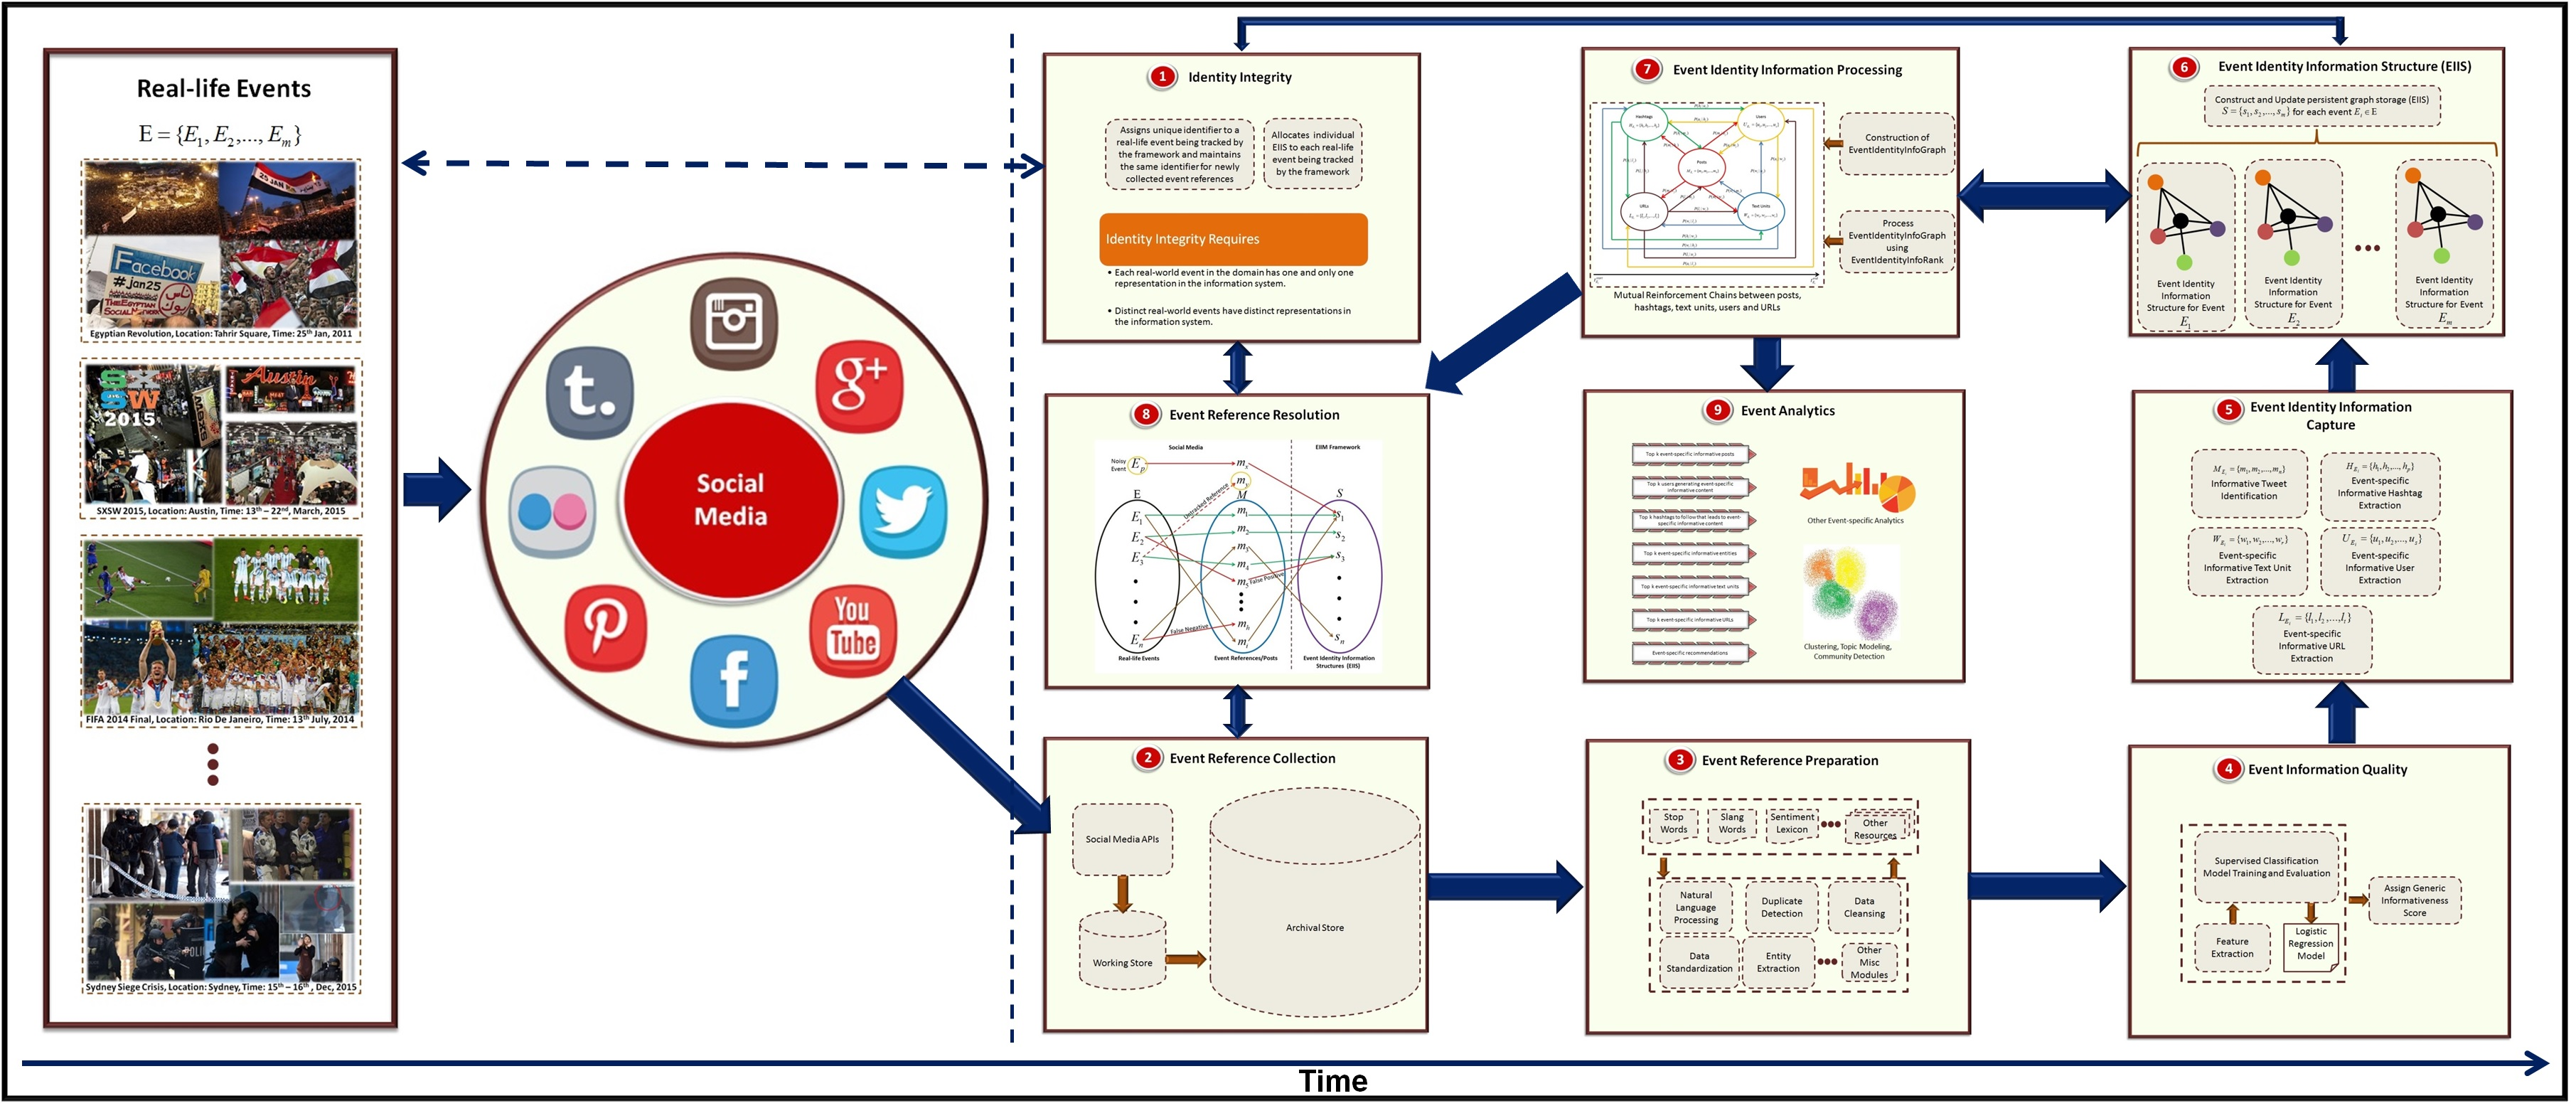
\includegraphics[width=15.5cm,height=7cm]{Figures/EIIM.jpg}
\end{figure}

Some of the main contributions of the work are:

\begin{itemize}
\item Extending the Entity Identity Information Management model  \cite{zhou2011entity} from the closed world domain of Master Data Management (MDM) to the open and unstructured domain of social media.

\item Design and implementation of an \textit{Event Identity Information Management} framework that is capable of tracking and identifying event-specific information from long as well as short user generated textual content in social media. Towards this objective a data processing pipeline named \textit{Event Identity Information Management Life Cycle} is developed (Figure \ref{eiim}), which is capable of :
\begin{itemize}
\item collecting event related real-time content generated in social media
\item pre-processing them using natural language processing techniques
\item identifying high quality informative sources of information
\item extracting event-specific information in order to create \textit{Event Identity Information Structures} (EIIS) for persistently storing and characterizing the salient and high quality event related information 
\item identifying event-specific informative content produced in social media
\end{itemize}


\item Implementation of a supervised classifier in the domain of short and informal social media textual content, for segregating high quality informative messages having higher chances of containing event related information from the low quality non-informative ones. 

\item Analysis of informative and non-informative event related content from 3.8 million short textual social media messages.

\item A novel model that leverages mutually reinforcing relationships between blog posts and named entities mentioned in them, and simultaneously ranks blogs as well as the named entities, allowing identification of event-specific content and further analysis of event-specific information.

\item A novel model based on principle of mutual reinforcement that takes into account the semantics of relationships between short textual \textit{social media messages}, \textit{hashtags}, \textit{text units}, \textit{URLs} and \textit{users}, and represent them in a graph structure - \textit{EvenIdentitytInfoGraph}. A scalable graph processing iterative algorithm -\textit{EventIdentityInfoRank}, is implemented for ranking the nodes of the \textit{EventIdentityInfoGraph}. The algorithm is capable of simultaneously ranking \textit{social media messages}, \textit{hashtags}, \textit{text units}, \textit{URLs} and \textit{users} in terms of event-specific informativeness providing deeper insights into the identity of an event.

\item Evaluate the proposed techniques against popularly used baseline techniques using large scale datasets.

\end{itemize}

Our research publications as well as upcoming publications that represents our contributions related to specific areas covered by the broad area of research as presented in this thesis are given below.

\textbf{\LARGE Related Filed Patent}
\begin{itemize}
\item A System for Collecting, Ranking and Managing Entity Identity Information from Social Media (US 62135258). Inventors: \textbf{Debanjan Mahata} and John R. Talburt, Assignee: The Board Of Trustees Of The University Of Arkansas.
\end{itemize}

\textbf{\LARGE Related Award}
\begin{itemize}
\item \textbf{Debanjan Mahata} and John R. Talburt. \textit{Chatter that Matter : A Framework for Collecting, Extracting, and Managing Event Identity Information from Short Social Media Text}. Student Research and Creative Works Expo, Graduate Competition, University of Arkansas at Little Rock, April, 2015. (Awarded First Place in Engineering and Information Technology).  
\end{itemize}

\textbf{\LARGE Related Publications}
\begin{itemize}
\item \textbf{Debanjan Mahata}, John R. Talburt and Vivek Kumar Singh; \textit{Identifying and Ranking of Event-specific Entity-centric Informative Content from Twitter}. $20^{th}$ International Conference On Applications Of Natural Language To Information Systems (NLDB 2015), Passau, Germany. $17^{th}-19^{th}$ June, 2015.

\item \textbf{Debanjan Mahata} and John R. Talburt; \textit{A Framework for Collecting and Managing Entity Identity Information from Social Media}. $19^{th}$ International Conference on Information Quality, Xi'An, China.

\item \textbf{Debanjan Mahata} and Nitin Agarwal; \textit{Identifying Event-specific Sources from Social Media}. Online Social Media Analysis and Visualization. Lecture Notes in Social Networks, Springer, Kawash, Jalal (Ed). January, 2015.

\item Nitin Agarwal, \textbf{Debanjan Mahata}, and Huan Liu. \textit{Time-and Event-Driven Modeling of Blogger Influence}. Encyclopedia of Social Network Analysis and Mining. Springer New York, 2014. 2154-2165.


\item \textbf{Debanjan Mahata} and Nitin Agarwal. \textit{Learning from the crowd: An Evolutionary Mutual Reinforcement Model for Analyzing Events}. Advances in Social Networks Analysis and Mining (ASONAM), 2013 IEEE/ACM International Conference on. IEEE, 2013.

\item Nitin Agarwal, and \textbf{Debanjan Mahata}. \textit{Grouping the Similar among the Disconnected Bloggers}. Social Media Mining and Social Network Analysis: Emerging Research (2013), 54.

\item \textbf{Debanjan Mahata}, and Nitin Agarwal. \textit{What does everybody know? identifying event-specific sources from social media}. IEEE Fourth International Conference on Computational Aspects of Social Networks (CASoN), 2012.

\item \textbf{Debanjan Mahata} and Nitin Agarwal. \textit{Analyzing Event-specific Socio-Technical Behaviors Through the Lens of Social Media}. The International Sunbelt Social Network Conference (Sunbelt XXXII) organized by the International Network for Social Network Analysis (INSNA), March 12-18, 2012, Redondo Beach, California.

\item Vivek Kumar Singh, \textbf{Debanjan Mahata}, and Rakesh Adhikari. \textit{Mining the blogosphere from a socio-political perspective}. IEEE International Conference on Computer Information Systems and Industrial Management Applications (CISIM), 2010.

\item Vivek Kumar Singh, Rakesh Adhikari, and \textbf{Debanjan Mahata}. \textit{A clustering and opinion mining approach to socio-political analysis of the blogosphere}. IEEE International Conference on Computational Intelligence and Computing Research (ICCIC), 2010.

\end{itemize}

\textbf{\LARGE Related Submitted Publications}

\begin{itemize}
\item \textbf{Debanjan Mahata}, John R. Talburt, Vivek Kumar Singh and Rajesh Piryani; \textit{Chatter that Matter: A Framework for Identifying and Ranking Event-specific Informative Tweets}. $18^{th}$ International Conference on Text, Speech and Dialogue, Plzen, Czech Republic (Notification Due: May 10, 2015)

\item \textbf{Debanjan Mahata}, John R. Talburt and Vivek Kumar Singh; \textit{A Framework for Collecting, Extracting and Managing Event Identity Information from Twitter}. $20^{th}$ International Conference on Information Quality, M.I.T, Boston (Notification Due: April 30, 2015)

\item \textbf{Debanjan Mahata}, John R. Talburt and Vivek Kumar Singh; \textit{From Chirps to Whistles : Discovering Event-specific Informative Content from Twitter}. Proceedings of the $7^{th}$ Annual ACM Web Science Conference. ACM, 2015, Oxford, England (Notification Due: April 30, 2015)

\end{itemize}
  





 

%Twitter alone has 284 million monthly users,  posting 500 million tweets per day produces a variety of content\footnote{\tiny http://about.twitter.com/company}. A significant proportion of it are related to different real-life events (e.g, football matches, conferences, music shows, etc). Majority of this content are personal updates (e.g.  \textit{Thanks for the memories Sochi! I've had the time of my life \#Sochi2014 \#sochiselfie http://t.co/DqkLEaAMpo}), pointless babbles (e.g. \textit{Ted Cruz is a dangerous man. Crazy and gaining support. Megalomaniac leaders are bad, mkay. \#CPAC \#politics \#joke}) and spams (e.g \textit{New post: Sochi Was For Suckers - Laugh Studios/ http://t.co/cWQJCBp3Ow \#lol \#funny \#rofl \#funnypic \#wtf.}). Personal views and conversations might be of interest to a specific group of people. However, they are meaningless and provides no information to the general audience. On the other hand there are tweets that presents newsworthy content, recent updates and real-time coverage of on-going events (e.g. \textit{In \#Sochi, the Dutch are dominating the overall Olympic medal count http://t.co/jMR1WUqEK4 (Reuters) http://t.co/dAfDhEgTGA}). These tweets provide event-specific informative content and are more useful for general audience interested to know about the event. We call them as event-specific informative references. Table \ref{tweetsample} presents some examples of different types of tweets shared during real-life events.
%
%\begin{table}[htbp]
%\centering
%\caption{Examples of different event related tweets.}
%\label{tweetsample}
%     \begin{tabular}{|p{14cm}|} \hline
%     Ted Cruz is a dangerous man. Crazy and gaining support. Megalomaniac leaders are bad, mkay. \#CPAC \#politics \#joke [\textit{\textbf{personal/uninformative}}] \small \textit{\textbf{Event: `CPAC 2014'}}\\ \hline
%     Thanks for the memories Sochi! I've had the time of my life \#Sochi2014 \#sochiselfie http://t.co/DqkLEaAMpo. [\textit{\textbf{personal/uninformative}}] \small \textit{\textbf{Event: `Sochi Games'}} \\ \hline
%     \#SXSW14 \#SXSW \#sxswinteractive \#CPAC2014 \#CPAC \#CPACPickupLines \#CPACPanels Be squared away \@ perky TOP TWEETED of http://t.co/h0igdOVNW0. [\textit{\textbf{spam/uninformative}}] \small \textit{\textbf{Event: `CPAC 2014'}}\\ \hline
%In \#Sochi, the Dutch are dominating the overall Olympic medal count http://t.co/jMR1WUqEK4 (Reuters) http://t.co/dAfDhEgTGA. [\textit{\textbf{event-specific informative}}] \small \textit{\textbf{Event: `Sochi Games'}}\\ \hline
%New post: Sochi Was For Suckers - Laugh Studios/ http://t.co/cWQJCBp3Ow \#lol \#funny \#rofl \#funnypic \#fail \#wtf. [\textit{\textbf{spam/uninformative}}] \small \textit{\textbf{Event: `Sochi Games'}}\\ \hline
%It's \@tedcruz vs. \@SenJohnMcCain in a \#CPAC spat. What did they say? Find out on \#AC360 8p on \@CNN. [\textit{\textbf{event-specific informative}}] \small \textit{\textbf{Event: `CPAC 2014'}} \\ \hline
%     \end{tabular}
%\end{table}


%\section{Background : Entity Identity Information Management in Master Data Management}
%
%
%
%\section{Problem Definition and Research Questions}
%
%\section{General Challenges in Mining Social Media Text}
%
%\subsection{Information Overload}
%A daily average of 58 million tweets is posted in Twitter\footnote{http://www.statisticbrain.com/twitter-statistics/}.On an average 60 million  photos are shared in Instagram daily\footnote{http://instagram.com/press/}. Facebook stores 300 petabytes  of data related to its users from all over the world\footnote{http://expandedramblings.com/index.php/by-the-numbers-17-amazing-facebook-stats/}. These are some compelling statistics that makes social media not only rich in volume of data, but also variety, and the velocity at which data is being generated. Due to the great pace at which data is produced in social media, the search engines and content filtering algorithms often face the problem of information overload \cite{hemp2009death}. They suffer from the dilemma of assessing the accuracy and quality of information content in the sources being produced over their freshness. Thus, collecting different types of references of entities from various social media platforms, assessing their quality, resolving and extracting identity information of the entities poses great challenges in such a situation.
%
%\subsection{Veracity of Sources}
%Judging the accuracy of the information and deciding relevant information content in social media references for the purpose of extracting entity identity attributes constitutes another challenging situation. For trending topics the search engines have started showing real-time feeds from social media websites in their search results. This has attracted spammers who post trending hash-tags or keywords along with their spam content in order to attract people to their websites offering products or services \cite{benevenuto2010detecting}. An alarming 355\% growth of social spam has been reported in 2013\footnote{http://www.likeable.com/blog/2013/11/10-surprising-social-media-statistics/}. Social media has also been instrumental in spreading misinformation and rumors. Spread of misinformation not only results in pandemonium among the users\footnote{http://www.theguardian.com/uk/interactive/2011/dec/07/london-riots-twitter}  but also result in extraction of completely wrong information about entities.
%
%\subsection{Informal Text}
%Unlike sources of news media and edited documents on the web, the textual content of the social media sources are highly colloquial and pose great difficulties in extracting information. One of the most important sources of information about events, prevalent in the domain of social media are the micro-blogging platforms. Micro blogs pose additional challenges due to their brevity, noisiness, idiosyncratic language, unusual structure and ambiguous representation of discourse \cite{bontcheva2013twitie}. Variation in language, less grammatical structure of sentences, unconventional uses of capitalization, frequent use of emoticons, and abbreviations have to be dealt by any system processing social media content. Moreover, various signals of communications embedded in the text in the form of hash-tags (eg.\#sochi), retweets (RT) and user mentions (@) should be understood by the system in order to extract the contextual information hidden in the text. Intentional misspellings sometimes demonstrate examples of intonation in written text \cite{prevost1996information}. For instance, expressions like, `this is so cooool', emphasizes stress on the emotions and conveys more information that should be captured. It has been shown that it is extremely challenging for the state-of-the art information extraction algorithms to perform efficiently and give accurate results for micro-blogs \cite{derczynski2013microblog}. For example, named entity recognition methods typically show 85-90\% accuracy on longer texts, but 30-50\% on tweets \cite{ritter2011named}. Status messages in social networking websites, content in question answering websites, reviews, and discussions in blogs, and forums exhibit similar nature and present similar challenges to information extraction and text mining procedures.
%
%
%
%\subsection{Sampling Bias}
%Most commonly used method for obtaining data samples from social media websites is by using their application programming interfaces (APIs). Given the humungous amounts of data produced in real-time, the APIs cannot provide all the data to every single API requests. The requests are often made through a query interface by passing certain query parameters to the APIs. The amount of data returned against the queries may vary. This depends upon the popularity of the content related to the query. For example, in Twitter studies have estimated that by using Twitter's Streaming API users can expect to receive anywhere from 1\% of the tweets to over 40\% of tweets in near real-time\footnote{https://www.brightplanet.com/2013/06/twitter-firehose-vs-twitter-api-whats-the-difference-and-why-should-you-care/}. The only way to get access to all the tweets is to buy the firehose service, which is seldom done for academic purposes. Other real-time social media publishing services mostly follow the same model. Therefore, this might lead to biasness in the samples collected for studying event related phenomenon and for tracking all the important event related information being produced in real-time.
%
%\subsection{Multiple Data Sources}
%The APIs (Application Programming Interfaces) of the different social media websites returns data in different formats (JSON, XML) using different web standards (REST, HTTPS). Moreover, the information obtained from a social media website is dependent upon the type of content it produces. A video sharing website might return an entirely different set of information from a blogging website. Thus, integrating the data obtained from the various social media platforms for the purpose of extraction and tracking of event related information is also one of the challenges.
%
%\subsection{Lack of Evaluation Datasets}
%There is a lack of ground truth evaluation data for most of the social media text mining tasks. In traditional data mining research, there is often two types of datasets. One of them is known as training dataset and the other is known as test dataset. The models are trained or developed using the training datasets and are evaluated on test datasets. Thus, the test datasets act as the ground truth. The test dataset for various text mining tasks is mostly not available for social media data. It is often the duty of the researchers to create new test datasets in order to solve a specific task in social media. Sometimes this data might not be a benchmark dataset due to various unwanted noise and human error or perception in annotating the data. This might lead to wrong assumptions and false results.
%
%
%\section{Research Methodology}
%
%\section{Research Contributions}
%

The rest of the thesis is organized as follows:

Chapter \ref{events} gives an overview of the different social media websites and challenges in mining information from them. It also looks at the different perspectives of defining an event and gives the definition of events in social media as accepted by the presented work. Finally, it defines the problem of Event Identity Information Management from Social Media whose solution and application is extensively discussed throughout the rest of the thesis.

Chapter \ref{review} reviews the existing literature related to the topic of the thesis and highlights the challenges in applying previously available techniques to the domain of social media. It also discusses the similarities and dissimilarities of our work with the previous ones, and identifies the areas of our novel contributions that makes it different from the available techniques.

Chapter \ref{eiim} presents a detailed discussion of the \textit{Event Identity Information Management Life Cycle}, that is proposed as a solution to the problem that is solved in this thesis. It goes through all the components of the life cycle and gives a detailed explanation of the design choices, implementation and their working.

Chapter \ref{applications} highlights the potential real-life application of the \textit{Event Identity Information Management} framework implemented in this thesis. 

Chapter \ref{Conclusion} draws conclusions of the work presented in this thesis and points to future directions of the work.

% Chapter 2

\chapter{Social Media and Real-life Events} % Main chapter title

\label{events} % For referencing the chapter elsewhere, use \ref{Chapter1} 

\lhead{Chapter 2. \emph{Social Media and Real-life Events}} % This is for the header on each page - perhaps a shortened title

\section{Social Media}
Social media is defined as a group of Internet-based applications that build on the ideological and technological foundations of Web 2.0, and that allow the creation and exchange of user-generated content \cite{kaplan2010users}. These Internet-based applications broadly ranges from blogs, microblogs, media sharing webistes, social bookmarking websites, social news to social networking websites. Brief description of the most popular types of social media websites is given below.

\subsection{Blogs}
A blog can be defined as a website that displays, in a reverse chronological order, the entries by one or more individuals and usually has links to comments on specific postings. Blogs often provide opinions, commentaries, or news on a particular subject, such as food, politics, or local news. Some of them also function as personal online diaries. Most of the time the entries of a blog is archived and is accessible at a later time. For the purpose of constant syndication, RSS or XML feeds for the blogs are made available. An individual entry in a blog is known as a blog post. A typical blog post can combine text, images and links to other blogs, web pages and other media related to its topic. The universe of all the blogs on the Internet is known as blogosphere \cite{agarwal2014time}.

\subsection{Microblogs}
Microblogs are similar to blogs, but a shorter version of it. Most of the microblogging websites pose limitations on the length of an individual post. Twitter, one of the most popular microblogging website has a limitation of 140 characters. This makes the textual posts in these platforms, extremely concise. Users often associate URLs that lead to external sources of information related to the posts. A post may also contain attached image or video. The microblogging services mostly focus on short updates that are pushed out to anyone subscribed to receive the updates. This is made possible by enabling the users to form directed networks of \textit{friends} and \textit{followers}. The \textit{followers} of an user are entitled to get all the updates posted by him. Mostly these updates are public. 

\subsection{Media Sharing}
Media sharing services allow its users to upload and share various multimedia content such as pictures and videos. Most services have additional social features such as profiles, commenting, etc. The most popular are Instagram, Pinterest, YouTube and Flickr. The media elements are often enriched with geographical and topical ``tags'' by the users who create them and the consumers who browse them. These tags acts as very useful meta data and allow automated programs to leverage them for efficient organization and retrieval of the videos and images that otherwise have very less textual content. 

\subsection{Social Bookmarking}
These are the genre of social media services that allow its users to save, organize and manage links to various websites and resources around the internet. Most allow to ``tag" URLs for making them easy to search and share. The most popular are Delicious and StumbleUpon. Some of the services like StumbleUpon also allow their users to form friendship networks. These websites often provide different browsing experiences through interfaces that help the users to search for most recent tags, most popular ones, and so on.

\subsection{Social News}
Social news websites allow people to post various news items or links to articles that are external to the website, and then allows its users to cast their ``vote' on the items. The voting is the core social aspect as the items that get the most votes are displayed most prominently. This makes it an ideal crowdsourced news platform. It is up to the community of users to decide which news items gets seen by more people. Users can also ``tag'' the news stories and comment on them. The most popular are Digg and Reddit.

\subsection{Social Networking}
Social networking websites are the ones that allow its users to connect with each other and form networks. The connections are generally non-directional and reciprocal. Two users who are connected to each other are considered as \textit{friends}. Usually the users in these webistes have a profile that presents the personal information of the user as provided by him. The users have various ways to interact with other users, and also sometimes have the ability to set up groups. These social networks may be based on a certain theme such as interests, location, and profession. Facebook is the most popular personal social network and LinkedIn is the most popular professional network.

Some of the other types of websites that can also be categorized as social media services are, social messaging services, collaboration tools, rating or review sites, personal broadcasting tools, virtual worlds, and group buying. Table \ref{socialmediacat}, lists popular social media websites in different categories. Some of the websites may overlap and fall into multiple categories due to the broad range of services provided by them. For example, Facebook is not only a popular social networking website, but also a widely used social messaging service.

\begin{table}[h]
\centering
\caption{Popular social media websites belonging to different categories.}
\label{socialmediacat}
\begin{tabular}{|c|l|}
\hline
\textbf{Category} & \multicolumn{1}{c|}{\textbf{Popular Social Media Websites}} \\ \hline
\textbf{\textit{Blogs}} & Blogger, Medium, Wordpress, Squarespace \\ \hline
\textbf{\textit{Microblogs}} & Twitter, Tumblr, Posterous \\ \hline
\textbf{\textit{Media Sharing}} & \begin{tabular}[c]{@{}l@{}}Flickr, Instagram, YouTube, Vimeo, Dailymotion, Metacafe,\\ Viddler, Pinterest\end{tabular} \\ \hline
\textbf{\textit{Social Bookmarking}} & Delicious, StumbleUpon, Scoop, Slashdot \\ \hline
\textbf{\textit{Social News}} & Digg, Reddit, Newsvine, Propeller \\ \hline
\textbf{\textit{Social Networking}} & \begin{tabular}[c]{@{}l@{}}Facebook, Google Plus, LinkedIn, Ello, CafeMom,\\ Gather, Fitsugar\end{tabular} \\ \hline
\textbf{\textit{Virtual Worlds}} & Second Life, World of Warcraft, Farmville \\ \hline
\textbf{\textit{Group Buying}} & Groupon, Living Social, Crowdsavings \\ \hline
\textbf{\textit{Personal Broadcasting}} & Blog Talk radio, Ustream, Livestream \\ \hline
\textbf{\textit{Review/Rating}} & Amazon ratings, Angie’s List \\ \hline
\textbf{\textit{Collaboration Tools}} & Wikipedia, WikiTravel, WikiBooks \\ \hline
\textbf{\textit{Social Messaging}} & WhatsApp, Viber \\ \hline
\end{tabular}
\end{table}

According to Pew Research Center Facebook, LinkedIn, Pinterest, Instagram and Twitter are the top five most popular social media websites used by American adult Internet users\footnote{http://www.pewinternet.org/2015/01/09/social-media-update-2014/}. The number of active users world-wide for all the five social media sites is shown in Table \ref{socialmediastat}. The numbers are obtained from the official pages of the respective websites. 

\begin{table}[h]
\centering
\caption{Number of active users for the top five social media websites used by American adults.}
\label{socialmediastat}
\begin{tabular}{|c|c|}
\hline
\textbf{Social Media Website} & \textbf{Number of Active Users} \\ \hline
\textbf{\textit{Facebook}} & 1.31 billion \\ \hline
\textbf{\textit{LinkedIn}} &  347 million \\ \hline
\textbf{Pinterest} & 70 million \\ \hline
\textbf{\textit{Instagram}} & 100 million \\ \hline
\textbf{\textit{Twitter}} & 289 million \\ \hline
\end{tabular}
\end{table}

\section{Characteristics of Social Media Websites\label{char}}
All the above social media websites exhibit certain common characteristics that is also responsible for their wide usage and huge popularity. We revisit some of the characteristics as already suggested by Agarwal et al. \cite{agarwal2010information} in the context of this dissertation.

\begin{enumerate}
\item \textbf{Accessibility:} Social media websites are freely available to whoever has an Internet connection. This makes these websites easily accessible all over the world. One of the latest initiatives by Facebook and Google is to make social media accessible even to the most remote corner of the world through their Internet.org\footnote{http://internet.org/} and ``Loon for All"\footnote{http://www.google.com/loon/} projects, respectively. With the popularity of hand held devices and increase in the Internet bandwidth, social media is accessible to anyone who has a smart phone and can use it. This is unlike the mainstream media or the print media, to which people subscribe and buy in the form of magazines, newspapers, journals, etc. Also, the mainstream media can be easily controlled by the government that may lead to propagation of biased information. For example, during the ``Egyptian Revolution of 2011", the mainstream media was biased, regulated by the government, and did not portray the true picture of the situation in Egypt. On the other hand, it was social media through which people discussed about the actual atrocities of the government and grouped together to incite the entire revolution \cite{hamdy2012framing}.

\item \textbf{Permanence:} Social media websites show dynamic nature and the content can be altered any time.  Users can easily edit the content shared by them. On the other hand the traditional print media and television media is not at all dynamic. Once an article is printed in a magazine/newspaper, or a television show is recorded and broadcasted, it cannot be changed.

\item \textbf{Reach:} As already presented in Table \ref{socialmediastat}, some of the popular social media websites have a reach of billions. Moreover, the ability of an individual user to simultaneously network with many other users makes this reach more effective than any other means of communication. These connections acts as networks of information flow, which helps in spreading any kind of information at a lightning speed \cite{bakshy2012role}. Also it provides equal opportunity to everyone for reaching their intended audience, unlike the traditional mainstream media. This characteristic is now regularly used by politicians for launching election campaigns and reaching out to people in social media \cite{metzgar2009social}. The marketers also leverage social media to a great extent. Event managers also take advantage of it, due to which social media has become an integral part of event management for getting connected with the event audience \cite{socialmediaforevents}. Social media is regularly used during planned events for making announcements, building and tracking audience, building focused communities, developing public relations \cite{eyrich2008pr}, and targeted marketing \cite{mangold2009social}. Due to easy reachability in social media, a focused group of people can also get together very quickly and organize events such as flashmobs and protest movements \cite{sen2012identifying}. 

\item \textbf{Recency:} The time lag at which communication can take place and information can flow is almost zero for the social media websites. Content is produced and communicated in real-time. Once this content is consumed, the users discuss about it instantaneously. Due to the reach and recency of social media it can make people aware of newsworthy events at a faster pace than traditional maintream media \cite{phelan2009using,petrovic2013can}. It might take hours, days, or sometimes months to present news or an event through mainstream media like newspapers, magazines and television. For example, the death of Bin Laden and the entire covert opertation was reported in Twitter even before the US president made an official announcement in the mainstream media \cite{ladendeathnews}. The users in social media were not only aware of the event but were also sharing and discussing it with great zeal.  Another example is of the theater shootings in Colorado \cite{coloradoshooting}. The shooting incident was reported, covered and analyzed in real-time, with traditional news media lagging behind social media by several minutes.

\item \textbf{Usability:} Social media sites are extremely easy to use and are user-friendly. An user does not require special training or skills to create content in a social media website. Whoever, can type or use a device connected to the Internet that enables typing of text can share information in social media. Therefore, the operational cost of any social media application is mostly negligible. This is not the case for mainstream media. In order to report an event one needs to be skilled and specially trained. Also, the printing and telecasting of any event has to go through many other processes and has to be finally approved by the editor. This makes traditional media unusable by common people. The use of social media at the time of Internet blackout during the ``Egyptian Revolution of 2011" is a great example of its usability \cite{egyptianrevinternetblackout}. The Egyptian government had throttled the Internet connection and there was an Internet blackout for hours in order to stop the spreading of messages in social media, which was the major media of communication that led to the protest movements and finally to the revolution. In order to counter attack the government and to allow the Egyptians to use social media for giving latest updates, Google and Twitter launched a service that enabled them to leave a voicemail on a specific number. This voicemail was then posted in Twitter as a text message. Thus, people who didn't have a smart phone or didn't know how to use one could also post messages in social media.

%\item \textbf{Event-specific Information Content:} 

\end{enumerate}

\section{Challenges in Social Media Mining}




\section{Events from Different Perspectives}

\subsection{Topic Detection and Tracking}

\subsection{Automatic Content Extraction}

\subsection{Multimedia Event Detection}

\section{Events in Social Media}

\section{Background: Entity Identity Information Management (EIIM) in Master Data Management}
The idea of Entity Identity Information Management (EIIM) as defined by Zhou et al. \cite{zhou2011entity}, is the collection and management of identity information of real-world entities with the goal of sustaining \textit{entity identity integrity}. \textit{Entity identity integrity} is one of the basic tenets of data quality that applies to the representation of a given domain of real-world entities in an information system \cite{talburt2011entity}. In order to maintain the property of \textit{entity identity integrity} following conditions should be satisfied:

\begin{enumerate}
\item Each real-world entity in the domain has one and only one representation in the information system.

\item Distinct real-world entities have distinct representations in the information system.
\end{enumerate}


Their model of EIIM was motivated by the problem of entity resolution in information systems, particularly in the domain of MDM (Master Data Management). They define entity resolution as the process of determining whether two references to real-world objects in an information system are referring to the same object, or to different object \cite{talburt2011entity}. The EIIM life cycle as proposed by them is an iterative process that combines entity resolution and data structures representing entity identity into specific operational configurations (EIIM configurations, as shown in Figure \ref{originalEIIM}), that when executed in concert, work to maintain the entity identity integrity of master data over time. The EIIM framework is implemented by developing open source software known as OYSTER\footnote{http://sourceforge.net/projects/oysterer/}.

\begin{figure}[htbp]
  \caption{EIIM components and their interactions as proposed in \cite{zhou2011entity}}
\label{originalEIIM}
  \centering
    \includegraphics[width=12cm,height=6cm]{Figures/originalEIIM.jpg}
\end{figure}

Some of the definitions as specified by the current EIIM model are:

\begin{itemize}
\item \textbf{Definition 1.} \textit{An \textbf{entity} (\textbf{$e_{i}$}) is defined as a real-life object that has a distinct identity}.

\item \textbf{Definition 2} \textit{\textbf{Entity Identity Information} is defined as a set of attributes of a given entity that distinctly characterizes it and allows that entity to be distinguished from all the other entities maintained by the framework.}

\item \textbf{Definition 3.} \textit{An \textbf{Entity Identity Information Structure (EIIS)} ((\textbf{$s_{i}$})), is defined as a data structure that can persistently and efficiently store, retrieve, and manipulate entity identity information}.
\end{itemize}

\begin{figure}[htbp]
  \caption{Misjudgments made by EIIM process.}
\label{identityIntegrity2}
  \centering
    \includegraphics[width=10cm,height=10cm]{Figures/eventIdentity.jpg}
\end{figure}

These definitions also hold true for the work presented in this dissertation. The only differences are:
\begin{itemize}
\item We consider a \textbf{real-life event $E_{i}$} as an individual \textbf{entity}.

\item Instead of \textbf{Entity Identity Information}, we define \textbf{Event Identity Information} as a set of attributes that distinctly characterizes it and allows that event to be distinguished from all other events maintained by the framework.

\item Instead of \textbf{Entity Identity Information Structure (EIIS)}, we define 
\end{itemize}



\begin{figure}[htbp]
  \caption{Entity Identity Integrity in EIIM process.}
\label{identityIntegrity1}
  \centering
    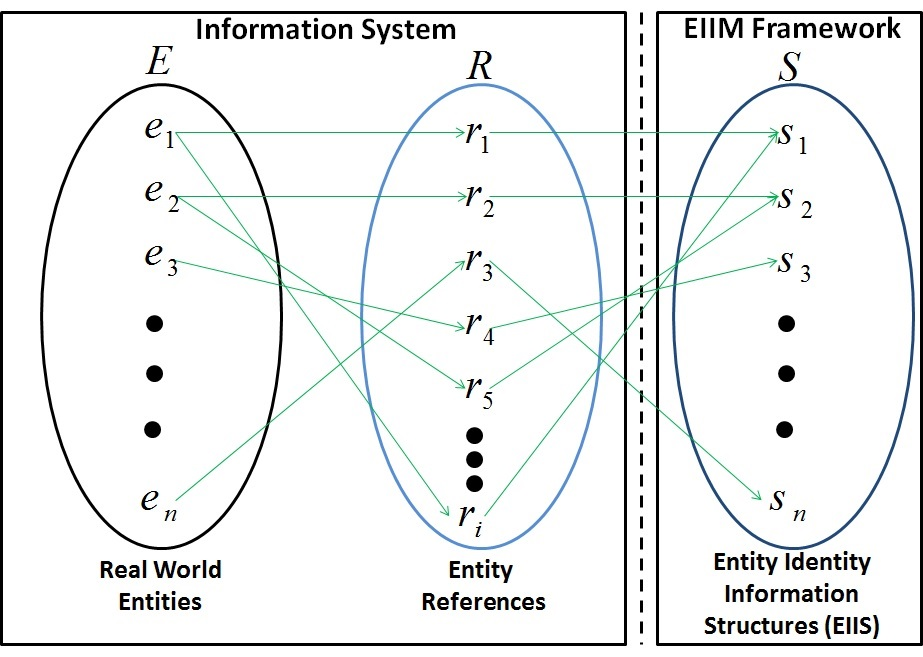
\includegraphics[width=8cm,height=6cm]{Figures/identityIntegrityMDM1.jpg}
\end{figure}



\begin{figure}[htbp]
  \caption{Misjudgments made by EIIM process.}
\label{identityIntegrity2}
  \centering
    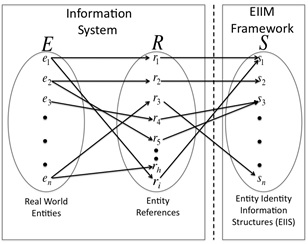
\includegraphics[width=8cm,height=6cm]{Figures/identityIntegrityMDM2.jpg}
\end{figure}


Therefore, ideally in an information system, if $E = \{e_{1},e_{2}, ... ,e_{n}\}$ represents a finite set of entities, $R = \{r_{1},r_{2}, ... ,r_{m}\}$ represents a finite set of references to the entities, and $S = \{s_{1},s_{2}, ... ,s_{n}\}$ represents a finite set of EIIS maintaining identity information of the entities then there should be one-to-one correspondence between the real-life entities ($\in E$) and the EIIS ($\in S$) representing their identity information. Also, the references ($\in R$) of a particular entity ($\in E$) should always map to one and only one EIIS ($\in S$) maintaining its identity information. This is shown in Figure 4. Such a situation ensures that the condition of entity identity integrity is satisfied by the information system. One of the main aims of EIIM is to satisfy the conditions of entity identity integrity along with persistently maintaining the entity identity information.

The current EIIM model deals with a closed environment of an information system where there is fixed number of entities along with fixed number of references to them. In an ideal situation the EIIM process should always satisfy the conditions of entity identity integrity as shown in Figure \ref{identityIntegrity1}, and previously explained. However, in practice, all the references to an entity in the information system might not get mapped to the EIIS maintained for that particular entity due to misjudgments made by the automated processes as shown in Figure \ref{identityIntegrity2}. This might result in false negative and false positive errors. A false negative error arises when the system fails to map a reference of an entity to its corresponding EIIS. This is shown in Figure 5, where the system fails to map the reference $r_{h}$ ($\in R$) of entity $e_{n}$ ($\in E$) to an EIIS ($\in S$). A false positive error arises when the system maps two references of different entities to a single EIIS. This is shown in Figure 5, where the system wrongly maps reference $r_{5}$ ($\in R$) of entity $e_{2}$ ($\in E$), to the EIIS $s_{3}$ ($\in S$) being maintained for entity $e_{3}$ ($\in E$). Such a situation creates dissonance between the actual identity of the real-world entities being stored in the information system and their identities interpreted by the automated processes, resulting in low entity identity integrity of the system. Asserted resolutions are introduced in order to deal with such problems (shown in Figure 3.).

The EIIM processes and life cycle is a step ahead of the basic record linking process that identifies references to same entities for a given dataset. The goal of EIIM is to consistently label references to the same entity with the same identifier across different datasets processed at different times. Through the management of persistent entity identity structures, EIIM provides an added functionality for an entity resolution system to create and assign persistent entity identifiers that do not change from process to process. The current EIIM can also be thought of as forming a nexus between ER and MDM by adding an explicit longitudinal dimension to the management of identity information. The EIIM model proposed in the presented research expands the current model into the unstructured domain of social media, bringing in new challenges and devising new techniques for solving them. The next section gives a detailed discussion and definition of the problem of extending the EIIM model to social media.

\section{Problem of Event Identity Information Management in Social Media\label{problem}}



$\Xi = \{E_{1},E_{2}, ... ,E_{n}\}$

$R = \{r_{1},r_{2}, ... ,r_{m}\}$

$S = \{s_{1},s_{2}, ... ,s_{n}\}$

In this section, we give the definition of an event appropriate in the context of our problem, and then present a formal statement of the problem that we want to solve.

Events have been defined from various perspectives and in different contexts. In the context of our work we adopt a definition similar to \cite{becker2011beyond}. \textbf{Event:} An event is defined as a real-world occurrence ($\scriptstyle E_{i}$) with an associated time period $\scriptstyle T_{E_{i}}$ ($\scriptstyle t^{start}_{E_{i}}$-$\scriptstyle t^{end}_{E_{i}}$) and a time ordered stream of tweets $\scriptstyle M_{E_{i}}$, of substantial volume, discussing about the event and posted in time $\scriptstyle T_{E_{i}}$.
The tweets are primarily composed of a set of hashtags ($\scriptstyle H_{E_{i}}$) used for annotating the tweets ($\scriptstyle \in M_{E_{i}}$), a set of text units ($\scriptstyle W_{E_{i}}$) used for sharing textual information in the tweets ($\scriptstyle \in M_{E_{i}}$), a set of URLs ($\scriptstyle L_{E_{i}}$) linking to external sources related to the event and a  set of users ($\scriptstyle U_{E_{i}}$) posting the tweets ($\scriptstyle \in M_{E_{i}}$).
%\item a set of hashtags ($H_{E_{i}}$) used for annotating the tweets ($\in M_{E_{i}}$) related to the event.
%\item a set of users ($U_{E_{i}}$) posting tweets ($\in M_{E_{i}}$) about the event.
%\item a set of urls ($L_{E_{i}}$) linking to external sources related to the event, shared by the users ($\in U_{E_{i}}$) in the tweets ($\in M_{E_{i}}$) posted by them.
%\item a set of text units ($W_{E_{i}}$) used for sharing textual information in the tweets ($\in M_{E_{i}}$) about the event.


% Chapter 3

\chapter{Literature Review} % Main chapter title

\label{review} % For referencing the chapter elsewhere, use \ref{Chapter1} 

\lhead{Chapter 3. \emph{Literature Review}} % This is for the header on each page - perhaps a shortened title
\doublespacing
\setlength{\parindent}{1cm}
\section{Identifying High Quality Informative Content in Social Media}
Identifying high quality content from the social media feeds that are related to events, is one of the main objectives of our research. As already discussed in Chapter \ref{events}, presence of spams, phishing, farm links, promotion of irrelevant content and development of nepotistic relationships are some of the major concerns of information quality in social media. Several effective solutions has been proposed in combating them by \cite{benevenuto2010detecting,chhabra2011phi,grier2010spam,yardi2009detecting}. Among the different facets of information quality, credibility and trustworthiness of the references are also important.  Due to the popularity and its ability to broadcast information at a tremendous pace, social media is also sometimes used by malicious users to spread misinformation and rumors \cite{tonkin2012twitter}. In such cases, it becomes necessary to assess the credibility and trustworthiness of the information posted. It was showed by Castillo et al. \cite{castillo2011information} that selection of different types of features and automated classification based on supervised training can be used for detecting credible information about newsworthy topics in Twitter. In one of their works \cite{agichtein2008finding} they also proposed a general classification framework for identifying high quality social media content. They took into account the rich meta data like links between items and explicit quality ratings available in Yahoo! Answers website to train a supervised classification model. Credibility of events in Twitter was studied by Gupta et al. \cite{gupta2012evaluating}. They used PageRank for propagating credibility scores on a heterogeneous network of events, tweets and users. They further constructed a graph between similar events and propagated the scores of the events from the previous network to estimate the credibility of other events. Ranking of tweets based on their credibility during trending events was proposed by Gupta and Kumaraguru \cite{gupta2012credibility}. They showed automated extraction of credible information from Twitter, by adopting supervised learning combined with relevance feedback approach using different features mined from tweets and the users posting them. Truthy\footnote{http://truthy.indiana.edu/}, was developed by Ratkiewicz et al. to study information diffusion on Twitter and compute a trustworthiness score for a public stream of micro-blogging updates related to an event to detect political smears, astroturfing, misinformation, and other forms of social pollution \cite{ratkiewicz2011truthy}.


Several mechanisms for ranking social media content in terms of their informativeness have been proposed. Ranking of microblogs like tweets are of particular interest to us as we consider tweets as a representative of short textual content produced in social media. There are many web hosted applications that supplements the default search provided by Twitter in order to effectively retrieve relevant and high quality tweets from different perspectives\footnote{\tiny http://mashable.com/2009/04/22/twitter-search-services}. On going through these services we found that the most commonly used criteria for ranking tweets are recency, popularity based on retweets and favorite counts, authority of the users posting the tweets and content relevance. Twitter itself uses the popularity of the tweets and features mined from the profile of the users in order to provide personalized search results ordered by recency\footnote{\tiny https://blog.twitter.com/2011/engineering-behind-twitter\%E2\%80\%99s-new-search-experience}. A study of different state-of-the-art features and approaches commonly used for ranking tweets has been documented by \cite{Damak2013, nagmoti2010ranking}. Seen\footnote{\tiny http://seen.co} is a new state-of-the-art platform that uses a proprietary algorithm named \textit{SeenRank} for ranking event related tweet content for presenting event highlights and summaries. In this work, we consider \textit{SeenRank} as one of our baselines. As the number of retweets of a tweet is widely used for ranking, we also use it as one of our baselines. In the context of our work we name the ranking scheme as \textit{RTRank}

Apart from the existing real-world search applications, several adaptations of \textit{PageRank} \cite{page1999pagerank} has been proposed by the scientific community for ranking tweets and users in Twitter \cite{weng2010twitterrank,tunkelang2009twitter, hallberg2012adaptation}. TweetRank \cite{hallberg2012adaptation} is one such adaptation that ranks tweets by taking into account the direct relationships between tweets in the form of retweets and replies, as well as indirect follower-friend relationships, and usage of similar hashtags. Various learning to rank approaches have been used for ordering tweets retrieved for a given query in terms of their relevance and quality \cite{Duan2010,mccreadie2013relevance,vosecky2012searching}. None of these ranking techniques have been devised for event-specific content. An attempt to solve a similar problem presented in this paper was made by \cite{becker2011selecting}. They represented tweets of an event in a cluster and calculated the similarity of individual tweets with the centroid of the cluster. Then they ranked the tweets based on the decreasing value of their similarity. We use this approach as one of our baselines.

Recently researchers have shown interest in investigating microblog summarization. Experiments have been conducted using both feature-based and graph-based approaches. However, in the context of our work only graph-based approaches are relevant. A comparison of different Twitter summarization algorithms was performed by \cite{inouye2011comparing}. Summarization of tweets for sporting events was performed by \cite{nichols2012summarizing} using the phrase graph algorithm \cite{sharifi2010experiments}. The popularly used graph-based summarization algorithms are \textit{LexRank} \cite{erkan2004lexrank} and \textit{TextRank} \cite{mihalcea2004textrank}. Both the algorithms make use of the PageRank scheme of ranking homogeneous nodes in a graph constructed from the text that needs to be summarized and identify the salient text units for producing the summary. Our algorithm uses a similar technique for heterogeneous nodes. Our proposed framework also defines the semantics of the relationships between the nodes differently in the context of tweets. We use both \textit{LexRank} and \textit{TextRank} as evaluation baselines.

%Although, we use some of the features used in the works related to ranking tweets and identifying credible content, our approach is entirely different from them. Moreover, we consider only those features that are intrinsic to tweet content. The presented model in this paper is an extension of \textit{Mutually Reinforcing Chain} framework \cite{wei2008}, to the Twitter environment, making our work more related to the graph-based summarization approaches. 

We propose implicit mutually reinforcing relationships between tweets, hashtags, text units, users and URLs forming a heterogeneous graph structure (\textit{TwitterEventInfoGraph}), which is novel and makes our work different from any prior work (refer Chapter \ref{eiim}). Scores are assigned to the association between the nodes representing the semantics of their relationships. We implement an iterative algorithm (\textit{TwitterEventInfoRank}) for ranking the nodes of the graph and propagating the event-specific scores of the nodes to its neighboring nodes based on the measure of their association. To our knowledge, this is the first work that identifies novel relationships between different units of content in Twitter and implements a graph-based algorithm for ranking them simultaneously in the context of an event.

\section{Entity Resolution\label{entityResolutionRelatedWork}}

Entity resolution has been known for more than five decades as the record linkage or the record matching problem in the statistics community \cite{fellegi1969theory,newcombe1959automatic,herzog2007data}. In the database community, the problem is defined as merge-purge \cite{hernandez1998real}, data de-duplication \cite{sarawagi2002interactive,ananthakrishna2002eliminating}, and instance identification \cite{wang1989inter}. In the Artificial intelligence community, this problem is described as database hardening \cite{cohen2000hardening}, and name matching \cite{bilenko2003adaptive}. The names co-reference resolution, identity uncertainty, and duplicate detection are also commonly used to refer to the same task \cite{elmagarmid2007duplicate}. The term Entity Resolution (ER) first appeared in publications by researchers at the Stanford InfoLab led by Hector Garcia-Molina and is defined as the process of identifying and merging records judged to represent the same real-world entity \cite{garcia2006pair}. In the context of the work presented in this thesis a pre-defined real-life event is considered as an entity. For detailed definition of an event please refer Chapter \ref{events}.

Despite the differences in nomenclature used by these authors, the ER process actually comprises five major sub-tasks or activities \cite{talburt2011entity} which are
\begin{enumerate} 
\item	\textit{Entity reference extraction} – locating entity references in unstructured textual information.
\item	\textit{Entity reference preparation} – profiling, standardizing, cleaning, and enhancing reference information in preparation for resolution.
\item	\textit{Entity reference resolution} – the process or algorithm for determining when references are equivalent, often through direct matching of attributes.
\item	\textit{Entity identity management} - creating and maintaining persistent data structures that represent the identities of external entities, the focus of the proposed research.
\item	\textit{Entity relationship analysis} – exploring relationships among distinct entities such as household relationships or shared communication.
\end{enumerate}

The \textit{Event Identity Information Management} Life Cycle (Chapter \ref{eiim}) as proposed in this thesis reflects and implements all of the above activities. Historically the focus of ER research has been on Activity 3, the methods for carrying out the resolution process itself. The majority of published research literature falls into this area. The first formal model for resolution was the Fellegi-Sunter Model of Record Linkage \cite{fellegi1969theory}, which uses a decision-theoretic approach establishing the validity of principles first used in practice by Newcombe \cite{newcombe1959automatic}.  This was followed by the Stanford Entity Resolution Framework (SERF) developed at the Stanford InfoLab \cite{benjelloun2006generic}.  The SERF Model formalizes the generic ER problem as the interaction of two functions for comparing and merging records as black-boxes and defines the conditions required for these functions to give a unique ER result. It also formulates a family of so called ``Swoosh" algorithms (G-Swoosh, R-Swoosh, and F-Swoosh) for carrying out the ER process. With the rise of big data a distributed algorithm D-Swoosh \cite{benjelloun2007d}, was also proposed that can be implemented in a big data environment. More recently the Talburt-Wang Algebraic Model of ER has been proposed \cite{talburt2007algebraic} that views ER as a problem of partitioning a given set of references. 
 
In addition to research on Activity 3, there has also been extensive research in the area of information extraction (IE) that is directly related to the ER Activity 1, reference extraction. The task of entity extraction is also more relevant to social media, due to the unstructured nature of the content. One of the main emphases in the realm of unstructured textual content for last two decades has been in the task of extracting named entities and categorizing them into types. Competitions like MUC (Message Understanding Conference), CoNLL (Conference on Computational Natural Language Learning) and ACE (Automatic Content Extraction) spearheaded the development of new techniques in this domain. This led to the development of sophisticated tools like Stanford NER \cite{finkel2007named}, OpenNLP \cite{baldridge2005opennlp}, GATE \cite{cunningham2002gate}, LingPipe \cite{baldwin2003lingpipe} and NLTK \cite{bird2006nltk}. Variety of techniques ranging from hand-coded rules, automatic rules, to statistical machine learning techniques like hidden Markov models, maximum entropy and conditional random fields have been proposed. A comprehensive survey of the techniques could be found in \cite{piskorski2013information,sarawagi2008information}. A study of various efforts in extracting information from micro-blogs could be found in \cite{hua2012information} and a survey of named entity recognition and classification could be found in \cite{nadeau2007survey}. Efforts have been made by the industry in building crowd sourced knowledge bases like freebase \cite{bollacker2008freebase} and dbpedia \cite{auer2007dbpedia} for the purpose of entity extraction. A recent effort from the industry for extracting entities from social media and building scalable knowledge bases for doing so has been documented in \cite{deshpande2013building,gattani2013entity}. The rise of online social networks, has also motivated new research into the ER Activity 5, entity relationship analysis \cite{bilgic2006d}. With the rise of big data, the modern trend is to perform entity resolution process in humongous volumes of data and scale it horizontally \cite{kolb2012dedoop,talburt2015entity}. In spite of the recent efforts in the field of entity extraction and resolution from unstructured text, there is no generic framework that solves the problem of persistently collecting and managing entity identity information from social media. The development of Event Identity Information Management from social media is a pioneering effort in the field of entity resolution and would create new avenues of research.

Traditionally, entity identity resolution and management (Activity 4) has been a subject of system administration and management of user identities in large organizations. For the first time \cite{zhou2011entity}, showed the intersection of identity management, master data management and entity resolution could be used for managing identities of real-life entities in information systems, that could further play an important role in data integration and information quality. Entity identity management in social media mainly comprises of resolving and integrating profiles of the same person in social networking websites. The FOAF project has been playing an important role in all such efforts \cite{bouquet2010entity,bortoli2007foaf,raad2010user}. A very nice endeavor has been made by the OKKAM project for integrating and managing the multiple entity identifiers in various knowledge bases across the Internet \cite{bouquet2006okkam}. To our knowledge, we are the first to propose a framework for collecting and extracting identity information of events from social media and use the concepts of entity identity management and entity resolution for persistently managing their identities with respect to time.


\section{Event Identification in News Text}
The event detection task \cite{allan2002topic} in the TDT program (Topic Detection and Tracking), led to significant advancements in the field of event-based organization of broadcast news. Some of the efforts in the TDT program focused on online event detection from continuous and real-time streams of textual news documents in newswires \cite{allan1998line,kumaran2004text}. While others explored the detection of past events from archived news documents \cite{yang1998study}. 

The textual content in news documents are different from the short informal text common in the realm of social media.  Most of these documents contain formal text with well-formed grammatical structures, enabling the researchers to rely on the state-of-the-art natural language processing techniques. Named entity extraction and Parts-of-Speech (POS) tagging are among the widely used techniques. Zhang et al. \cite{zhang2007new} extracted named entities and POS tags from textual news documents, and used them to reweigh tf-idf representations of these documents for the new event detection task. Filatova and Hatzivassiloglou \cite{hatzivassiloglou2003domain} identified named entities corresponding to participants, locations, and times in text documents, and then used the relationships between certain types of entity pairs to detect event content. Hatzivassiloglou et al. \cite{hatzivassiloglou2000investigation} used linguistic features (e.g., noun phrase heads, proper names) and learned a logistic regression model for combining these features into a single similarity value. Makkonen et al. \cite{makkonen2004simple} extracted meaningful semantic features such as names, time references, and locations, and learned a similarity function that combines these metrics into a single clustering solution. 

Extracting events from text has been the focus of numerous studies as part of the NIST initiative for Automatic Content Extraction (ACE) \cite{ahn2006stages,ji2008refining}. The ACE program defines event extraction as a supervised task, given a small set of predefined event categories and entities, with the goal of extracting a unified representation of the event from text
via attributes (e.g., type, subtype, modality, polarity) and event roles (e.g., person, place, buyer, seller). Ahn \cite{ahn2006stages} divided the event extraction task into different subtasks, including identification of event keyword triggers, and determination of event
coreference, and then used machine learning methods to optimize and evaluate the results of each subtask. Ji and Grishman \cite{ji2008refining} proposed techniques for extracting event content from multiple topically similar documents, instead of the traditional approach of extracting events from individual documents in isolation. In contrast with the predefined templates outlined by ACE, Filatova et al. \cite{filatova2006automatic} presented techniques to automatically create templates for event types, referred to as domains, given a set of domain instances (i.e., documents containing information related to events that belong to the domain). 

As already discussed, social media documents are extremely concise, noisy and lacks well-established grammatical structures. Therefore, the techniques used in these works are not always suitable for identification of events from social media.  It has been shown that it is extremely challenging for the state-of-the art information extraction algorithms to perform efficiently and give accurate results for micro-blogs \cite{derczynski2013microblog}. For example, named entity recognition methods typically show 85-90\% accuracy on longer texts, but 30-50\% on tweets \cite{ritter2011named}. Therefore, new approaches had to be taken, leading to new techniques for detecting events in social media, which we discuss next.

%One of the goals of the EIIM framework presented in this thesis, is to identify and track event related content being generated in social media. However, the framework does not require detection of unknown events from real-time streams of social media messages. Instead it is provided with a predefined set of events along with predefined hashtags for the respective events, which are used for relevant data collection.

\section{Event Identification in Social Media}
Identification of events and event related content from social media is still in its infancy and needs to be studied more. Several related papers explored the unknown event identification scenario in social media.
Weng and Lee \cite{weng2011event} proposed wavelet-based signal detection techniques for identifying
real-life events from Twitter. These techniques can detect significant bursts or trends
in a Twitter data stream. Sankaranarayanan et al. \cite{sankaranarayanan2009twitterstand}
identified late breaking news events on Twitter using clustering, along with a text-based
classifier and a set of handpicked news seeders. But they do not take into account the filtering of non-event content, which results in poor performance. Segregating the messages that have high likelihood of containing event related informative content from the ones with chances of having non-informative content, or content that are not at all related to an event are at the core of the work presented in this thesis.  Petrovic et al. \cite{petrovic2010streaming} used locality-sensitive hashing to detect the first tweet associated with an event in a stream of Twitter messages. Rattenbury et al. \cite{rattenbury2007towards} analyzed the temporal usage distribution of tags to identify tags that correspond to events. Chen and Roy \cite{chen2009event} used the time and location associated with Flickr image
tags to discover event-related tags with significant distribution patterns (e.g.bursts) in both of these dimensions. Becker et al. \cite{becker2010learning} defined multi-feature similarity metrics based on the textual and non-textual features associated with the social media documents in order to automatically identify events and their related content.
They use the general text-based classifier suggested in \cite{sankaranarayanan2009twitterstand} and a method for identifying top events suggested by \cite{petrovic2010streaming} as baseline approaches in their evaluations and achieved better precision scores.





% but, unlike our work in Chapter 4, they do not filter the vast
%amount of non-event content that exists on Twitter. This, unfortunately, results in poor
%performance, with very low precision scores compared with the precision achieved by our
%methods. Related to our work in Chapters 4 and 5, 



%As we discussed, such text-based and seeder-driven filtering of
%non-event data can be used to generate the event document stream we use in Chapter 5.

 
%
%%We use the general text-based classifier suggested in \cite{sankaranarayanan2009twitterstand} and a method for identifying top events suggested by Petrovic et
%%al. \cite{petrovic2010streaming} as baseline approaches in our evaluation of the unknown identification methods
%%of Chapter 4. While our work in the unknown event identification scenario focuses on timely, online, analysis, several efforts tried to address this task using retrospective analysis. 


New techniques have been proposed recently for identification of known events in social media.
Many of these techniques rely on a set of manually selected terms to retrieve event-related
documents from a single social media site \cite{sakaki2010earthquake,yardi2010tweeting}.  Sakaki et al. \cite{sakaki2010earthquake} developed
techniques for identifying earthquake events on Twitter by monitoring keyword triggers
(e.g., earthquake or shaking). In their setting, the type of event must be known a
priori, and should be easily represented using simple keyword queries. Benson et al. \cite{benson2011event} identified Twitter messages for concert events using statistical models to automatically tag artist and venue terms in Twitter messages.
Their approach is novel and fully automatic, but it limits the set of identified messages for
concert events to those with explicit artist and venue mentions. Most of these approaches are tailored towards one specific social media site. Becker et al. \cite{becker2012identifying} extracts event features, that are often noisy and missing and use them to develop query formulation strategies for retrieving content associated with a planned event from Twitter \cite{becker2011automatic} as well as different social media websites \cite{becker2012identifying}. 




Our method of tracking events is similar to the idea of identification of known events. We also use predefined hashtags and query words to bootstrap the process of collecting data related to a known set of events. However, we introduce and implement the concept of Event Identity Information Structures that are mapped in a one-to-one mapping with the events that we track. The Event Identity Information Structures persistently stores information that acts as identity of an event as the event evolves with time. This identity information is further processed and ranked in order to identify the top event-specific informative units that is further used for tracking new event related content being generated in different social media channels. Also the emphasis of our research is more on information quality, which is absent in most of the previous research in social media. Instead of just identifying event related content, we identify event-specific informative content. Also, the technique that we develop for identifying event-specific informative content from microblogs (Twitter) leverages hashtags, text units, users, posts and URLs. All these metadata are available in most of the social media websites producing short textual content. Therefore our technique should be applicable to other such platforms. We plan to explore it in the future.










%
%%An entity in general may be defined as an object that has a distinct, independent and self-contained existence, whether hypothetical or real. Thus, an entity could be a person (e.g `Barack Obama'), a place (e.g `Little Rock'), a product (e.g `Iphone6'), an event (eg `Egyptian Revolution') or anything from real-life that has an individual identity. The identity of an entity is a set of attribute values for that entity along with a set of distinct rules that allow that entity to be distinguished from all other entities of the same class in a given context [3].
%
%
%\begin{figure}[htbp]
%  \caption{Identity Integrity component of the EIIM life cycle.}
%  \centering
%    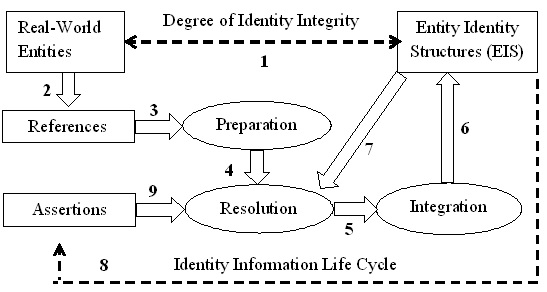
\includegraphics[width=14cm,height=7cm]{Figures/OriginalEIIM.jpg}
%\end{figure} 
%
%In this section we explain the current EIIM process that lays the foundation and acts as a background of the presented research.
%The idea of Entity Identity Information Management (EIIM) as defined by [15] is the collection and management of identity information of real-world entities with the goal of sustaining entity identity integrity. Their model of EIIM was motivated by the problem of entity resolution in information systems, particularly in the domain of MDM (Master Data Management). They define entity resolution as the process of determining whether two references to real-world objects in an information system are referring to the same object, or to different object [16]. The EIIM life cycle as proposed by them is an iterative process that combines entity resolution and data structures representing entity identity into specific operational configurations (EIIM configurations, as shown in Figure 3), that when executed in concert, work to maintain the entity identity integrity of master data over time. The EIIM framework is implemented by developing open source software known as OYSTER .


% Chapter 4

\chapter{Challenges in Mining Event Related Content from Social Media} % Main chapter title

\label{challenges} % For referencing the chapter elsewhere, use \ref{Chapter1} 

\lhead{Chapter 4. \emph{Challenges in Mining Event Related Informative Content from Social Media}} % This is for the header on each page - perhaps a shortened title

The characteristics of social media websites as discussed above in Section \ref{char} makes the domain extremely unstructured and uncontrolled. This gives rise to different challenges in mining information from all types of social media platforms. Some of the major challenges applicable to the context of this dissertation are discussed below. The solutions to these challenges as proposed in this dissertation is also refered while explaining them. Social media posts from the datasets collected for the experiments in Chapter \ref{eiim} (Section \ref{eventreferencecollection}) are presented as examples while discussing the problems.

\section{Information Overload}
A daily average of 58 million tweets is posted in Twitter\footnote{http://www.statisticbrain.com/twitter-statistics/}. On an average 60 million  photos are shared in Instagram daily\footnote{http://instagram.com/press/}. Facebook stores 300 petabytes  of data related to its users from all over the world\footnote{http://expandedramblings.com/index.php/by-the-numbers-17-amazing-facebook-stats/}. These are some compelling statistics that makes social media not only rich in volume of data, but also variety, and the velocity at which data is being generated. Due to the great pace at which data is produced in social media, the search engines and content filtering algorithms often face the problem of information overload \cite{hemp2009death}. They suffer from the dilemma of assessing the accuracy and quality of information content in the sources being produced over their freshness. Thus, collecting different types of references of events from social media, assessing their quality, resolving and extracting identity information of the events poses great challenges in such a situation. 

For example, 284 million monthly users of Twitter posting 500 million tweets per day produces a variety of content\footnote{http://about.twitter.com/company}. A significant proportion of it are related to different real-life events (e.g, football matches, conferences, music shows, etc). Majority of this content are personal updates (e.g.  \textit{Thanks for the memories Sochi! I've had the time of my life \#Sochi2014 \#sochiselfie http://t.co/DqkLEaAMpo}), pointless babbles (e.g. \textit{Ted Cruz is a dangerous man. Crazy and gaining support. Megalomaniac leaders are bad, mkay. \#CPAC \#politics \#joke}) and spams (e.g \textit{New post: Sochi Was For Suckers - Laugh Studios/ http://t.co/cWQJCBp3Ow \#lol \#funny \#rofl \#funnypic \#wtf.}). Personal views and conversations might be of interest to a specific group of people. However, they are meaningless and provides no information to the general audience. On the other hand there are tweets that presents newsworthy content, recent updates and real-time coverage of on-going events (e.g. \textit{In \#Sochi, the Dutch are dominating the overall Olympic medal count http://t.co/jMR1WUqEK4 (Reuters) http://t.co/dAfDhEgTGA}). These tweets provide event-specific informative content and are more useful for general audience interested to know about the event. In this dissertation, we call them as event-specific informative tweets. Table \ref{tweetsample} presents some examples of different types of tweets shared during real-life events. One of the main problems due to information overload is to identify these tweets among millions of tweets being produced during the event.

We develop techniques in this dissertation that helps in overcoming this challenge. In Chapter \ref{eiim} (Section \ref{eventinfoquality}), we develop a generic supervised classifier for Twitter in order to identify event references in real-time from Twitter that has high likelihood of containing high quality information. This results in segregation of informative references from the non-informative ones, and filtering the informative references for further processing. The \textit{EventIdentityInfoRank} algorithm implemented in Chapter \ref{eiim} (Section \ref{eventidentityinformationprocessing}), processes the content in the filtered tweets and results in a ranked list of tweets that has high quality event-specific informative content. 

\begin{table}[htbp]
\centering
\caption{Examples of different event related tweets.}
\label{tweetsample}
     \begin{tabular}{|p{14cm}|} \hline
     Ted Cruz is a dangerous man. Crazy and gaining support. Megalomaniac leaders are bad, mkay. \#CPAC \#politics \#joke [\textit{\textbf{personal/uninformative}}] \small \textit{\textbf{Event: `CPAC 2014'}}\\ \hline
     Thanks for the memories Sochi! I've had the time of my life \#Sochi2014 \#sochiselfie http://t.co/DqkLEaAMpo. [\textit{\textbf{personal/uninformative}}] \small \textit{\textbf{Event: `Sochi Games'}} \\ \hline
     \#SXSW14 \#SXSW \#sxswinteractive \#CPAC2014 \#CPAC \#CPACPickupLines \#CPACPanels Be squared away \@ perky TOP TWEETED of http://t.co/h0igdOVNW0. [\textit{\textbf{spam/uninformative}}] \small \textit{\textbf{Event: `CPAC 2014'}}\\ \hline
In \#Sochi, the Dutch are dominating the overall Olympic medal count http://t.co/jMR1WUqEK4 (Reuters) http://t.co/dAfDhEgTGA. [\textit{\textbf{event-specific informative}}] \small \textit{\textbf{Event: `Sochi Games'}}\\ \hline
New post: Sochi Was For Suckers - Laugh Studios/ http://t.co/cWQJCBp3Ow \#lol \#funny \#rofl \#funnypic \#fail \#wtf. [\textit{\textbf{spam/uninformative}}] \small \textit{\textbf{Event: `Sochi Games'}}\\ \hline
It's \@tedcruz vs. \@SenJohnMcCain in a \#CPAC spat. What did they say? Find out on \#AC360 8p on \@CNN. [\textit{\textbf{event-specific informative}}] \small \textit{\textbf{Event: `CPAC 2014'}} \\ \hline
     \end{tabular}
\end{table}

\section{Veracity of Sources}
Judging the accuracy of the information and detecting relevant, event-specific informative content from social media constitutes another challenging situation due to the malevolent practices of spam users. For trending topics the search engines have started showing real-time feeds from social media websites in their search results. This has attracted spammers who post trending hashtags or keywords along with their spam content in order to attract people to their websites offering products or services \cite{benevenuto2010detecting}. For example, the tweet (\textit{RT @BFDealz: http://t.co/TSJAigrVJI WHEELS SUPER TREASURE HUNT SUPERIZED HARLEY DAVIDSON FAT BOY LONG CARD 2014 \#cpac2014 \#sxsw}) was posted during the parallel occurrence of CPAC 2014 (a political conference) and SXSW 2014, but has nothing to do with the events. Instead it leads to a deal related to Harley Davidson bike promoted using popular event related hashtags \#cpac2014 and \#sxsw. 

An alarming 355\% growth of social spam has been reported in 2013\footnote{http://www.likeable.com/blog/2013/11/10-surprising-social-media-statistics/}. Social media has also been instrumental in spreading misinformation and rumors. Spread of misinformation not only results in pandemonium among the users\footnote{http://www.theguardian.com/uk/interactive/2011/dec/07/london-riots-twitter}  but also result in extraction of completely wrong information about events. The users in the social media websites also develop nepotistic relationships in order to get higher scores in the ranking techniques with malicious intentions \cite{gayo2013nepotistic}. This also helps them to spread spam and other malicious content. Such behavior can also lead to cyber attacks.

Some examples of spam tweets in our collected dataset are shown in Table \ref{tweetsample}. Most of the existing techniques face problems in combating spam.  \textit{EventIdentityInfoGraph} is presented and explained in this dissertation that defines mutually reinforcing chains in Twitter for identifying the most event-specific informative references and filters out the spam tweets after ranking its nodes using \textit{EventIdentityInfoRank}. The algorithm can also identify users who are producing event-specific informative content and URLs (images, videos, news articles) that are extremely relevant to the event. 

\section{Multiple Data Sources with Variety of Content}
The APIs (Application Programming Interfaces) of the different social media websites returns data in different formats (JSON, XML) using different web standards (REST, HTTPS). Moreover, the information obtained from a social media website is dependent upon the type of content it produces. A video sharing website might return an entirely different set of information from a blogging website. Thus, integrating the data obtained from the various social media platforms for the purpose of extraction and tracking of event related information is also one of the challenges.

Although, the type of data and the format of the data returned by the social media services are different, yet most of them have certain common meta-data associated with messages obtained in the responses to the API requests. These are hashtags, text units extracted from the messages/descriptions, the messages itself, the users posting them and the URLs that lead to external sources of related information. Some of the websites where hashtags are not present, the associated tags can be used instead. Table \ref{socialmediametadata} shows the presence of these meta-data in the most popular social media platforms that carry event related information.

\begin{table}[h]
\caption{Presence of different meta-data in popular social media websites.}
\label{socialmediametadata}
\centering
\begin{tabular}{|c|c|c|c|c|c|}
\hline
\textbf{Social Media Website} & \textbf{Hashtags} & \textbf{Users} & \textbf{Text Units} & \textbf{\begin{tabular}[c]{@{}c@{}}Messages/\\ Description\end{tabular}} & \textbf{URLs} \\ \hline
\textit{\textbf{Facebook}} & Yes & Yes & Yes & Yes & Yes \\ \hline
\textit{\textbf{LinkedIn}} & Yes & Yes & Yes & Yes & Yes \\ \hline
\textit{\textbf{Pinterest}} & Yes & Yes & Yes & Yes & Yes \\ \hline
\textit{\textbf{Instagram}} & Yes & Yes & Yes & Yes & Yes \\ \hline
\textit{\textbf{Twitter}} & Yes & Yes & Yes & Yes & Yes \\ \hline
\textit{\textbf{Flickr}} & Yes & Yes & Yes & Yes & Yes \\ \hline
\textit{\textbf{Google Plus}} & Yes & Yes & Yes & Yes & Yes \\ \hline
\textit{\textbf{YouTube}} & Yes & Yes & Yes & Yes & Yes \\ \hline
\end{tabular}
\end{table}  

The developed techniques that are explained in this dissertation rely only upon the above meta-data. This makes the techniques generic and useful for most of the social media channels.
 

\section{Informal Text}
Unlike sources of news media and edited documents on the web, the textual content of the social media references are highly colloquial and pose great difficulties in extracting information. One of the most important sources of information about events, prevalent in the domain of social media are the micro-blogging platforms. Micro blogs pose additional challenges due to their brevity, noisiness, idiosyncratic language, unusual structure and ambiguous representation of discourse \cite{bontcheva2013twitie}. Variation in language, less grammatical structure of sentences, unconventional uses of capitalization, frequent use of emoticons, and abbreviations have to be dealt by any system processing social media content. Moreover, various signals of communications embedded in the text in the form of hash-tags (eg.\#sochi), retweets (RT) and user mentions (@) should be understood by the system in order to extract the contextual information hidden in the text. Intentional misspellings sometimes demonstrate examples of intonation in written text \cite{prevost1996information}. For instance, expressions like, `this is so cooool', emphasizes stress on the emotions and conveys more information that should be captured. It has been shown that it is extremely challenging for the state-of-the-art information extraction algorithms to perform efficiently and give accurate results for micro-blogs \cite{derczynski2013microblog}. For example, named entity recognition methods typically show 85-90\% accuracy on longer texts, but 30-50\% on tweets \cite{ritter2011named}. Status messages in social networking websites, content in question answering websites, reviews, and discussions in blogs, and forums exhibit similar nature and present similar challenges to information extraction and text mining procedures.

In order to solve some of these problems we make use of additional resources in this dissertation that are compiled by us. Some of these resources are list of slang words, list of acronyms and list of stop words commonly used in short social media text (refer Chapter \ref{eiim}). We use these resources in order to aid the natural language processing techniques so that it becomes capable of extracting the required information with higher accuracy. We also experimented with a state-of-the-art entity extraction service AlchemyAPI\footnote{http://alchemyapi.com} and found that the final results obtained using our data processing pipeline are better.



\section{Searching for Information in Long Tail}

\begin{figure}[htbp]
\centering
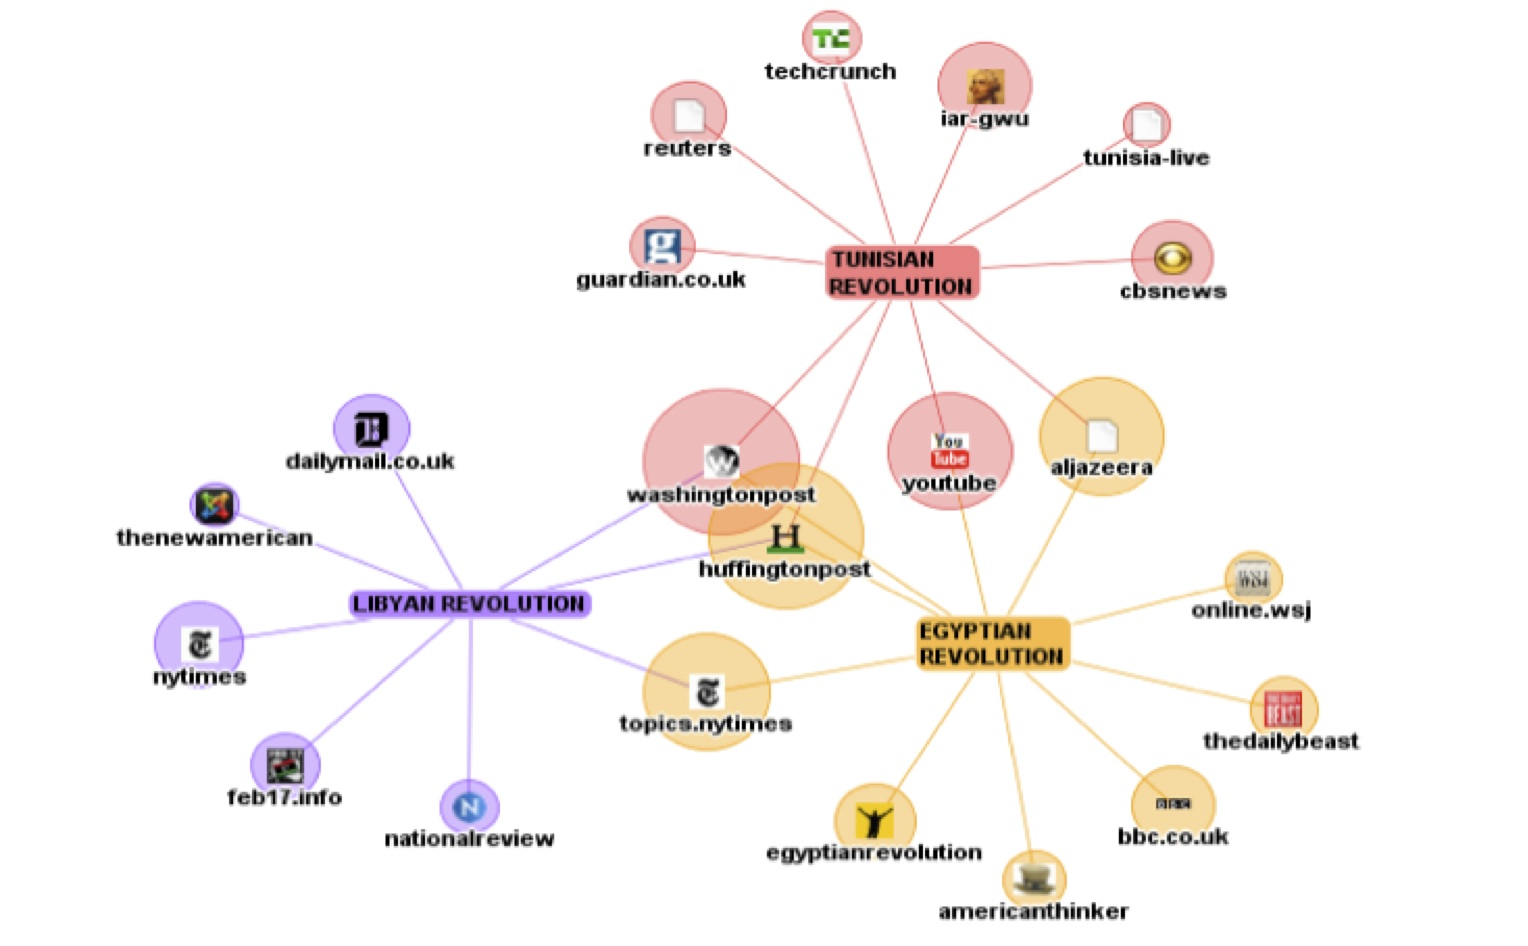
\includegraphics[height=3.5in,width=4.5in]{Figures/Chapter3Figures/touchgraph.jpg} 

\caption{\small Top 10 Google search results for ``Egyptian Revolution'', ``Libyan Revolution'', and ``Tunisian Revolution'', visualized using TouchGraph.}

\label{fg:touchgraph}

\end{figure}

\begin{figure}[htb]
\centering
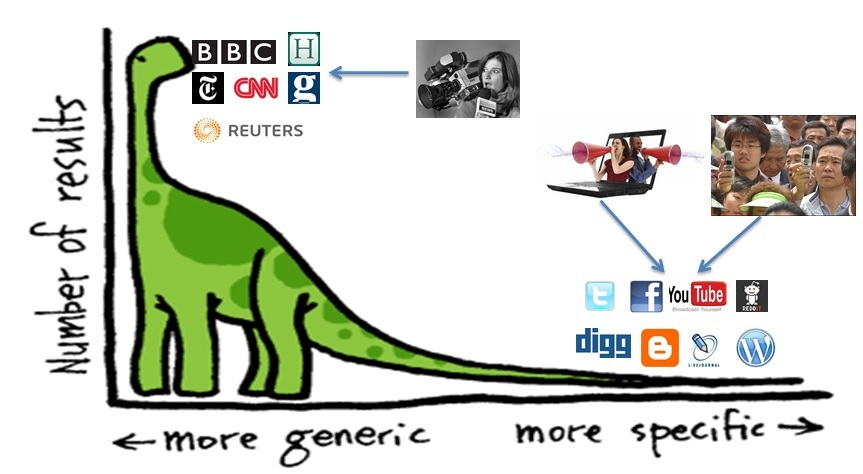
\includegraphics[height=3.3in,width=4.8in]{Figures/Chapter3Figures/LongTailVsShortHead.jpg} 

\caption{\small Short Head Vs Long Tail media sources.}

\label{fg:longvsshort}

\end{figure}


Due to the power law distribution of the Internet \cite{adamic2000power}, and the present search engine technology, the `Short Head' is generally dominated by the mainstream media websites. As illustrated in Figure ~\ref{fg:touchgraph} the top 10 search results for ``Egyptian Revolution", ``Libyan Revolution", and ``Tunisian Revolution" by Google, visualized using Touchgraph\footnote{http://touchgraph.com}, mostly retrieved mainstream media references. Consequently, the social media sites get buried in the Long Tail \cite{LOmariba} as shown in Figure ~\ref{fg:longvsshort}. However, references from the social media channels, act as hubs of specific information about real-life events \cite{harb2011arab}. On the other hand, the mainstream media sources often gloss over the intricate details while covering a real-life event. They are often biased, regulated by the government, and may not portray the true picture of an event \cite{hamdy2012framing}. While, social media references often contain unbiased, uninhibited, and unedited opinions from people. Blogs have been accepted as more credible sources of information over mainstream media references by the weblog users \cite{johnson2004wag}. Thus the references, which are obtained from social media could potentially provide a rather `closer'  or an ``on-ground" view of the events with novel information. The ``on-ground'" information gleaned from the social media affords opportunities to study various online social phenomenon from methodological and theoretical perspectives including, social movements, crowdsourcing, citizen journalism, collective behavior, collective action \cite{agarwal2011finding,agarwal2012online,agarwal2012raising}, and more.

\begin{figure}[htbp]
\centering
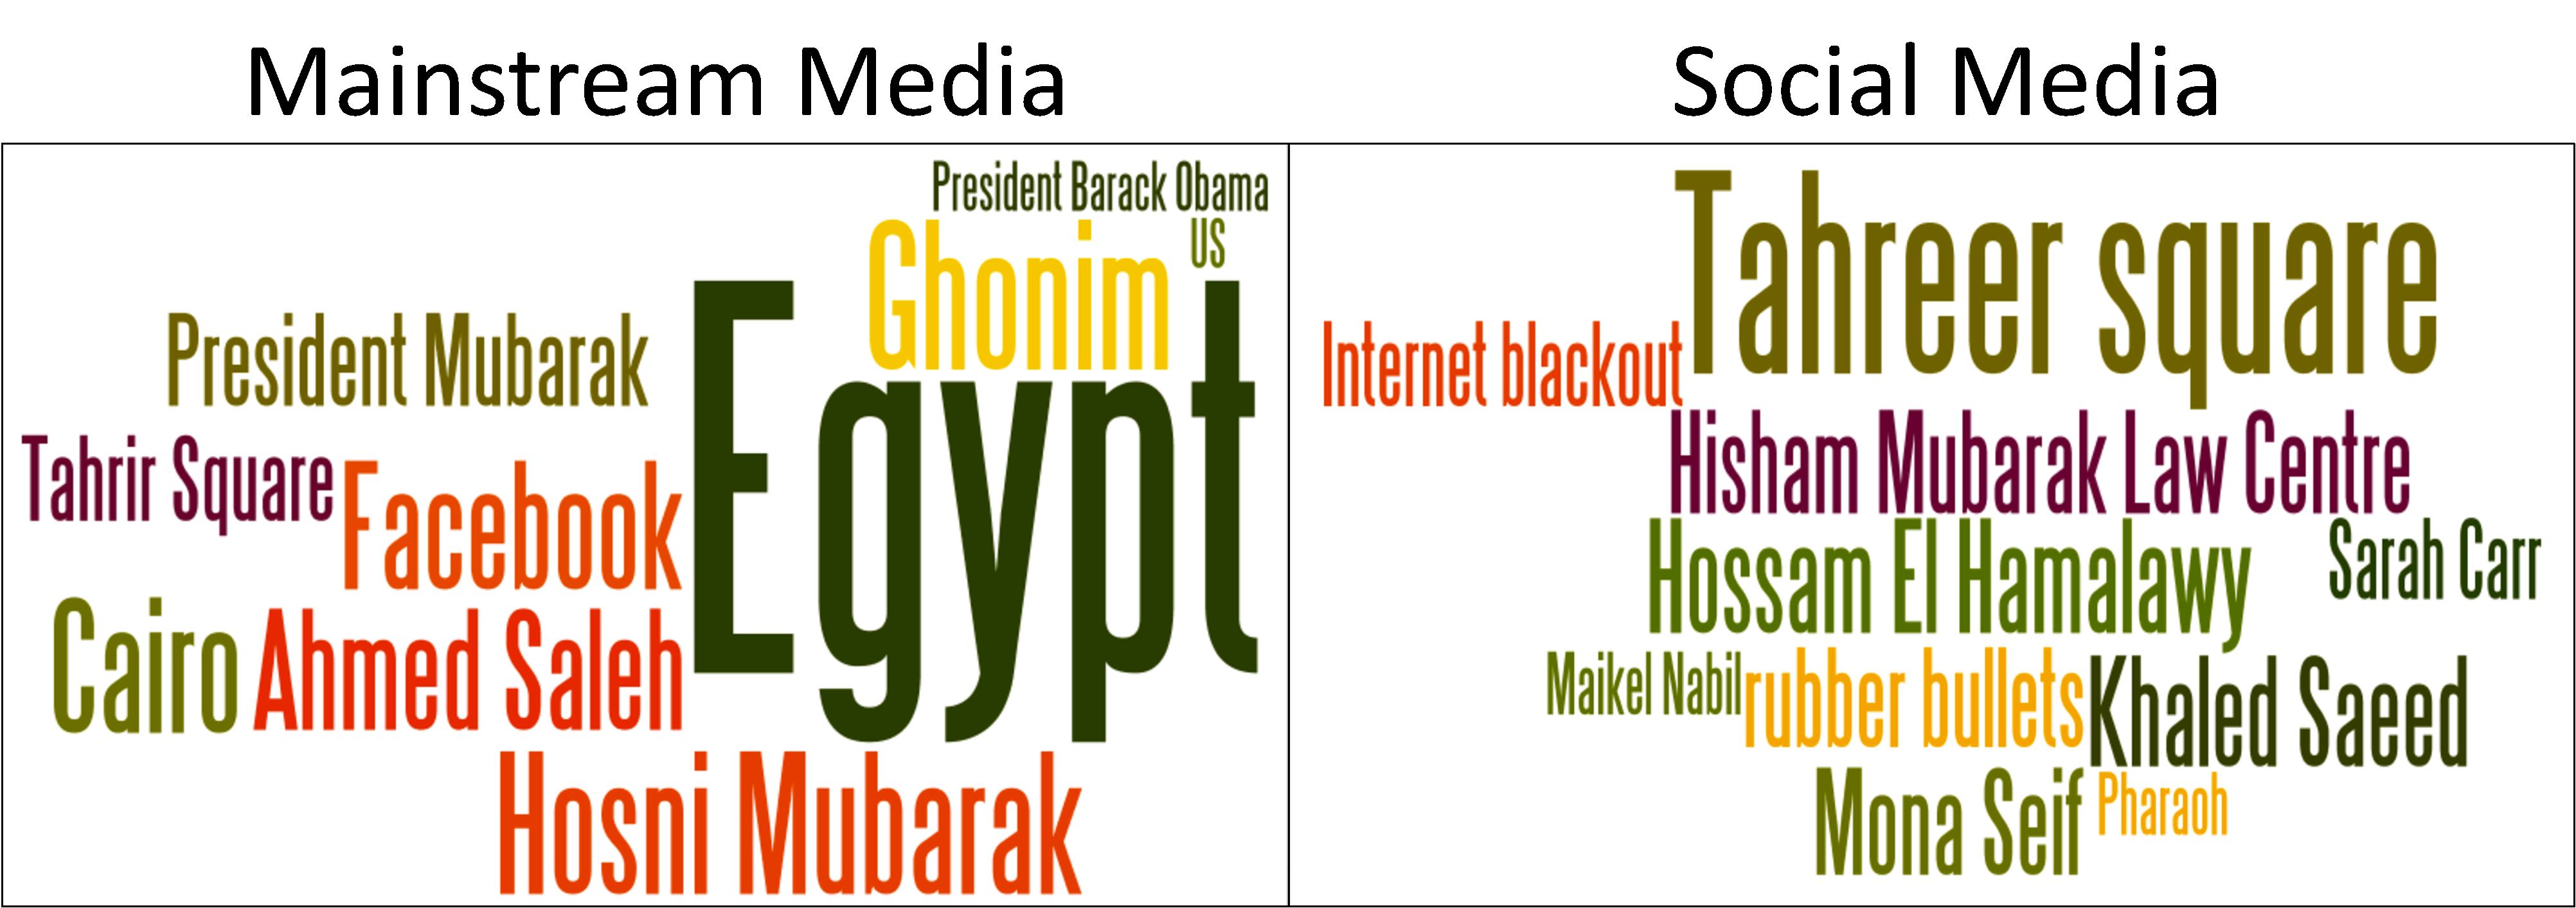
\includegraphics[height=2in,width=4.5in]{Figures/Chapter3Figures/comp.pdf}
\caption{Top 10 entities from mainstream media and blogs.}
\label{fg:comp}
\end{figure}

An initial analysis of the top 10 entities obtained from the top 10 search results related to ``Egyptian Revolution'' from two mainstream media channels (BBC and CNN), and from blogs during the time of the revolution is shown in Figure~\ref{fg:comp}. The top entities from the mainstream media channels are generic and are quiet obvious for the event. In contrast, the top entities from the blogs are very specific to the event. The activists like `Mona Seif', `Sarah Carr', `Maikel Nabil' and `Hosam El Hamalwy' were very closely involved, and were responsible for mobilizing the event. The entities like `Internet Blackout' and `Khaleed Saeed' were central to the event. Moreover, the presence of entities like `Facebook' and `Ghonim' (who was responsible for spreading the event in Facebook) among the top mainstream media entities also indicates the significance of social media in the event.

A person interested to know about an event in detail, may miss out the novel and specific information available in social media by relying on the top results from the popular search engines. It is a challenge for the current ranking schemes to retrieve the event-specific social media content from the long tail. Moreover, in the words of Chris Anderson \cite{anderson2008long}, \begin{itshape} \small ``With an estimated 15 million bloggers out there, the odds that a few will have something important and insightful to say are good and getting better.'' \end{itshape} This also motivated us to look for techniques in this dissertation, that would help in identifying these otherwise buried sources providing highly specific information related to an event.

\section{Sparse Link Structure}
The casual nature of the users posting content in social media channels gives rise to the challenge of sparsity in link structures. Most often the users who posts content, do not provide links to the original source of information. Also, the behavior of linking to other similar content or building reference networks between information posted about the same topic is completely absent among the social media users. This creates an extremely sparse link structure between the user-generated posts. This further creates problems for the traditional and state-of-the-art searching techniques such as PageRank \cite{brin1998anatomy} that performs well in ranking web pages.

In this dissertation, we define novel relationships between content available in the social media channels for solving this issue, and rank them showing better performances than some of the popular baseline techniques.   


\section{Sampling Bias}
Most commonly used method for obtaining data samples from social media websites is by using their application programming interfaces (APIs). Given the humungous amounts of data produced in real-time, the APIs cannot provide all the data to every single API requests. The requests are often made through a query interface by passing certain query parameters to the APIs. The amount of data returned against the queries may vary. This depends upon the popularity of the content related to the query. For example, in Twitter, studies have estimated that by using Twitter's Streaming API users can expect to receive anywhere from 1\% of the tweets to over 40\% of tweets in near real-time\footnote{https://www.brightplanet.com/2013/06/twitter-firehose-vs-twitter-api-whats-the-difference-and-why-should-you-care/}. The only way to get access to all the tweets is to buy the firehose service, which is seldom done for academic purposes. Other real-time social media publishing services mostly follow the same model. Therefore, this might lead to biasness in the samples collected for studying event related phenomenon and for tracking all the important event related information being produced in real-time.


\section{Lack of Evaluation Datasets}
There is a lack of ground truth evaluation data for most of the social media text mining tasks. In traditional data mining research, there is often two types of datasets. One of them is known as training dataset and the other is known as test dataset. The models are trained or developed using the training datasets and are evaluated on test datasets. Thus, the test datasets act as the ground truth. The test dataset for various text mining tasks is mostly not available for social media data. It is often the duty of the researchers to create new test datasets in order to solve a specific task in social media. Sometimes this data might not be a benchmark dataset due to various unwanted noise and human error or perception in annotating the data. This might lead to wrong assumptions and false results.

In this dissertation we find novel ways to validate our results. We rely on both automated as well as manual method of evaluations, as considered appropriate in different scenarios. We use independent annotators for all the annotation tasks, educate them about the tasks and the required information, and also report the percentage of agreement in their performed tasks.
 
% Chapter 5

\chapter{Event Identity Information Management (EIIM) Life Cycle for Social Media} % Main chapter title

\label{eiim} % For referencing the chapter elsewhere, use \ref{Chapter1} 

\lhead{Chapter 5. \emph{Event Identity Information Management (EIIM) Life Cycle for Social Media}} % This is for the header on each page - perhaps a shortened title


%\section{Background : Entity Identity Information Management}

This chapter discusses about the Event Identity Information Management framework in order to solve the problems posed in Chapter \ref{events}, Section \ref{problem}. A high level view of the EIIM components and processes for social media is shown in Figure \ref{eiimcycle}. These components provide a generic framework on which any EIIM system based on social media references could be built. The various components of the framework go through cycles of interactions with each other over time, which is known as EIIM life cycle. At the heart of the framework lies the Event Identity Information Structure (EIIS) and Event Identity Information Processing, which manages the identity information related to a particular event and also helps in resolving high quality, informative references to the event from social media. Next, we give a detailed explanation of each component.

\begin{figure}[htbp]
  \caption{Event Identity Information Management Life Cycle for Textual Content in Social Media.}
	\label{eiimcycle}
  \centering
    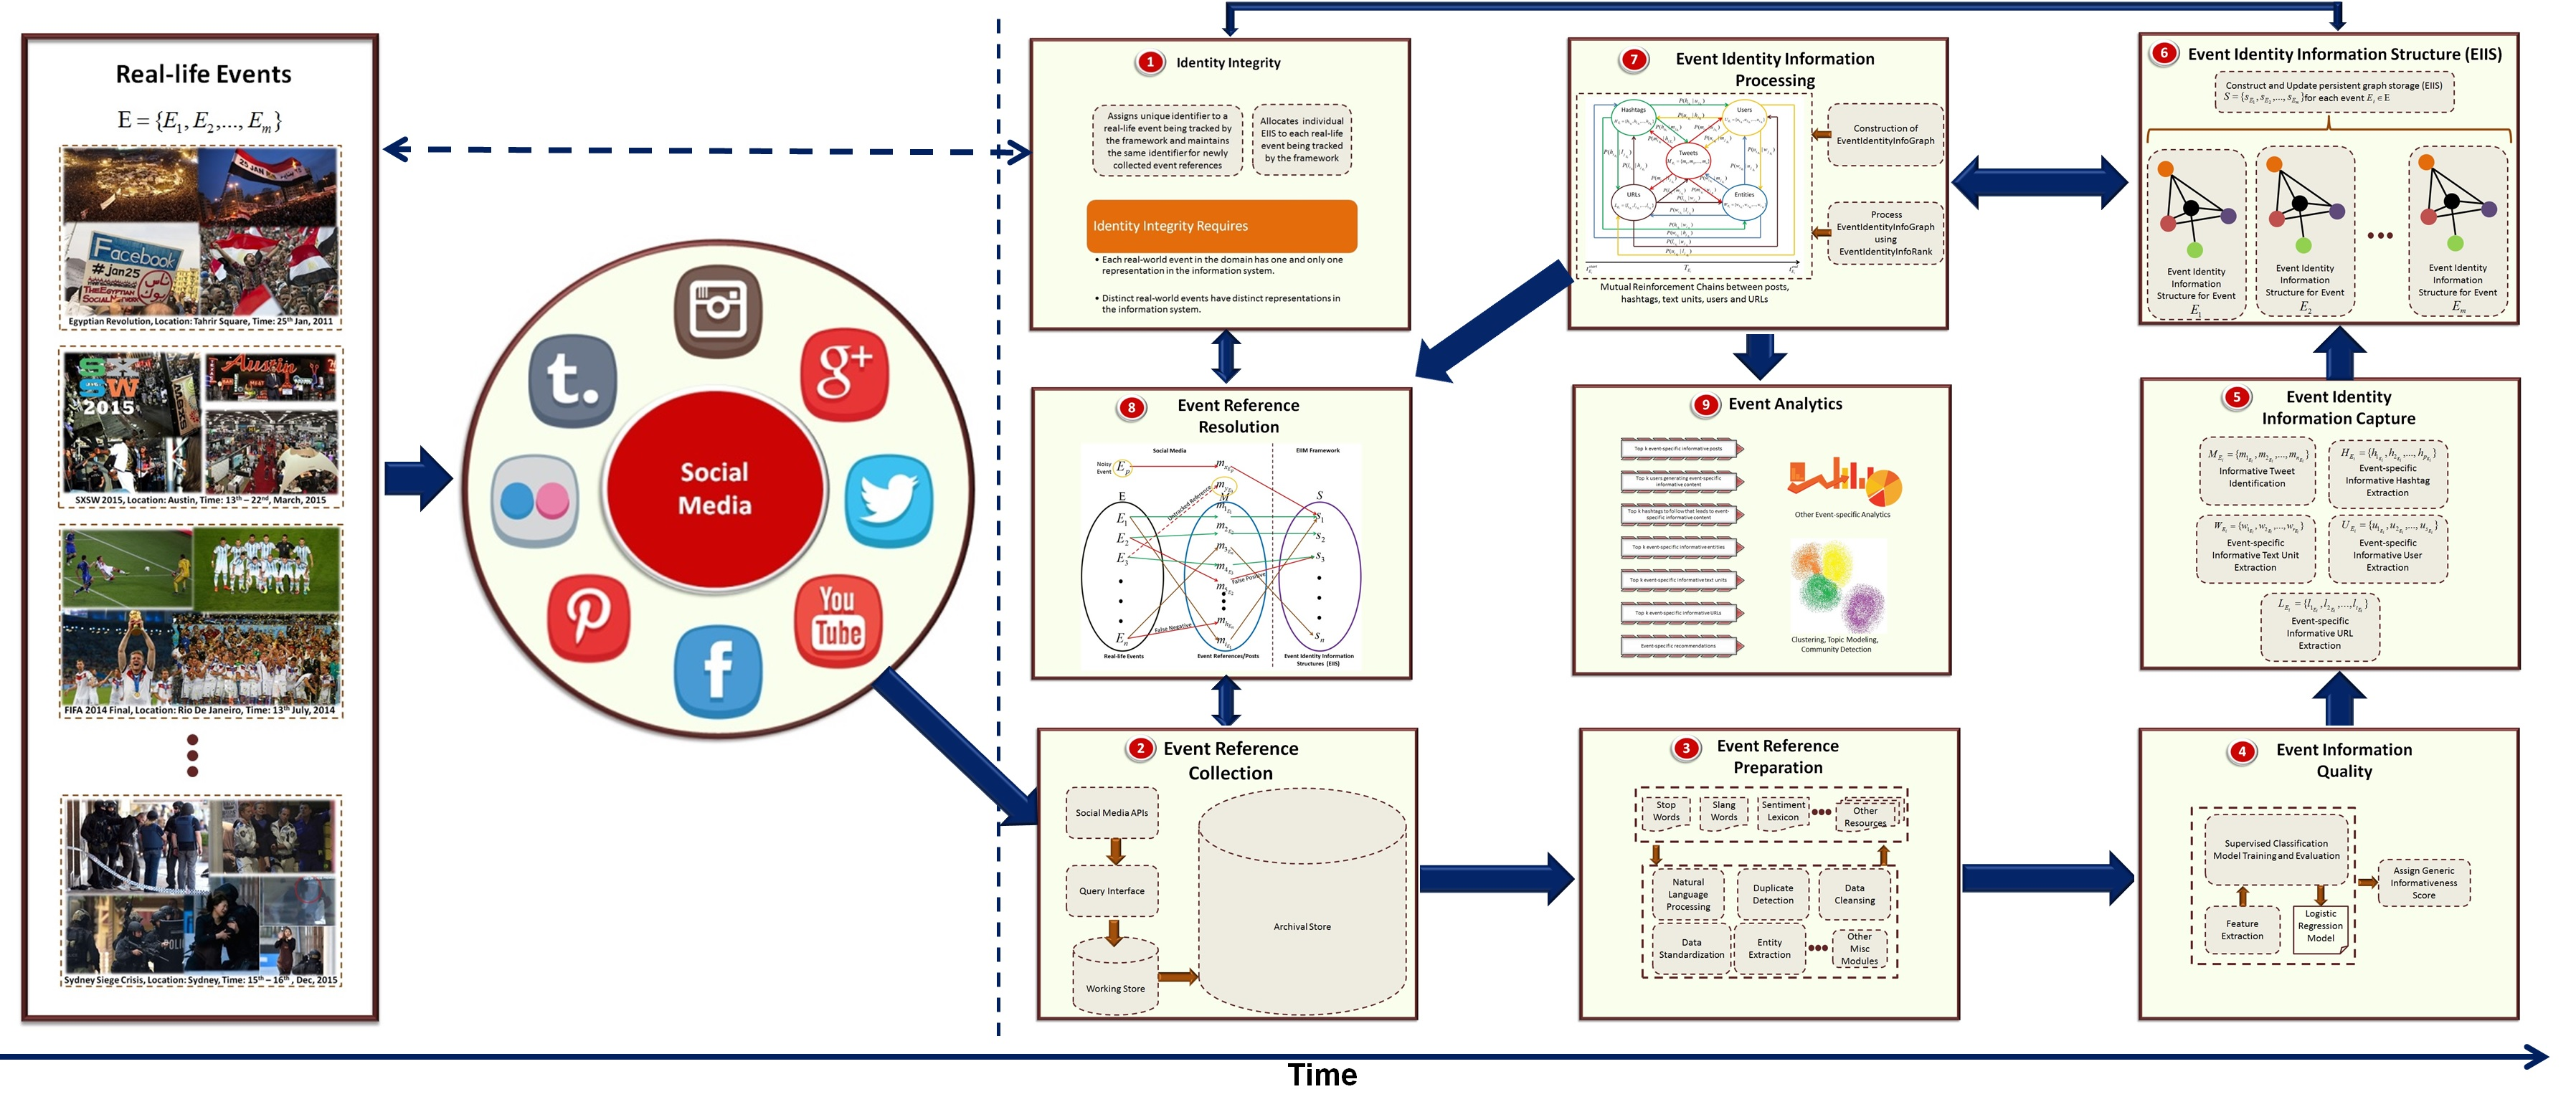
\includegraphics[width=16cm,height=8cm]{Figures/EIIMpic.jpg}
\end{figure}


\begin{figure}[htbp]
  \caption{Identity Integrity component of the EIIM life cycle.}
  \centering
    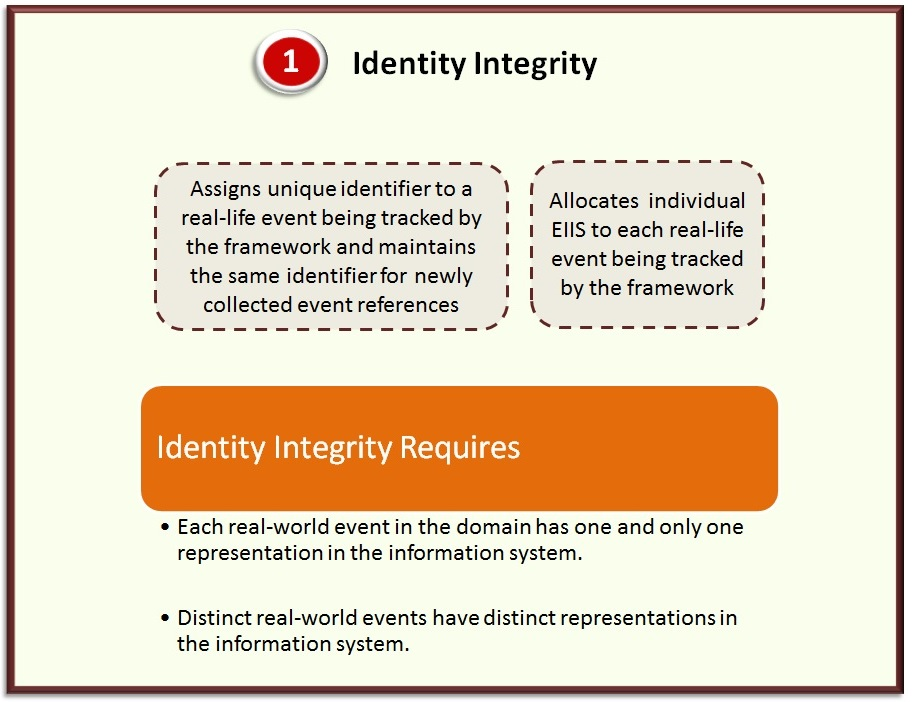
\includegraphics[width=14cm,height=11cm]{Figures/EIIMComponents/IdentityIntegrity.jpg}
\end{figure}

\section{Identity Integrity}
One of the fundamental goals of the proposed framework is to maintain a one-to-one correspondence between real-world events being monitored and the Event Identity Information Structure (EIIS) of the corresponding events for ensuring identity integrity. Therefore, a separate EIIS is maintained corresponding to each event. As new events are introduced to the framework, a unique identifier is assigned to them along with the allocation of individual EIIS structures. The framework is expected to maintain the integrity throughout the EIIM life cycle, by consistently assigning the same identifier to the references of a tracked event. Modules of this component assigns 12 byte unique integers known as ObjectId  to each event, and is also responsible for maintaining the same ObjectId for event ids of collected references and related EIIS. It is also the functionality of this component to assign the right identifier to the references resolved for an event by the Event Reference Resolution component.


\section{Event Reference Collection\label{eventreferencecollection}}

\begin{figure}[htbp]
  \caption{Event Reference Collection component of the EIIM life cycle.}
  \centering
    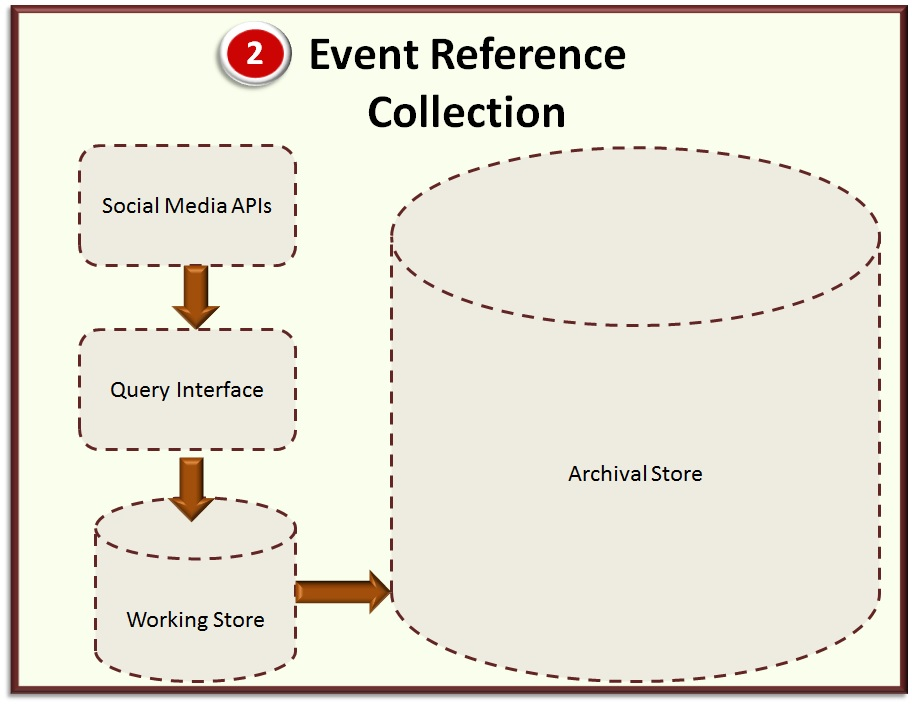
\includegraphics[width=14cm,height=11cm]{Figures/EventReferenceCollection.jpg}
\end{figure}

This component allows the framework to collect event references from different social media websites using its publicly available APIs (Application Programming Interface), and store them in the database after processing them using the next two components of the EIIM life cycle. Due to the semi-structured nature of the collected data, a NOSQL document oriented database management system (MongoDb ) is used for storage. The choice of MongoDb was also driven by its ability to scale horizontally and perform operations on large volumes of data. A query interface is implemented that allows an user of the system to pass query parameters (for example event related hashtags and key words) that bootstraps the data collection and event tracking process. As already shown in Table \ref{socialmediametadata} most of the popular social media channels allow hashtags, the data for the experiments were collected using a popular hashtag for the respective events. 

%For performing the experiments, data was collected from two types of social media websites, 
%\begin{itemize}
%\item \textbf{Blogs} - representing the longer genre of textual references.
%\item \textbf{Microblogs} - representing the shorter genre of textual references.
%\end{itemize}

%The query interface for blogs was implemented separately from the other social media channels as blogs don't provide any API for collecting data. Either one has to scrap data from search engines or monitor the RSS feeds of a pre-specified list of blogs. Details of the data collected is presented next. 

%\noindent \textbf{\textit{Motivation behind source selection:}} For many people blogs have become popular social media sources for satisfying interpersonal communication needs. Blogs act as a platform for masses to share their likes and dislikes, voice their opinions, provide suggestions and report news. Over the years blogging has matured from personal diaries to citizen journalistic sources providing live coverage of events beyond the professional newsrooms. Often mainstream media rely on blogs for reporting first-hand accounts of an event \cite{ekdale2007expression}. Other social media platforms like microblogs, social networks etc., also promote such activities. But, these platforms have very little scope to elaborately discuss about the events due to the limitations in the length of content allowed to be posted. However, these alternative platforms act as good sources for studying and tracking dissemination of information during real-life events. This motivated us to perform our experiments on sources collected from the blogging platforms instead of other social media webs

Due to extreme popularity of Twitter, data from it was collected for representing the microblog genre and short textual social media references. Four million tweets (approx) related to five different events were collected. Details of the collected event references are provided in Table \ref{informationcuedata}. The tweets were collected over the given period of time, by providing a popular hashtag to the Twitter streaming API  as shown in Table \ref{informationcuedata} (for details about Twitter Data Collection please refer Appendix \ref{AppendixA}). Only English language tweets are considered for the experiments as the available natural language toolkits performs well for English, and the annotators used for different tasks are only proficient in English language.

\begin{table}[htbp]
\center
\caption{Details of data collected for analyzing event related tweet content.}
\label{informationcuedata}
\begin{tabular}{|c|c|c|c|}
\hline
\textbf{Event} & \textbf{Query Hashtag}                          & \shortstack{\textbf{No. of} \\ \textbf{Tweets}} & \shortstack{\textbf{Time Period}}                               \\ \hline
\shortstack{Sochi Winter\\ Games 2014 \\ ($http://goo.gl/sG4Rqd$)}& \#sochi2014 & 1958220 & \shortstack{11th Feb,2014\\ to\\ 3rd March, 2014} \\ \hline
\begin{tabular}[c]{@{}c@{}}SXSW 2014  \\ ($http://goo.gl/b6Nd6X$)\end{tabular} & \#sxsw2014                                  & 1880557                                                            & \begin{tabular}[c]{@{}c@{}}8th March, 2014\\ to\\ 16th March, 2014\end{tabular} \\ \hline
\begin{tabular}[c]{@{}c@{}}CPAC 2014 \\ ($http://goo.gl/9o1KUx$)\end{tabular} & \#cpac2014 & 18104                                                              & \begin{tabular}[c]{@{}c@{}}7th March, 2014\\ to\\ 16th March, 2014\end{tabular} \\ \hline
\shortstack{Millions March NYC \\ ($http://goo.gl/I8WR4B$)} & \#millionsmarchnyc  & 56927 & \shortstack{13th Dec, 2014\\ 20:25:43\\ to\\ 14th Dec, 2014\\ 03:30:41} \\ \hline
\begin{tabular}[c]{@{}c@{}}Sydney Siege \\ ($http://goo.gl/qLguvG$)\end{tabular} & \#sydneysiege                                  & 398204                                                            & \begin{tabular}[c]{@{}c@{}}15th Dec, 2014\\ 07:21:16\\ to\\ 15th Dec, 2014\\ 22:46:45\end{tabular} \\ \hline
\end{tabular}
\end{table} 



%\subsection{Blog Reference Collection}
%
%\begin{table}[htbp]
%\centering
%\caption{Details of Data Collected.}
%\label{tab:table1}
%\begin{tabular}{|c|c|c| }
%\hline
%\textbf{Service Used} & \textbf{Event} & \textbf{Number of Blog Posts} \\ [0.5ex]
%\hline
%GlobalVoices & Egyptian Revolution & 234 \\
%&Libyan Revolution & 86 \\
%&Tunisian Revolution & 77\\
%\hline 
%Google Blogger & Egyptian Revolution & 579 \\
%&Libyan Revolution & 600 \\
%&Tunisian Revolution & 484 \\
%\hline
%Icerocket Blog Search & Egyptian Revolution & 5900 \\ 
%&Libyan Revolution & 2198 \\
%&Tunisian Revolution & 1220 \\
%\hline
%\end{tabular}
%\end{table}
%
%%The blog writers, also known as bloggers, loosely form their special interest communities where they debate and discuss issues, spread awareness, gather support, organize and mobilize campaigns - utilizing and in many ways demonstrating the democratic nature of the Internet. 
%
%%
%%\paragraph
%%\noindent \textit{\textbf{Sources:}}
%Blog posts from GlobalVoices, Blogger\footnote{http://blogger.com} and Icerocket Blog Search\footnote{http://icerocket.com} respectively, were collected for the study. The details of the dataset used is given in Table ~\ref{tab:table1}. The dataset includes 11,378 blog posts from various blogging platforms like blogspot.com, wordpress.com, livejournal.com, typepad.com, etc. We also filter out the non-english blogs. The data from GlobalVoices is used for constructing event dictionaries, as explained later in Section \ref{infocapture}. We collect blog posts related to the three events from Blogger using Google Search, and from other blogging platforms using Icerocket blog search. After passing a event related popular word to the query interface, the search engines provided a ranked list of results. The links of the blog posts along with their ranks were obtained by writing a script for screen scraping and stored in the database.
%
%
%%We perform our experiments on the references retrieved by the search engines due to the lack of ground truth and take the references along with the ranks assigned to them by the search engines as our baseline. 
%
%%The collected blog posts are parsed for extracting various information. However, we use the following information for our study: \textit{URL} of the blog and blogpost), \textit{blog text}, \textit{entities}, \textit{language}, and \textit{rank} of the post in the respective search engines used for collecting it. We use AlchemyAPI in order to extract entities. These datasets would be made available on request.
%
%

\section{Event Reference Preparation}

\begin{figure}[htbp]
  \caption{Event Reference Preparation component of the EIIM life cycle.}
  \centering
    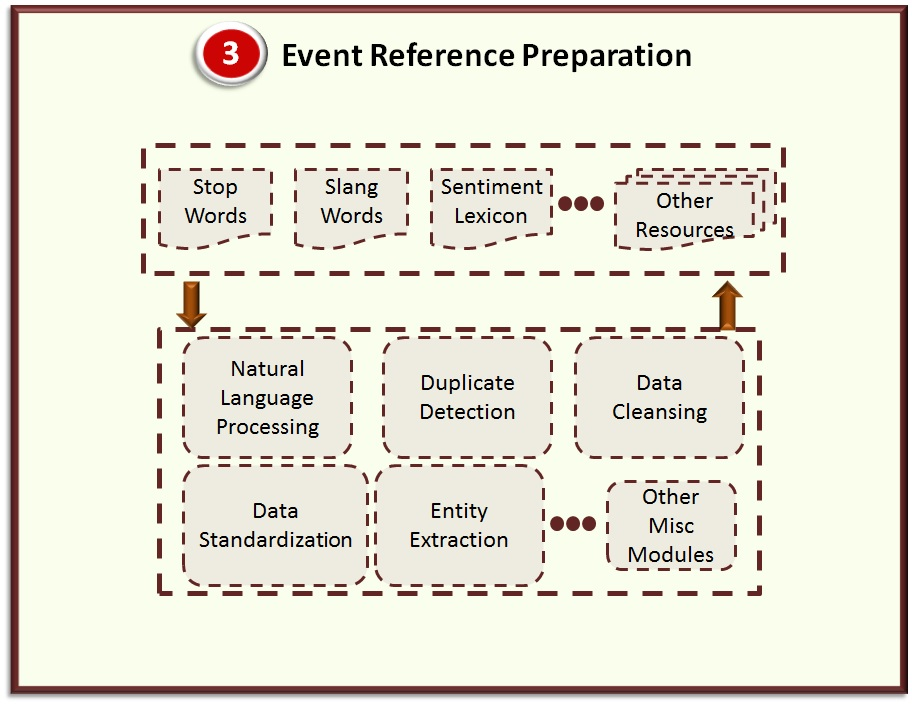
\includegraphics[width=14cm,height=11cm]{Figures/EIIMComponents/EventReferencePreparation.jpg}
\end{figure}

Preprocessing the raw references is an important stage of any data intensive application. This component performs a series of data preparation steps on the collected event references in order to make them suitable for further processing by the other components of the EIIM life cycle. Several resources are compiled in order to tackle the challenges posed by short informal text prevalent in social media. 

%\subsection{Microblog Reference Preparation}

The tweets collected using the previous component goes through the following pre-processing steps:


\subsection{Parts-of-speech tagging} 
The Natural Language Toolkit (http://nltk.org) POS tagger is used for tagging the raw text of the tweets. All the words of a tweet is assigned one of the following parts-of-speech:
\begin{itemize}
\item Noun
\item Adjective
\item Verb
\item Adverb
\item Preposition
\item Interjection
\item Pronoun
\item Article
\end{itemize}

The tagged tweet is also separately stored and maintained. These tags are used later in different components down the pipeline. The Penn Treebank tags\footnote{https://www.ling.upenn.edu/courses/Fall\_2003/ling001/penn\_treebank\_pos.html} are used for tagging and is parsed accordingly for identifying words with a certain parts-of-speech.

\subsection{Special Character Detection}
All the special characters that are not alphanumeric are detected and the total number of special characters in a tweet is stored.


\subsection{Data Cleansing}
The raw text of the tweet is extracted and cleaned. All the user mentions, hashtags, retweet symbols, URLs and special characters are removed and the entire tweet is converted into lowercase. 

\subsection{Duplicate Detection}
The tweets after cleaning are assigned a md5 hash code, which helps in detecting duplicate content. Tweets having the same hash code are considered to be redundant copies of each other, and only a single copy of the tweet is finally stored in the database. This technique also helps in detecting the retweets of a tweet that contain the same content. Also there are certain tweets that are shared with the same content but has different user mentions and with different combination of the words expressing the content. For example, the following tweets talks about the same video shared by mashable and does not present any new information. 

\begin{itemize}
\item RT @mashable: Timelapse video reveals massive size of New York City protests http://t.co/zhqHpkDLk1 \#MillionsMarchNYC http://t.co/WktxssAfDp
\item RT @dianebhartford: ``@mashable: Timelapse video reveals massive size of New York City protests http://t.co/CE0VIyHnLe \#MillionsMarchNYC htt…
\end{itemize}


After the data cleansing step, the duplicate detection scheme identifies both the tweets to be same and only maintain a single copy. This process occurs in real-time. Whenever, a new tweet is obtained from the straming API, the md5 hashcode is calculated after going through the previous data pre-processing steps. A hashtable is maintained in the memory that is constantly searched for the presence of the generated hashcode. If the hashcode is already present then the tweet is dropped and not stored.

\subsection{Stop Word Detection and Elimination}
A list of English stop words is compiled that is publicly shared in the following URL :  
\begin{itemize}
\item https://github.com/dxmahata/EIIMFramework/blob/master/CodeBase/\\EventIdentityInformationManagement/Resources/englishStopwords.txt
\end{itemize}
This list is used for detecting the stop words in English language tweets. The stop words are eliminated and the number of stop words detected is recorded.

\subsection{Slang Word Detection}
Slang words commonly used on the Internet and twitter specific slang publicly shared by FBI\footnote{https://www.documentcloud.org/documents/1199460-responsive-documents.html\#document/p1} is combined together for compiling a list of English slang words. This list is used for detecting and extracting the slang words from the tweets. The number of slang words detected is recorded. This list is also used later to detect the slang hashtags and slang text units.

The compiled list of twitter specific slang words is publicly shared and can be obtained from the following URL : 
\begin{itemize}
\item https://github.com/dxmahata/EIIMFramework/blob/master/CodeBase/\\EventIdentityInformationManagement/Resources/slangWords.txt
\end{itemize}

\subsection{Feeling Word Detection} 
A list of words expressing feelings on the Internet, obtained from wefeelfine.org is used for detecting and extracting the feeling words from a tweet. The number of feeling words detected is recorded and the extracted feeling words are stored. This list is also publicly available and can be obtained from the following URL :
\begin{itemize}
\item https://github.com/dxmahata/EIIMFramework/blob/master/CodeBase/\\EventIdentityInformationManagement/Resources/feelingWords.txt
\end{itemize}

\subsection{Tokenization}
The tweet obtained after performing the data cleansing steps and elimination of stop words are tokenized into unigram and bigram tokens using the tokenizer module available in NLTK. The set of tokens thus obtained are stored separately.

\subsection{Stemming}
The unigram tokens obtained after tokenization are stemmed and a separate list of stemmed tokens are stored. A standard Porter stemmer available with NLTK library is used for the purpose.


\subsection{Tweet Meta-data Extraction}
Several meta-data that are associated with each tweet obtained from the JSON response of the streaming API are extracted.  Some of these meta-data are :
\begin{itemize}
\item Expanded URLs  
\item Hashtags 
\item Retweet Counts 
\item Favorite Counts
\item User Mentions
\item User Follower Counts
\item Verification Information
\item Time Information 
\end{itemize}

\subsection{Named Entity Extraction}
Named entities such as name of persons, animals, places, cars and organizations are extracted from the raw tweets. For this purpose the entity extraction service of AlchemyAPI\footnote{http://alchemyapi.com} is used. 



%It performs deduplication of tweets using md5 hashing scheme. Redundant copies of a tweet are filtered out keeping a single copy in the database. Parts-of-speech tagging is done using the default POS tagger available in the NLTK  module. A standard list of English stop words is used for eliminating the stop words from the tweet text. All the characters of a tweet are converted into lower case and special characters are removed. The tweets are tokenized into unigram tokens. User mentions, retweet symbol and URLs are removed during tokenization and are not considered as tokens.
%
%A list of words expressing feelings in the internet, obtained from wefeelfine.org is used for detecting and extracting the feeling words from a tweet. Slang words commonly used in the internet and twitter specific slang publicly shared by FBI  is combined together for compiling a list of English slang words. The modules use this list for detecting and extracting the slang words from the tweets, hashtags and text units. Retweet counts, favorite counts, verification information, user follower count, time information and expanded form of the URLs shared in the tweets are extracted from the metadata associated with each tweet, as retrieved using the Twitter API. 


\section{Event Information Quality\label{eventinfoquality}}

\begin{figure}[htbp]
  \caption{Event Information Quality component of the EIIM life cycle.}
  \centering
    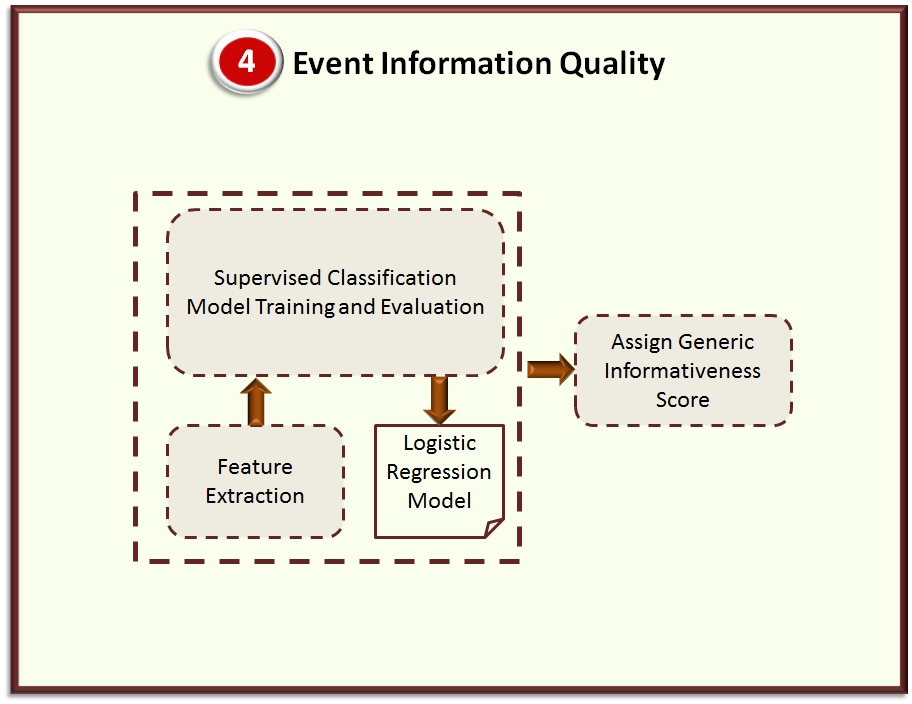
\includegraphics[width=14cm,height=11cm]{Figures/EIIMComponents/EventInformationQuality.jpg}
\end{figure}

This component examines the quality of information present in the tweets collected for the events. It segregates the references having high likelihood of containing good quality event related information from the ones that are less likely to contain or point to good quality information. In order to make a generic module for identifying high quality event related informative references we implemented a logistic regression classifier. Once the classifier is trained, it is used for assigning generic informativeness score to the tweets in real-time as they are collected using the streaming API. The component aids in solving the problem of information overload. Just like an user searching for relevant informative content about an event faces the challenging situation of information overload as discussed in Chapter \ref{challenges}, Section \ref{informationoverload}, it is also a challenge for automated systems to process the huge amount of content coming at high velocity and extract useful information out of it. By filtering out the tweets that are less likely to contain useful and high quality  information it solves the problem of information overload for the other components of the EIIM framework. 

\subsection{Annotated Dataset}
We use a publicly available annotated dataset from the CrisisLex\footnote{http://crisislex.org/data-collections.html} website shared by Olteanu et al. \cite{olteanu2014crisislex}. The collection includes tweets collected during 26 large crisis events in 2012 and 2013, with about 1,000 tweets labeled per crisis for informativeness (i.e. ``informative", or ``not informative"), information type, and source. 28,000 tweets (about 1,000 in each collection) were labeled by crowdsourced workers according to informativeness (informative or not informative), information types (e.g. caution and advice, infrastructure damage), and information sources (e.g. governments, NGOs).

For example, for the Colorado wildfire\footnote{http://en.wikipedia.org/wiki/2012\_Colorado\_wildfires} event, the following tweets were assigned labels of ``related and informative", ``related but not informative", and ``not related", respectively.

\begin{itemize}
\item \textit{Related and Informative} - \#Media Large wildfire in N. Colorado prompts evacuations: Crews are battling a fast-moving wildfire http://t.co/ju1BGTKH \#Politics \#News

\item \textit{Related but not Informative} - RT @LarimerSheriff: \#HighParkFire update \\ http://t.co/hBy5shen

\item \textit{Not Related} - \#Intern \#US \#TATTOO \#Wisconsin \#Ohio \#NC \#PA \#Florida \#Colorado \#Iowa \#Nevada \#Virginia \#NV \#mlb Travel Destinations ; \\ http://t.co/TIHBJKF2
\end{itemize}

Not all the tweets were in English language. We selected English language tweets for training the logistic regression model. There were only 9729 tweets. 

\subsection{Feature Selection and Training}
In order to train the model we assigned a score of 1 to the tweets that were labeled ‘related and informative’, and all the other tweets labeled as ‘related-but not informative’, and ‘not related’ were assigned a score of 0. The choice of features was governed by previous works related to identifying high quality information from Twitter \cite{castillo2011information,gupta2012credibility,vosecky2012searching,huang2011quality}. The list of features selected for the model are: 
\begin{enumerate}
\item \textbf{Has URL} - has a value of 1 if the tweet contains URL or else has a value of 0.
\item \textbf{Number of Words} - total number of unigram tokens extracted from the raw tweet text.
\item \textbf{Number of Stop Words} - total number of English stop words detected in the raw tweet.
\item \textbf{Number of Feeling Words} - total number of feeling words detected in the raw tweet.
\item \textbf{Number of Slang Words} - total number of slang words detected in the raw tweet.
\item \textbf{Number of Hashtags} - total number of hashtags used in the raw tweet.
\item \textbf{Number of User Mentions} - total number of user mentions detected in the raw tweet.
\item \textbf{Tweet Length} - total number of characters used in the raw tweet.
\item \textbf{Unique Characters} - total number of unique characters used in the raw tweet.
\item \textbf{Special Characters} - total number of special characters detected in the tweet.
\item \textbf{Favorite Count} - total number of favorite count of the tweet at the time it was collected.
\item \textbf{Retweet Count} - total number of retweet count of the tweet at the time it was collected.
\item \textbf{Verified} - has a value of 1 if the user posting the tweet is a verified user by Twitter or else has a value of 0.
\item \textbf{Number of Nouns} - total number of nouns detected in the tweet, without considering the hashtags and the user mentions whenever they are tagged as nouns.
\item \textbf{Number of Adjectives} - total number of adjectives detected in the tweet, without considering the hashtags and the user mentions whenever they are tagged as adjectives.
\item \textbf{Number of Verbs} - total number of verbs detected in the tweet, without considering the hashtags and the user mentions whenever they are tagged as verbs.
\item \textbf{Number of Adverbs} - total number of adverbs detected in the tweet, without considering the hashtags and the user mentions whenever they are tagged as adverbs.
\item \textbf{Number of Pronouns} - total number of pronouns detected in the tweet, without considering the hashtags and the user mentions whenever they are tagged as pronouns.
\item \textbf{Number of Interjections} - total number of interjections detected in the tweet, without considering the hashtags and the user mentions whenever they are tagged as interjections.
\item \textbf{Number of Articles} - total number of articles detected in the tweet, without considering the hashtags and the user mentions whenever they are tagged as articles.
\item \textbf{Number of Prepositions} - total number of prepositions detected in the tweet, without considering the hashtags and the user mentions whenever they are tagged as prepositions.
\item \textbf{Formality} - which is defined as follows,
Formality = (\#nouns + \#adjectives + \#prepositions + \#articles - \#pronouns - \#verbs - \#adverbs - \#interjections + 100)/2
and is proposed in \cite{alejandro2011use}. \#nouns, denotes the number of nouns detected in the tweet, and so on.

\end{enumerate}


\begin{table}[htbp]
\centering
\caption{Evaluation measures for logistic regression model.}
\label{logregreseval}
\begin{tabular}{c|c|c|c|}
\cline{2-4}
\multicolumn{1}{l|}{}                          & \textbf{Precision} & \textbf{Recall}       & \textbf{F1-score}     \\ \hline
\multicolumn{1}{|c|}{\textbf{Non-informative} (0)} & 0.70               & 0.49                  & 0.57                  \\ \hline
\multicolumn{1}{|c|}{\textbf{Informative} (1)}     & 0.78               & 0.90                  & 0.84                  \\ \hline
\multicolumn{1}{|c|}{\textbf{Avg/Total}}       & 0.76               & 0.77                  & 0.75                  \\ \hline
\multicolumn{1}{|c}{\textbf{Accuracy}} =  & \multicolumn{1}{l}{} 76.64\%            & \multicolumn{1}{l}{} & \multicolumn{1}{l|}{} \\ \hline
\end{tabular}
\end{table}


\subsection{Model Evaluation}

10-fold cross validation was performed, with `l1' penalty, resulting in a model with an accuracy of 76.64\%. Table \ref{logregreseval} lists the evaluation measures obtained while training the classifier. The ROC AUC Score of the classifier is 0.6934.

\subsection{Assignment of Generic Informativeness Score}
The trained model is used for assigning a score between 0 (least informative) and 1 (most informative) to the tweets in real-time. Both the ‘Event Reference Preparation’ and the ‘Event Information Quality’ components work in collaboration with the ‘Event Reference Collection’ component in order to collect, prepare, assign quality score and store the tweets related to an event, obtained from Twitter streaming API, in real-time.



%\begin{savenotes}
%\begin{table}[ht]
%\centering
%\caption{Tweet features for content informativeness.}
%\label{tweetfeature}
%\begin{tabular}{|l|}
%\hline
%Has Url, No. of words, No. of stopwords, No. of feeling words, No. of slang \\ 
%words, No. of hashtags, No. of user mentions, Tweet  length (No. of characters),\\  No. of unique 
%characters, No. of special characters, Favorite count, Retweet \\ count, Formality, Is tweet verified, No. of nouns, No. of adjectives, No. of \\ verbs, No. of adverbs, No. of pronouns, No. of interjections, No. of articles, \\ No. of prepositions.
% \\ \hline
%\end{tabular}
%\end{table}
%\end{savenotes}



%\subsection{Analysis of Informative and Non-informative Content in Twitter}

\section{Event Identity Information Capture\label{infocapture}}

\begin{figure}[htbp]
  \caption{Event Identity Information Capture component of the EIIM life cycle.}
  \centering
    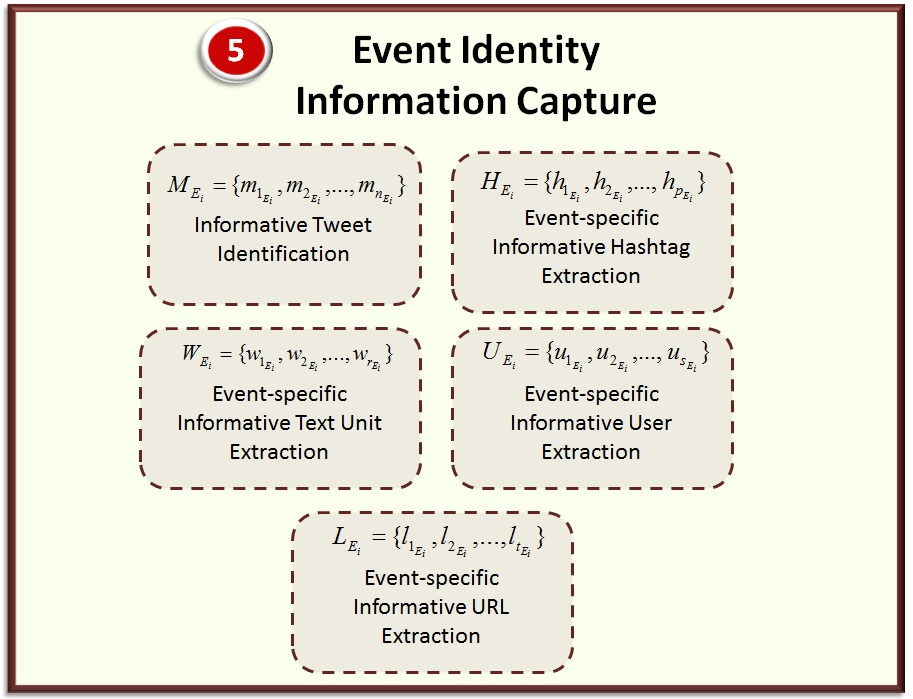
\includegraphics[width=14cm,height=11cm]{Figures/EventIdentityCapture.jpg}
\end{figure}

The main functions of this component are:
\begin{itemize}
\item This component aids in extracting event identity information units (explained later) from the already processed tweets and build the Event Identity Information Structure (EIIS) for an event.
\item It enables the framework to set a threshold between 0.0-1.0 for differentiating between high quality informative tweets from low quality non-informative ones related to an event. The event identity information units are then extracted from the high quality informative tweets.
\end{itemize}
  
In order to understand what might consist of the event identity information units that would represent the EIIS, we conducted a detailed analysis of 3.8 million tweets collected for following three events. 
\begin{itemize}
\item CPAC 2014.
\item SXSW 2014.
\item Sochi Winter Games 2014.
\end{itemize}
The analysis and the conclusions we made from it, is presented next.

\subsection{Content Analysis of Event Related Tweets}
Details of the data collected for the analysis are provided in Table \ref{informationcuedata}. The data collection task was accomplished by `Event Reference Collection' component and was then preprocessed by the `Event Reference Preparation' component.

Twitter allows its users to post short messages with a limitation of 140 characters. Users not only post plain textual content in their messages but also share URLs, linking to other external websites, images and videos. The images and videos are 
labeled as media elements by Twitter. Apart from curating new content, the users also share content produced by others. This activity is known as \textit{retweeting}, and such tweets are preceded by the special characters \textit{RT}.
The messages are normally written by a single person and are read by many. The readers in the context of Twitter are known as \textit{followers}, and the user whom the other users follow is considered as their \textit{friend}. Any user with good intent either share messages 
that might be of interest to his followers, or for joining conversations on topics of his interest. The `@' symbol followed by the username commonly known as \textit{user mentions}, is used for mentioning other users in tweets for initiating conversation with them. 

The concise and informal content of a tweet is often contextualized by the use of a crowdsourced annotation scheme called \textit{hashtags}. Hashtags are a sequence of characters in any language prefixed by the symbol `\#' (for e.g. \#icwsm2015). They are widely used
by the users in order to add context to the tweets, categorizing the content based on a topic, join conversations related to a topic, and to make the tweets easily searchable by other interested users. They also act as strong identifiers of topics \cite{laniado2010making}. When tweeting about real-life
events the users also tend to use hashtags in order to post event-specific content. For example `\#Egypt' and `\#Jan25', were among the most popular hashtags in Twitter used for spreading, organizing and analyzing information related to `Egyptian Revolution of 2011' \cite{barrons2012suleiman}. 

Given the mechanisms of user interactions and content production in Twitter, we started our analysis with the assumption that the content of a tweet is primarily composed of hashtags, words for expressing and conveying information, and URLs that lead to additional information about the content. We plotted the distribution of occurrences of all the hashtags, tokens and shared URLs for each event. Due to the short length of the tweets we only considered unigram tokens. We also plotted the distribution of the number of tweets posted by the users.
We observed a power law distribution for all of them (refer Figures \ref{hashtagdist}, \ref{tokendist}, \ref{urldist} and \ref{userdist}). This gave us an intuition that there are skewed sets of hashtags and tokens that are widely used for posting content related to an event. 
%We call them \textit{event-specific hashtags} and \textit{event-specific text units}. 
There is also a specific set of URLs that become popular in comparison to others and a set of users who are more active than others in posting event related content. 

\begin{figure}[htbp]
  \caption{Distribution of hashtags in event related tweets.}
	\label{hashtagdist}
  \centering
    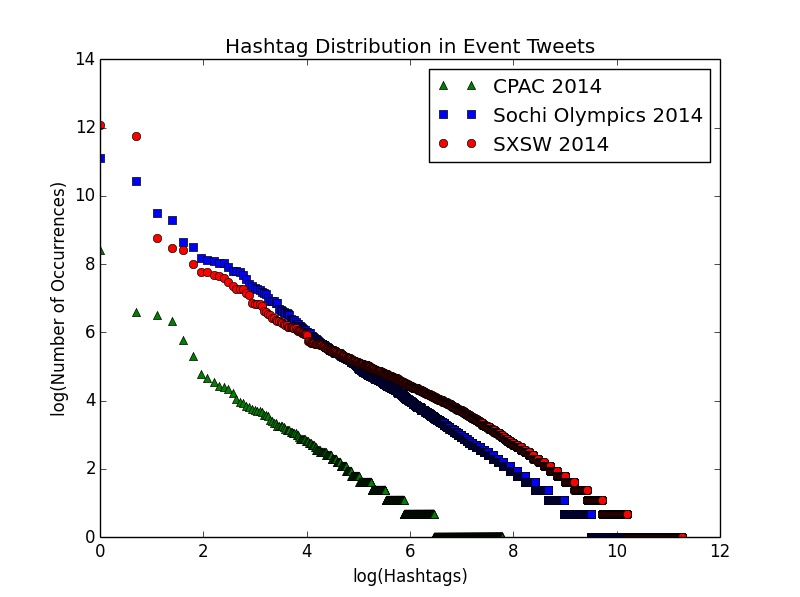
\includegraphics[width=14cm,height=11cm]{Figures/HashTagDistribution.jpeg}
\end{figure}

\begin{figure}[htbp]
  \caption{Distribution of tokens in event related tweets.}
\label{tokendist}
  \centering
    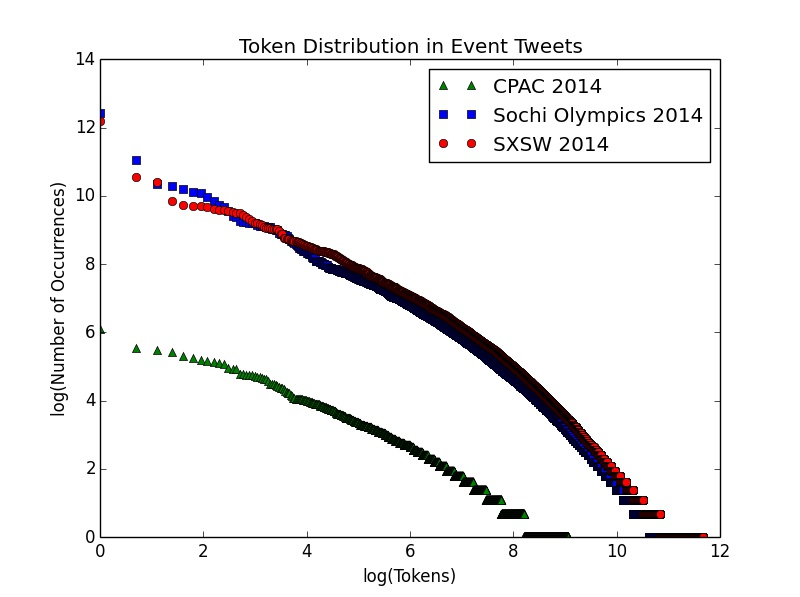
\includegraphics[width=14cm,height=11cm]{Figures/TokenDistribution.jpeg}
\end{figure}

\begin{figure}[htbp]
  \caption{Distribution of URLs in event related tweets.}
\label{urldist}
  \centering
    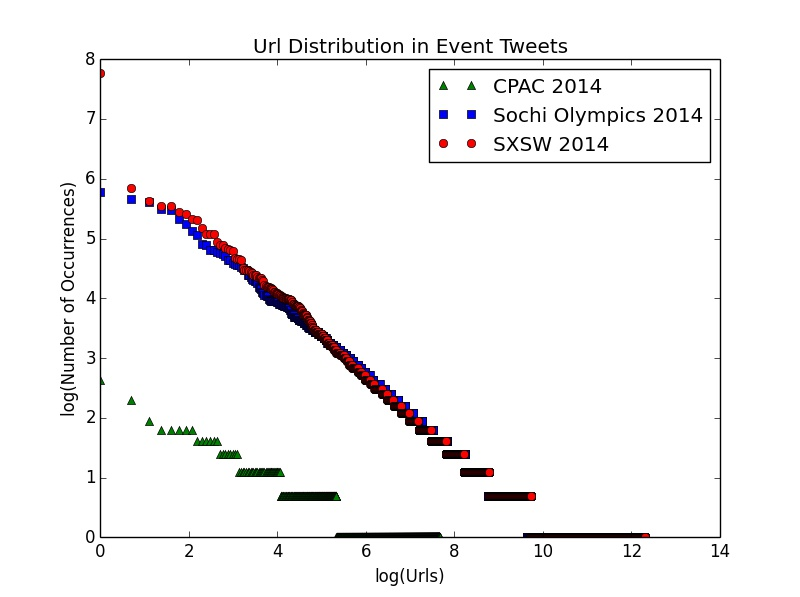
\includegraphics[width=14cm,height=11cm]{Figures/UrlDistribution.jpeg}
\end{figure}

\begin{figure}[htbp]
  \caption{Distribution of users in event related tweets.}
\label{userdist}
  \centering
    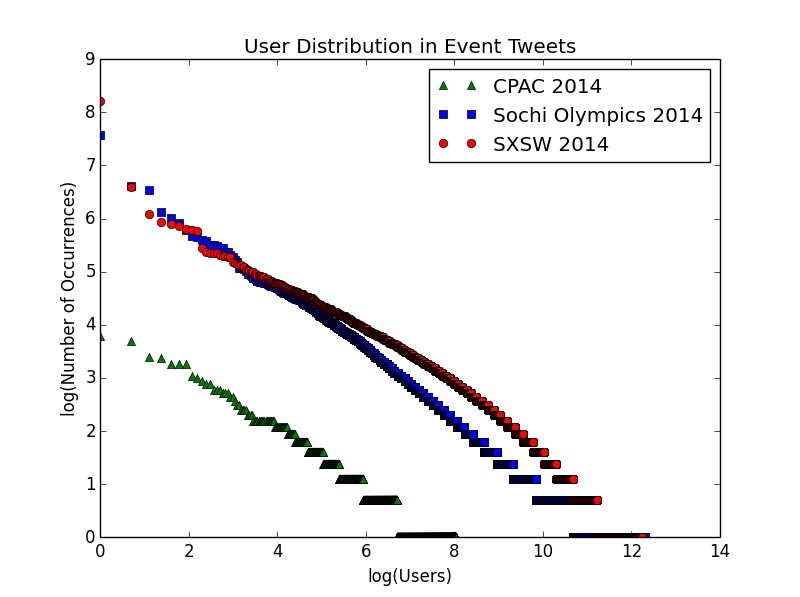
\includegraphics[width=14cm,height=11cm]{Figures/UserDistribution.jpeg}
\end{figure}



Our second step was to use the logistic regression model developed for the `Event Information Quality' component and assign informativeness scores to all the 3.8 million tweets in the dataset. The tweets getting a score greater than 0.7 were considered as instances of high quality informative tweets. Those getting a score lesser than 0.3 were considered as instances of low quality non-informative tweets. We calculated the average values of different content characteristics of the tweets. Top ten percent of the frequently occurring hashtags and nouns were considered as top hashtags and top nouns respectively, for the analysis. Some of the characteristics that were prominently different for informative and non-informative tweets are listed in Table \ref{infoanalysis}.

\begin{figure}[htbp]
\centering
\caption{Content characteristics of informative and non-informative tweets related to events.}
    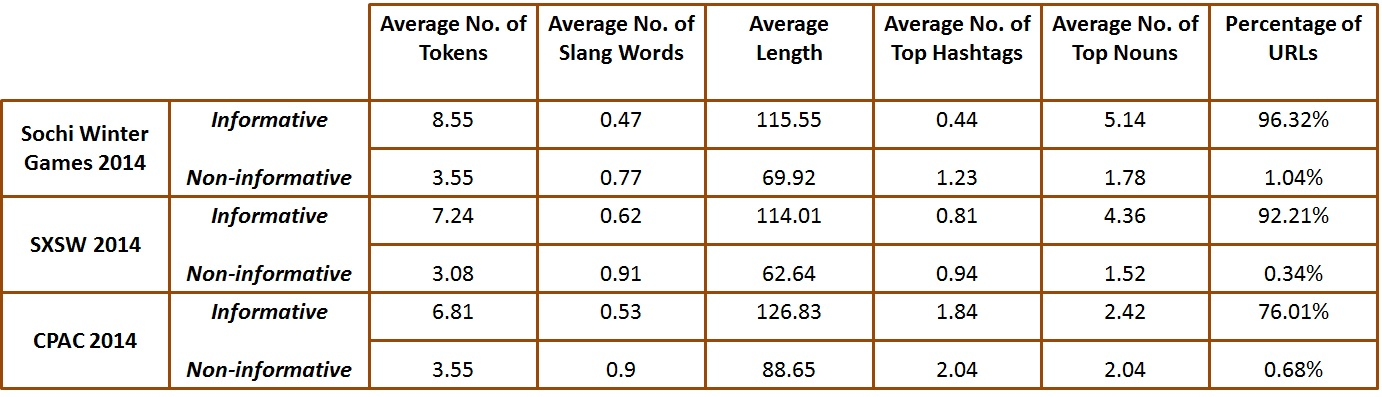
\includegraphics[width=15cm,height=5cm]{Figures/InformationAnalysisTable.jpg}
    
    \label{infoanalysis}
\end{figure}

As presented in the table, some of the observations for all the three events are, 

\begin{itemize}
\item On an average the informative tweets are marked by a higher number of tokens per tweet and greater occurrence of top nouns. 
\item The average length of informative tweets is also more than the non-informative ones. 
\item The percentage of informative tweets having URLs is strikingly high. 
\item A greater use of slang words is observed in non-informative tweets. 
\item Greater occurrence of top hashtags in non-informative tweets intrigued us to look into the content and obtain a detailed view of it. We observed that a lot of non-informative tweets have used popular hashtags with unrelated content and URLs directing to irrelevant information. This is typical of spam tweets as already pointed out in Chapter \ref{challenges}, Section \ref{veracity}. 
\item The average number of follower counts for users posting informative tweets was also observed to be higher than the ones posting non-informative ones. 
\item The average number of feeling words used in informative tweets were also relatively higher than the feeling words used in the non-informative tweets. 
\end{itemize}

The above observations gave us an idea of how high quality informative content related to events is produced in Twitter and the characteristics that differentiate them from low quality non-informative content. We made the following conclusions based on the observations:
\begin{itemize}
\item It is now intuitive that the informative tweets are more expressive, formal and lengthier, marked by higher presence of nouns. 
\item The high presence of nouns indicates that these tweets also contain information about people, places, organizations, etc, associated with the events, which is vital information about any event and is ideal for representing its identity. 
\item Due to the limitations imposed by Twitter on the number of characters in a tweet, the users tend to share URLs along with the textual content that might lead to more information about the event. 
\item Also, users with high follower counts tend to post informative tweets. This can also be concluded by the fact that as they have more followers they are encouraged to share informative content. Conversely, since they share informative content they are followed by a large number of other users interested in the content shared by them.
\end{itemize}

\subsection{Event Identity Information Units}
After the observations in the previous section we conclude that the informative tweets in general are characterized by wordiness, occurrences of URLs and are posted by users with high follower count. These characteristics are also the primary features that distinguish informative from non-informative content. Although, presence of hashtags is not a good indicator of informativeness, yet it is a strong identifier of a topic as already pointed by \cite{laniado2010making}. Popular hashtags for an event might be used maliciously. On the other hand, the presence of a popular hashtag in a wordy tweet consisting of words popular for the event, along with a popular URL, posted by an influential user is highly likely to contain event-specific content. Therefore, it is intuitive that given a stream of tweets for an event an optimal combination of event related popular text units (words, unigrams, bigrams etc),  hashtags, and URLs, posted by an influential user in a tweet, is one of the key indicators for identifying event-specific informative content. It would be highly unlikely for a tweet to contain all of these and yet not convey useful event-specific information. Based on the above analysis we decided to build the EIIS for an event $E_{i}$, composed of the following event identity information units:

\begin{enumerate}
\item A set of tweets $M_{E_{i}} = {\{m_{1_{E_{i}}},m_{2_{E_{i}}}, ... ,m_{n_{E_{i}}}\}}$, related to the event $E_{i}$, having high chances of containing informative content.
\item A set of hashtags $H_{E_{i}} = \{h_{1_{E_{i}}},h_{2_{E_{i}}},..., h_{p_{E_{i}}} \}$, used for annotating the tweets ($\in M_{E_{i}}$) related to event $E_{i}$.
\item A set of text units $W_{E_{i}} = \{w_{1_{E_{i}}},w_{2_{E_{i}}},..., w_{r_{E_{i}}} \}$, used for expressing textual content in tweets ($\in M_{E_{i}}$), related to event $E_{i}$.
\item A set of URLs $L_{E_{i}} = \{l_{1_{E_{i}}},l_{2_{E_{i}}},..., l_{t_{E_{i}}} \}$, shared in the tweets ($\in M_{E_{i}}$) related to event $E_{i}$.
\item A set of users $U_{E_{i}} = \{u_{1_{E_{i}}},u_{2_{E_{i}}},..., u_{s_{E_{i}}} \}$, tweeting the tweets ($\in M_{E_{i}}$), about the event $E_{i}$.
\end{enumerate}

\subsection{Extracting Event Identity Information Units}
The event identity information units for an event $E_{i}$, as defined above are extracted from the event dataset. Following steps are taken:
\begin{itemize}
\item A threshold for the informativeness score assigned in the previous component is set between 0.0-1.0, for extracting the tweets ($\in M_{E_{i}}$). We set a threshold of 0.7. Therefore, the tweets having an informativeness score greater than or equal to 0.7 are filtered out and comprises the set $M_{E_{i}}$.
\item The hashtags that were extracted in the `Event Reference Preparation' step from the tweets $\in M_{E_{i}}$, are used for populating the set $H_{E_{i}}$. However, the hashtags that matches the slang words and stop words are not considered. This is done in order to ensure good quality of information contextualized by the hashtags.
\item The nouns that were extracted in the `Event Reference Preparation' step from the tweets $\in M_{E_{i}}$, are considered as the text units ($\in W_{E_{i}}$). The nouns that matches the slang words are not considered. This is done in order to ensure good quality of textual content represented by the nouns. In another experiment, we considered the extracted named entities as the text units. We report our results and compare the results obtained in both the cases in the next Chapter.
\item The expanded URLs from the meta-data of the tweets $\in M_{E_{i}}$ populates the set $L_{E_{i}}$.
\item The meta-information of the users posting the tweets $\in M_{E_{i}}$, represented by their user ids, is extracted for populating the set $U_{E_{i}}$ 
\end{itemize}  

These event identity information units forms the Event Identity Information Structure (EIIS), as explained next.

\section{Event Identity Information Structure (EIIS)}
This is the component that maintains a persistent EIIS as introduced in Chapter \ref{events}, Section \ref{problem}, for each individual event tracked by the framework and updates the metadata of the EIIS throughout the EIIM life cycle. Due to the unstructured nature of the social media references and evolving nature of the events, we store the event identity information units extracted by the previous component along with their associated meta-data, in a persistent graph data structure stored in the database. We update the meta-data related to each node of the graph using the normal database updation queries. Adjacency lists are used for representing the graph. The choice of storing the event identity information units in a graph structure is also motivated by the wide array of graph processing algorithms used for natural language processing and text mining operations. We show the efficacy and the advantages of a graph in the next section. 

\begin{itemize}
\item Therefore the EIIS is a graph $\mathbf{G_{E_{i}} = (V_{E_{i}},D_{E_{i}})}$, where $\mathbf{V_{E_{i}} = M_{E_{i}} \cup H_{E_{i}} \cup W_{E_{i}} \cup U_{E_{i}} \cup}$ \\  $\mathbf{L_{E_{i}}}$, is the set of vertices and $\mathbf{D_{E_{i}}}$ is the set of directed edges between different vertices. Whenever two vertices are associated, there are two edges between them that are oppositely directed. For example, if a tweets consist of hashtags, text units, URLs and is posted by an user, then there are bi-directed edges between each one of them. 
\end{itemize}




\begin{figure}[htbp]
  \caption{Event Identity Information Structure component of the EIIM life cycle.}
  \centering
    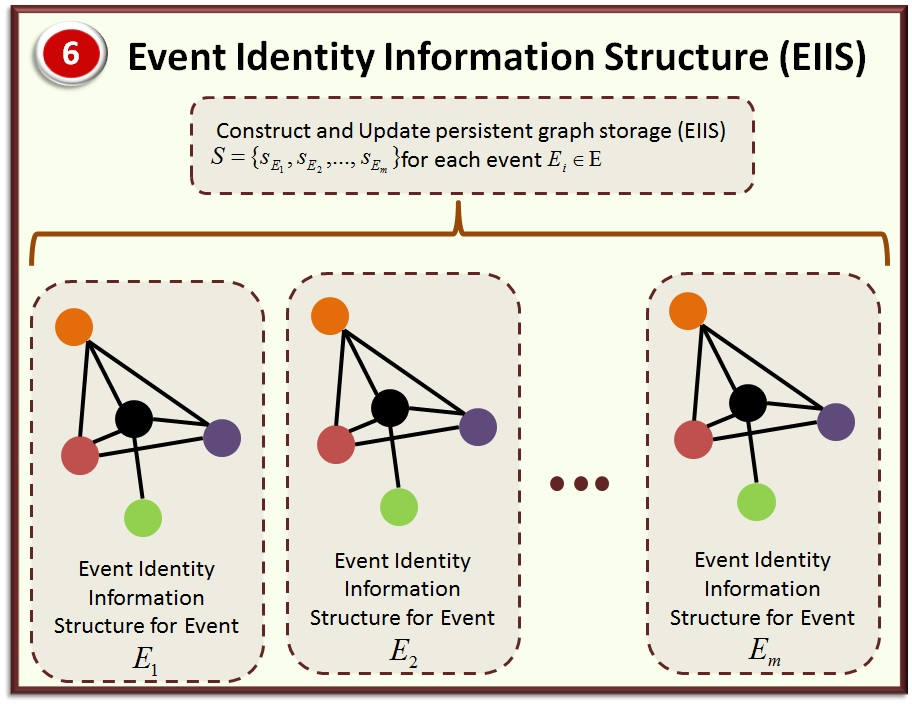
\includegraphics[width=14cm,height=11cm]{Figures/EIIS.jpg}
\end{figure}


\begin{figure}[htbp]
  \caption{Event Identity Information Processing component of the EIIM life cycle.}
  \centering
    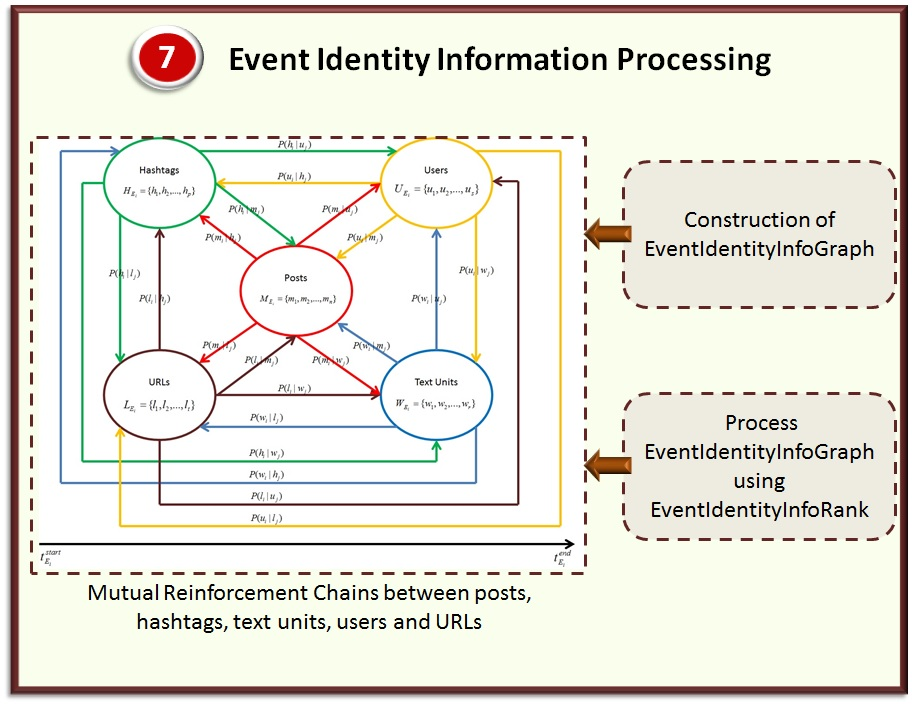
\includegraphics[width=14cm,height=11cm]{Figures/EIIMComponents/EventIdentityInformationProcessing.jpg}
\end{figure}

\section{Event Identity Information Processing\label{EventIdentityInformationProcessing}}
This is the most important processing component of the EIIM life cycle and is at the heart of the entire framework. We make our most novel contributions in this component. The component is mainly divided into two sub-components:
\begin{itemize}
\item \textbf{EventIdentityInfoGraph} - that represents and defines novel relationships between the vertices of the graph $\mathbf{G}$ representing the EIIS.
\item \textbf{EventIdentityInfoProcess} - processes the \textit{EventIdentityInfoGraph} in order to rank its nodes and identify the top most informative event identity information units that acts as inputs to the next two components of the EIIM life cycle.
\end{itemize}

\subsection{EventIdentityInfoGraph\label{eventidentityinfograph}}

We implement a novel graph structure - \textit{EventIdentityInfoGraph}, which is dynamically generated from the graph $\mathbf{G}$ (EIIS), after a configurable interval of time, using following assumptions.
  
For an event $E_{i}$ 
\begin{itemize} 
\item a \textit{tweet is an event-specific informative tweet} if it is strongly associated with:
\begin{itemize}
\item[\textbf{(a)}] \textit{event-specific informative hashtags}, 
\item[\textbf{(b)}] \textit{event-specific informative text units}, 
\item[\textbf{(c)}] \textit{event-specific informative users},
\item[\textbf{(d)}] \textit{event-specific informative URLs}. 
\end{itemize}
\end{itemize}

\begin{itemize} 
\item a \textit{hashtag is an event-specific informative hashtag} if it is strongly associated with:
\begin{itemize}
\item[\textbf{(a)}] \textit{event-specific informative tweets},
\item[\textbf{(b)}] \textit{event-specific informative text units},
\item[\textbf{(c)}] \textit{event-specific informative users},
\item[\textbf{(d)}] \textit{event-specific informative URLs}.
\end{itemize}
\end{itemize}

\begin{itemize} 
\item a \textit{text unit is an event-specific informative text unit} if it is strongly associated with:
\begin{itemize}
\item[\textbf{(a)}] \textit{event-specific informative tweets}, 
\item[\textbf{(b)}] \textit{event-specific informative hashtags}, 
\item[\textbf{(c)}] \textit{event-specific informative users}, 
\item[\textbf{(d)}] \textit{event-specific informative URLs}. 
\end{itemize}
\end{itemize}

\begin{itemize} 
\item a \textit{user is an event-specific informative user} if it is strongly associated with:
\begin{itemize}
\item[\textbf{(a)}] \textit{event-specific informative tweets}, 
\item[\textbf{(b)}] \textit{event-specific informative hashtags}, 
\item[\textbf{(c)}] \textit{event-specific informative text units},
\item[\textbf{(d)}] \textit{event-specific informative URLs}. 
\end{itemize}
\end{itemize}

\begin{itemize} \item a \textit{URL is an event-specific informative URL} if it is strongly associated with:
\begin{itemize}
\item[\textbf{(a)}] \textit{event-specific informative tweets}, 
\item[\textbf{(b)}] \textit{event-specific informative hashtags}, 
\item[\textbf{(c)}] \textit{event-specific informative text units},
\item[\textbf{(d)}] \textit{event-specific informative users}. 
\end{itemize}
\end{itemize}

%\end{itemize}

The relationships for an event $E_{i}$ as stated above, forms a \textit{Mutual Reinforcement Chain} \cite{wei2008query} for the event $E_{i}$ as shown in Figure \ref{mrc}. We represent this relationship in a graph $\mathbf{G_{E_{i}(t)} = (V_{E_{i}(t)},D_{E_{i}(t)})}$, which we call as \textit{EventIdentityInfoGraph}, where $V_{E_{i}(t)} = M_{E_{i}} \cup H_{E_{i}} \cup W_{E_{i}} \cup U_{E_{i}} \cup L_{E_{i}}$, is the set of vertices and $\mathbf{D_{E_{i}(t)}}$ is the set of directed edges between different vertices. The graph $G_{E_{i}(t)}$ is basically, a snapshot of the EIIS structure of the event $E_{i}$ at time t. 

\begin{figure}[htbp]
\centering
\caption{\small Mutual Reinforcement Chains in Twitter for an event.}    
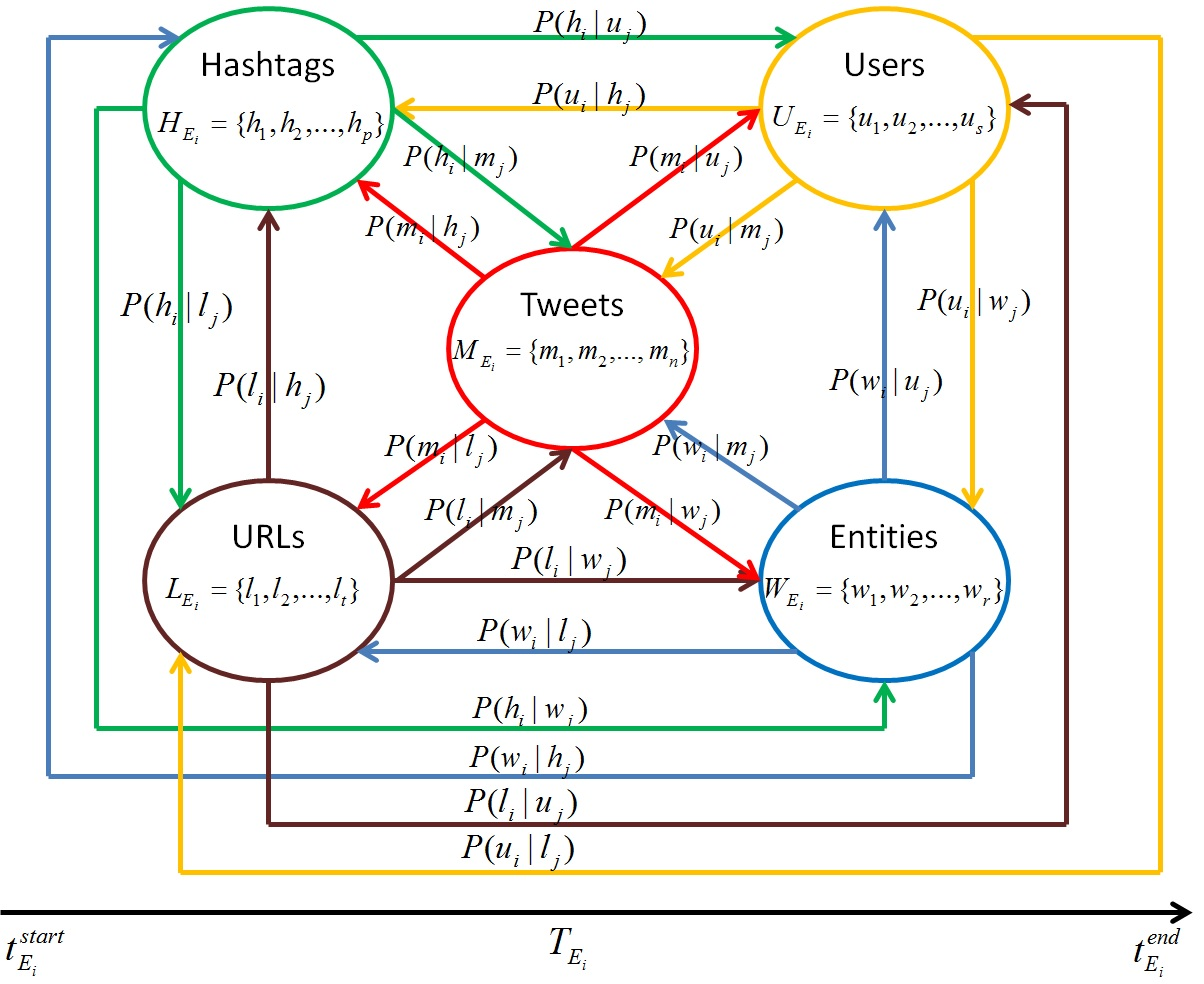
\includegraphics[width=16cm,height=12cm]{Figures/TwitterEventInfoGraph.jpg}
\label{mrc}
\end{figure}
 

Whenever two vertices are associated, there are two edges between them that are oppositely directed. Each directed edge is assigned a weight, which determines the degree of association of one vertex with the other. The weights for each edge is calculated according to the conditional probabilities as given by equations 5.1-5.18. 

\begin{equation}
P(h_{i_{E_{i}}} \mid w_{j_{E_{i}}}) = \frac{No. \, of \, tweets \, h_{i_{E_{i}}} \, and \, w_{j_{E_{i}}} \, occur \, together}{No. \, of \, tweets \, w_{j_{E_{i}}} \, occurs}
\end{equation}

\begin{equation}
P(w_{i_{E_{i}}} \mid h_{j_{E_{i}}}) = \frac{No. \, of \, tweets \, w_{i_{E_{i}}} \, and \, h_{j_{E_{i}}} \, occur \, together}{No. \, of \, tweets \, h_{j_{E_{i}}} \, occurs}
\end{equation}

\begin{equation}
P(h_{i_{E_{i}}} \mid l_{j_{E_{i}}}) = \frac{No. \, of \, tweets \, h_{i_{E_{i}}} \, and \, l_{j_{E_{i}}} \, occur \, together}{No. \, of \, tweets \, l_{j_{E_{i}}} \, occurs}
\end{equation}

\begin{equation}
P(l_{i_{E_{i}}} \mid h_{j_{E_{i}}}) = \frac{No. \, of \, tweets \, l_{i_{E_{i}}} \, and \, h_{j_{E_{i}}} \, occur \, together}{No. \, of \, tweets  \, h_{j_{E_{i}}} \, occurs}
\end{equation}

\begin{equation}
P(h_{i_{E_{i}}} \mid u_{j_{E_{i}}}) = \frac{No. \, of \, tweets  \, h_{i_{E_{i}}} \, and \, u_{j_{E_{i}}} \, occur \, together}{No. \, of \, tweets  \, u_{j_{E_{i}}} \, occurs}
\end{equation}

\begin{equation}
P(u_{i_{E_{i}}} \mid h_{j_{E_{i}}}) = \frac{No. \, of \, tweets  \, u_{i_{E_{i}}} \, and \, h_{j_{E_{i}}} \, occur \, together}{No. \, of \, tweets  \, h_{j_{E_{i}}} \, occurs}
\end{equation}

\begin{equation}
P(w_{i_{E_{i}}} \mid l_{j_{E_{i}}}) = \frac{No. \, of \, tweets  \, w_{i_{E_{i}}} \, and \, l_{j_{E_{i}}} \, occur \, together}{No. \, of \, tweets  \, l_{j_{E_{i}}} \, occurs}
\end{equation}

\begin{equation}
(l_{i_{E_{i}}} \mid w_{j_{E_{i}}}) = \frac{No. \, of \, tweets  \, l_{i_{E_{i}}} \, and \, w_{j_{E_{i}}} \, occur \, together}{No. \, of \, tweets  \, w_{j_{E_{i}}} \, occurs}
\end{equation}

\begin{equation}
P(u_{i_{E_{i}}} \mid l_{j_{E_{i}}}) = \frac{No. \, of \, tweets  \, u_{i_{E_{i}}} \, and \, l_{j_{E_{i}}} \, occur \, together}{No. \, of \, tweets  \, l_{j_{E_{i}}} \, occurs}
\end{equation}

\begin{equation}
P(l_{i_{E_{i}}} \mid u_{j_{E_{i}}}) = \frac{No. \, of \, tweets  \, l_{i_{E_{i}}} \, and \, u_{j_{E_{i}}} \, occur \, together}{No. \, of \, tweets  \, u_{j_{E_{i}}} \, occurs}
\end{equation}

\begin{equation}
P(h_{i_{E_{i}}} \mid m_{j_{E_{i}}}) = 1.0
\end{equation}

\begin{equation}
P(m_{i_{E_{i}}} \mid h_{j_{E_{i}}}) = 1.0
\end{equation}

\begin{equation}
P(w_{i_{E_{i}}} \mid m_{j_{E_{i}}}) = 1.0
\end{equation}

\begin{equation}
P(m_{i_{E_{i}}} \mid w_{j_{E_{i}}}) = 1.0
\end{equation}

\begin{equation}
P(u_{i_{E_{i}}} \mid m_{j_{E_{i}}}) = 1.0
\end{equation}

\begin{equation}
P(m_{i_{E_{i}}} \mid u_{j_{E_{i}}}) = 1.0
\end{equation}

\begin{equation}
P(l_{i_{E_{i}}} \mid m_{j_{E_{i}}}) = 1.0
\end{equation}

\begin{equation}
P(m_{i_{E_{i}}} \mid l_{j_{E_{i}}}) = 1.0
\end{equation}


We do not consider an edge between two vertices of same type. That is, we don't connect a tweet with another tweet. Similarly, for hashtags, text units, users and URLs. This constraint was imposed in order to deal with the nepotistic relationships between high quality content and low quality content introduced by the malicious users for promoting the low quality content as explained in Chapter \ref{challenges}, Section \ref{veracity}.  



%\begin{table*}[ht]
%\caption{Affinity scores of edges between vertices of TwitterEventInfoGraph}
%\label{edgescores}
%\begin{tabular}{|l|}
%\hline 
%\underline{\textbf{\textit{Affinity scores (edge weights) between different vertices}} $\in M_{E_{i}}, H_{E_{i}}, W_{E_{i}}, U_{E_{i}},$} \\ \underline{\textbf{\textit{$L_{E_{i}}$:}}} \\ \\
%$P(h_{i} \mid w_{j}) = \frac{No. \, of \, tweets \, h_{i} \, and \, w_{j} \, occur \, together}{No. \, of \, tweets \, w_{j} \, occurs}$, $P(w_{i} \mid h_{j}) = \frac{No. \, of \, tweets \, w_{i} \, and \, h_{j} \, occur \, together}{No. \, of \, tweets \, h_{j} \, occurs}$, \\
%
%
%$P(h_{i} \mid l_{j}) = \frac{No. \, of \, tweets \, h_{i} \, and \, l_{j} \, occur \, together}{No. \, of \, tweets \, l_{j} \, occurs}$,
%$P(l_{i} \mid h_{j}) = \frac{No. \, of \, tweets \, l_{i} \, and \, h_{j} \, occur \, together}{No. \, of \, tweets  \, h_{j} \, occurs}$, \\
%
%$P(h_{i} \mid u_{j}) = \frac{No. \, of \, tweets  \, h_{i} \, and \, u_{j} \, occur \, together}{No. \, of \, tweets  \, u_{j} \, occurs}$,
%$P(u_{i} \mid h_{j}) = \frac{No. \, of \, tweets  \, u_{i} \, and \, h_{j} \, occur \, together}{No. \, of \, tweets  \, h_{j} \, occurs}$,  \\
%
%$P(w_{i} \mid l_{j}) = \frac{No. \, of \, tweets  \, w_{i} \, and \, l_{j} \, occur \, together}{No. \, of \, tweets  \, l_{j} \, occurs}$, 
%$P(l_{i} \mid w_{j}) = \frac{No. \, of \, tweets  \, l_{i} \, and \, w_{j} \, occur \, together}{No. \, of \, tweets  \, w_{j} \, occurs}$, \\ 
%
%$P(w_{i} \mid u_{j}) = \frac{No. \, of \, tweets  \, w_{i} \, and \, u_{j} \, occur \, together}{No. \, of \, tweets  \, u_{j} \, occurs}$,
%$P(u_{i} \mid w_{j}) = \frac{No. \, of \, tweets  \, u_{i} \, and \, w_{j} \, occur \, together}{No. \, of \, tweets  \, w_{j} \, occurs}$, \\
%
%$P(u_{i} \mid l_{j}) = \frac{No. \, of \, tweets  \, u_{i} \, and \, l_{j} \, occur \, together}{No. \, of \, tweets  \, l_{j} \, occurs}$, 
%$P(l_{i} \mid u_{j}) = \frac{No. \, of \, tweets  \, l_{i} \, and \, u_{j} \, occur \, together}{No. \, of \, tweets  \, u_{j} \, occurs}$, \\
%
%
%$P(h_{i} \mid m_{j}) = P(m_{i} \mid h_{j}) = P(w_{i} \mid m_{j}) = P(m_{i} \mid w_{j}) = P(u_{i} \mid m_{j}) = P(m_{i} \mid u_{j}) =$ \\ $P(l_{i} \mid m_{j})= P(m_{i} \mid l_{j})= 1.0$  \\ \\ 
%\textbf{Note:} $P(h_{i} \mid w_{j})$ should be read as the probability of occurrence of hashtag $h_{i}$ given \\ the occurrence of the text unit $w_{j}$ in the stream of  tweets $M_{E_{i}}$ related to event $E_{i}$ \\ collected over the time period $T_{E_{i}}$. Similarly, for others.\\
%\hline 
%\end{tabular}
%\end{table*}










Next, we explain \textit{EventIdentityInfoRank}.

%%%%%%%%%%%%%%%%%%%%%%%%%%%%%%%%%%%%%%%%%%%%%%%%%%%%%%%%%%%%%%%%%%%%%%%%%%%%%%%%%%
%%%%%%%%%%%%%%%%%                                       TwitterEventInfoRank Subsection                    %%%%%%%%%%%%%%%%%%%%%%%%%%%%%%%%%%
%%%%%%%%%%%%%%%%%%%%%%%%%%%%%%%%%%%%%%%%%%%%%%%%%%%%%%%%%%%%%%%%%%%%%%%%%%%%%%%%%%

\subsection{EventIdentityInfoRank\label{eventidentityinforank}}
\textit{EventIdentityInfoRank} is an iterative algorithm that takes into account the mutually reinforcing relationships between the vertices of \textit{EventIdentityInfoGraph} as explained in the previous section and propagates event-specific scores of each vertex to connected vertices across the graph for ranking its vertices ($\in V_{E_{i}(t)}$) in terms of event-specific informativeness.

We first assign a event-specific score to all the vertices of the graph. Event-specific scores for vertices $(\in H_{E_{i}}, W_{E_{i}}, U_{E_{i}}, L_{E_{i}})$ are calculated using equations 5.19-5.22. The tweets  $(\in M_{E_{i}})$ are assigned an initial informativeness score as obtained from the logistic regression model in `Event Information Quality' component. The event-specific scores for vertices $(\in H_{E_{i}}, W_{E_{i}}, U_{E_{i}}, L_{E_{i}})$ and informativeness score for vertices $(\in M_{E_{i}})$ gives an initial ranking of all the vertices of \textit{EventIdentityInfoGraph}. We aim to refine the initial scores and assign a final score for ranking the vertices by leveraging the mutually reinforcing relationships between them.
\begin{equation}
Score(h_{i_{E_{i}}}) = \frac{freq(h_{i})}{max\{freq(h_{1}),freq(h_{2}),...,freq(h_{p})\}}
\end{equation}

\begin{equation}
Score(w_{i_{E_{i}}}) = \frac{freq(w_{i})}{max\{freq(w_{1}),freq(w_{2}),...,freq(w_{r})\}}
\end{equation}

\begin{equation}
Score(u_{i_{E_{i}}}) = \frac{followers(u_{i})}{max\{followers(u_{1}),...,followers(u_{r})\}}
\end{equation}

\begin{equation}
Score(l_{i_{E_{i}}}) = \frac{freq(l_{i})}{max\{freq(l_{1}),freq(l_{2}),...,freq(l_{r})\}}
\end{equation}


The relationships between two different subsets of vertices in graph $\mathbf{G_{E_{i}(t)}}$ is denoted by an affinity matrix. For e.g., $\mathbf{A_{E_{i}}^{MH}}$ denotes the $\mathbf{M_{E_{i}}-H_{E_{i}}}$ affinity matrix for event $E_{i}$, where $\mathbf{(i,j)^{th}}$ entry is the edge weight quantifying the association between $i^{th}$ tweet ($\in M_{E_{i}}$) and $j^{th}$ hashtag ($\in H_{E_{i}}$), calculated using equations 5.1-5.18. Similarly, $\mathbf{A_{E_{i}}^{WH}}$ denotes the $\mathbf{W_{E_{i}}-H_{E_{i}}}$ affinity matrix between set of text units $W_{E_{i}}$ and set of hashtags $H_{E_{i}}$ for event $E_{i}$, and so on.


The rankings of \textit{tweets}, \textit{hashtags}, \textit{text units}, \textit{users} and \textit{URLs} in terms of event-specific informativeness, can be iteratively derived from the Mutual Reinforcement Chain for the event. Let $R_{{E_{i}}}^{M}$, $R_{{E_{i}}}^{H}$, $R_{{E_{i}}}^{W}$, $R_{{E_{i}}}^{U}$ and $R_{{E_{i}}}^{L}$ denote the ranking scores for the set of tweets ($\in M_{E_{}}$), set of  hashtags $(\in H_{E_{i}})$, set of text units $(\in W_{E_{i}})$, set of users $(\in U_{E_{i}})$, and set of URLs $(\in L_{E_{i}})$, respectively. Therefore, the Mutual Reinforcement Chain ranking for the $k^{th}$ iteration can be formulated as follows:
 

%\begin{equation}
%\tiny R_{{E_{i}}}^{M(k+1)} = A_{E_{i}}^{MM(k)}R_{{E_{i}}}^{M(k)} + A_{E_{i}}^{MH(k)}R_{{E_{i}}}^{H(k)} + A_{E_{i}}^{MW(k)}R_{{E_{i}}}^{W(k)} + A_{E_{i}}^{MU(k)}R_{{E_{i}}}^{U(k)} + A_{E_{i}}^{ML(k)}R_{{E_{i}}}^{L(k)}
%\end{equation}

\begin{equation}
R_{{E_{i}}}^{M(k+1)} = A_{E_{i}}^{MM(k)}R_{{E_{i}}}^{M(k)} + A_{E_{i}}^{MH(k)}R_{{E_{i}}}^{H(k)} + A_{E_{i}}^{MW(k)}R_{{E_{i}}}^{W(k)}+ A_{E_{i}}^{MU(k)}R_{{E_{i}}}^{U(k)} + A_{E_{i}}^{ML(k)}R_{{E_{i}}}^{L(k)}
\end{equation}

%\begin{equation}
%\tiny R_{{E_{i}}}^{H(k+1)} = A_{E_{i}}^{HM(k)}R_{{E_{i}}}^{M(k)} + A_{E_{i}}^{HH(k)}R_{{E_{i}}}^{H(k)} + A_{E_{i}}^{HW(k)}R_{{E_{i}}}^{W(k)} + A_{E_{i}}^{HU(k)}R_{{E_{i}}}^{U(k)} + A_{E_{i}}^{HL(k)}R_{{E_{i}}}^{L(k)}
%\end{equation}

\begin{equation}
R_{{E_{i}}}^{H(k+1)} = A_{E_{i}}^{HM(k)}R_{{E_{i}}}^{M(k)} + A_{E_{i}}^{HH(k)}R_{{E_{i}}}^{H(k)} + A_{E_{i}}^{HW(k)}R_{{E_{i}}}^{W(k)}+ A_{E_{i}}^{HU(k)}R_{{E_{i}}}^{U(k)} + A_{E_{i}}^{HL(k)}R_{{E_{i}}}^{L(k)}
\end{equation}



%\begin{equation}
%\tiny R_{{E_{i}}}^{W(k+1)} = A_{E_{i}}^{WM(k)}R_{{E_{i}}}^{M(k)} + A_{E_{i}}^{WH(k)}R_{{E_{i}}}^{H(k)} + A_{E_{i}}^{WW(k)}R_{{E_{i}}}^{W(k)} + A_{E_{i}}^{WU(k)}R_{{E_{i}}}^{U(k)} + A_{E_{i}}^{WL(k)}R_{{E_{i}}}^{L(k)}
%\end{equation}

\begin{equation}
R_{{E_{i}}}^{W(k+1)} = A_{E_{i}}^{WM(k)}R_{{E_{i}}}^{M(k)} + A_{E_{i}}^{WH(k)}R_{{E_{i}}}^{H(k)} + A_{E_{i}}^{WW(k)}R_{{E_{i}}}^{W(k)}+ A_{E_{i}}^{WU(k)}R_{{E_{i}}}^{U(k)} + A_{E_{i}}^{WL(k)}R_{{E_{i}}}^{L(k)}
\end{equation}

%\begin{equation}
%\tiny R_{{E_{i}}}^{U(k+1)} = A_{E_{i}}^{UM(k)}R_{{E_{i}}}^{M(k)} + A_{E_{i}}^{UH(k)}R_{{E_{i}}}^{H(k)} + A_{E_{i}}^{UW(k)}R_{{E_{i}}}^{W(k)} + A_{E_{i}}^{UU(k)}R_{{E_{i}}}^{U(k)} + A_{E_{i}}^{UL(k)}R_{{E_{i}}}^{L(k)}
%\end{equation}

\begin{equation}
R_{{E_{i}}}^{U(k+1)} = A_{E_{i}}^{UM(k)}R_{{E_{i}}}^{M(k)} + A_{E_{i}}^{UH(k)}R_{{E_{i}}}^{H(k)} + A_{E_{i}}^{UW(k)}R_{{E_{i}}}^{W(k)}+ A_{E_{i}}^{UU(k)}R_{{E_{i}}}^{U(k)} + A_{E_{i}}^{UL(k)}R_{{E_{i}}}^{L(k)}
\end{equation}

%\begin{equation}
%\tiny R_{{E_{i}}}^{L(k+1)} = A_{E_{i}}^{LM(k)}R_{{E_{i}}}^{M(k)} + A_{E_{i}}^{LH(k)}R_{{E_{i}}}^{H(k)} + A_{E_{i}}^{LW(k)}R_{{E_{i}}}^{W(k)} + A_{E_{i}}^{LU(k)}R_{{E_{i}}}^{U(k)} + A_{E_{i}}^{LL(k)}R_{{E_{i}}}^{L(k)}
%\end{equation}


\begin{equation}
R_{{E_{i}}}^{L(k+1)} = A_{E_{i}}^{LM(k)}R_{{E_{i}}}^{M(k)} + A_{E_{i}}^{LH(k)}R_{{E_{i}}}^{H(k)} +A_{E_{i}}^{LW(k)}R_{{E_{i}}}^{W(k)}+ A_{E_{i}}^{LU(k)}R_{{E_{i}}}^{U(k)}+ A_{E_{i}}^{LL(k)}R_{{E_{i}}}^{L(k)}
\end{equation}


The equations 5-9 can be represented in the form of a block matrix $\Delta_{E_{i}}$, where,
\[ \Delta_{E_{i}} = \left( \begin{array}{ccccc}
A_{E_{i}}^{MM} & A_{E_{i}}^{MH} & A_{E_{i}}^{MW} &  A_{E_{i}}^{MU} & A_{E_{i}}^{ML} \\
A_{E_{i}}^{HM} & A_{E_{i}}^{HH} & A_{E_{i}}^{HW} & A_{E_{i}}^{HU} & A_{E_{i}}^{HL} \\
A_{E_{i}}^{WM} & A_{E_{i}}^{WH} & A_{E_{i}}^{WW} & A_{E_{i}}^{WU} & A_{E_{i}}^{WL}\\
A_{E_{i}}^{UM} & A_{E_{i}}^{UH} & A_{E_{i}}^{UW} & A_{E_{i}}^{UU} & A_{E_{i}}^{UL} \\
A_{E_{i}}^{LM} & A_{E_{i}}^{LH} & A_{E_{i}}^{LW} & A_{E_{i}}^{LU} & A_{E_{i}}^{LL} \end{array} \right)\] 

Let \[R_{E_{i}} = \left( \begin{array}{c}
R_{{E_{i}}}^{M} \\
R_{{E_{i}}}^{H} \\
R_{{E_{i}}}^{W} \\
R_{{E_{i}}}^{U} \\
R_{{E_{i}}}^{L} \end{array} \right)\] 

then, $R_{E_{i}}$ can be computed as the dominant eigenvector of $\Delta_{E_{i}}$.
\begin{equation}
\Delta_{E_{i}}.R_{E_{i}} = \lambda.R_{E_{i}}
\end{equation}

In order to guarantee a unique $R_{E_{i}}$, $\Delta_{E_{i}}$ must be forced to be stochastic and irreducible. 

To make $\Delta_{E_{i}}$ stochastic we divide the value of each element in a column of $\Delta_{E_{i}}$ by the sum of the values of all the elements in that column. This finally makes $\Delta_{E_{i}}$ column stochastic. We now denote it by $\hat \Delta_{E_{i}}$.
%we remove all the rows and columns of the block matrices whose all elements are zeros. Since, we don't consider edges between two vertices of same type, all the elements of the diagonal block matrices are zero by default. We then 

Next, we make $\hat \Delta_{E_{i}}$ irreducible. This is done by making the graph $G$ strongly connected by adding links from one node to any other node with a probability vector $p$. Now, $\hat \Delta_{E_{i}}$ is transformed to 

\begin{equation}
\overline \Delta_{E_{i}} = \alpha \hat \Delta_{E_{i}} + (1-\alpha)E
\end{equation}
\begin{equation}
E = p \times [1]_{1 \times k}
\end{equation}
where $0 \le \alpha \le 1$ is set to 0.85 according to \textit{PageRank}, and k is the order of $\hat \Delta_{E_{i}}$. We set $p = [1/k]_{k \times 1}$ by assuming a uniform distribution over all elements. Now, $\overline \Delta_{E_{i}}$ is stochastic and irreducible and it can be shown that it is also primitive by checking $\overline \Delta_{E_{i}}^{2}$ is greater than $0$.

Following steps are taken next,
\begin{itemize}
\item[\textbf{1.}] We initialize the rank vectors ($ R_{{E_{i}}}^{M(0)}, R_{{E_{i}}}^{H(0)}, R_{{E_{i}}}^{W(0)}, R_{{E_{i}}}^{U(0)}, R_{{E_{i}}}^{L(0)}$) for each subset of vertices ($M_{E_{i}}, H_{E_{i}}, W_{E_{i}}, U_{E_{i}}, L_{E_{i}}$). We use the event-specific scores calculated for the set of hashtags, text units, users and urls as their initial scores. All the scores lie between 0 and 1. For the tweets we use the logistic regression model and assign each one of them an initial informativeness score between 0 and 1.

\item[\textbf{2.}] Then we assign
\[ R_{E_{i}}^{0} = \left( \begin{array}{c}
R_{{E_{i}}}^{M(0)} \\
R_{{E_{i}}}^{H(0)} \\
R_{{E_{i}}}^{W(0)} \\
R_{{E_{i}}}^{U(0)} \\
R_{{E_{i}}}^{L(0)} \end{array} \right)\] 

and normalize $R_{E_{i}}^{0}$ such that $\mid \mid R_{E_{i}}^{0}\mid \mid_{1} = 1$

\item[\textbf{3.}] Apply power iteration method using the same parameters as used in PageRank with the convergence tolerance set at 1e-08 and $\lambda = 0.85$ .

\item[\textbf{4.}] We get the final rank vectors for each subset of the vertices ($R_{{E_{i}}}^{M}, R_{{E_{i}}}^{H}, R_{{E_{i}}}^{W}, R_{{E_{i}}}^{U}, R_{{E_{i}}}^{L}$) after convergence. 

\item[\textbf{5.}] We finally obtain the subsets $\hat{M}_{E_{i}}, \hat{H}_{E_{i}}, \hat{W}_{E_{i}}, \hat{L}_{E_{i}}, \hat{U}_{E_{i}}$ consisting of the \textit{tweets}, \textit{hashtags}, \textit{text units}, \textit{URLs} and \textit{users}, respectively arranged in descending order of their final scores.

\end{itemize}

The final ordered subsets $\mathbf{\hat{M}_{E_{i}}, \hat{H}_{E_{i}}, \hat{W}_{E_{i}}, \hat{L}_{E_{i}}, \hat{U}_{E_{i}}}$,  thus obtained are the tweets, hashtags, text units, URLs and users, ranked in terms of their event-specific informativeness. The entire procedure is presented step-by-step in an Algorithm \ref{algo}.

\begin{algorithm}
\caption{EventIdentityInfoRank algorithm}
\label{algo}
\SetKwData{Left}{left}\SetKwData{This}{this}\SetKwData{Up}{up}
\SetKwFunction{Union}{Union}\SetKwFunction{FindCompress}{FindCompress}
\SetKwInOut{Input}{Input}\SetKwInOut{Output}{Output}
\Input{Sets of vertices $M_{E_{i}},H_{E_{i}}, W_{E_{i}}, U_{E_{i}}, L_{E_{i}}$ of graph $G_{E_{i}(t)}$, $\alpha=0.85$, $\varepsilon=1e-08$.}
\BlankLine
\Output{Ordered set of vertices $\hat{M}_{E_{i}}$, containing tweets ranked in order of event-specific informative content sharing information about event related entities.}
\BlankLine
\textbf{Steps:}
\BlankLine
Initialize rank vectors $[R_{{E_{i}}}^{M(0)}, R_{{E_{i}}}^{H(0)}, R_{{E_{i}}}^{W(0)}, R_{{E_{i}}}^{U(0)}, R_{{E_{i}}}^{L(0)}]$\;
\BlankLine
Assign $R_{E_{i}}^{0}=[R_{E_{i}}^{M(0)},R_{E_{i}}^{H(0)},R_{E_{i}}^{W(0)},R_{E_{i}}^{U(0)},R_{E_{i}}^{L(0)}]^{T} $\;
\BlankLine
Normalize $R_{E_{i}}^{0}$ such that $\mid \mid R_{E_{i}}^{0}\mid \mid_{1} = 1$ \;
\BlankLine
Construct matrix $\Delta_{E_{i}}$\;
\BlankLine
Make matrix $\Delta_{E_{i}}$ stochastic and irreducible converting it to $\overline \Delta_{E_{i}}$\;
\BlankLine
$k \leftarrow 1$ 
\BlankLine
\Repeat{$\mid \mid R_{E_{i}}^{k} - R_{E_{i}}^{k-1} \mid \mid_{1} < \varepsilon \; OR \; k \ge 100$}{$R_{E_{i}}^{k} \leftarrow \overline \Delta_{E_{i}}R_{E_{i}}^{k-1}$\;
$k \leftarrow k+1$\; }
\BlankLine
$R_{E_{i}}^{M} \leftarrow R_{E_{i}}^{M(k)}$, $R_{E_{i}}^{H} \leftarrow R_{E_{i}}^{H(k)}$, $R_{E_{i}}^{W} \leftarrow R_{E_{i}}^{W(k)}$,  $R_{E_{i}}^{U} \leftarrow R_{E_{i}}^{U(k)}$, $R_{E_{i}}^{L} \leftarrow R_{E_{i}}^{L(k)}$\;
\BlankLine
$\hat{M}_{E_{i}} \leftarrow R_{E_{i}}^{M}$, $\hat{H}_{E_{i}} \leftarrow R_{E_{i}}^{H}$, $\hat{W}_{E_{i}} \leftarrow R_{E_{i}}^{W}$, $\hat{U}_{E_{i}} \leftarrow R_{E_{i}}^{U}$, $\hat{L}_{E_{i}} \leftarrow R_{E_{i}}^{L}$\;
\BlankLine
return $\hat{M}_{E_{i}}$,$\hat{H}_{E_{i}}$,$\hat{W}_{E_{i}}$,$\hat{U}_{E_{i}}$,$\hat{L}_{E_{i}}$\;
%\caption{\scriptsize Algorithm for ranking the nodes of G}\label{algo_disjdecomp}
\end{algorithm}\DecMargin{1em}

%During the implementation of the \textit{TwitterEventInfoRank} algorithm the slang hashtags were removed. We only considered nouns as the text units and removed the slang words. We already reported in our analysis that non-informative tweets have higher slang content. Therefore, removal of slang hashtags and text units was done in order to obtain high quality results. We also showed higher occurrence of nouns in informative tweets. Also, the occurrence of a noun in a tweet intuitively suggests that the tweet has information about a person, place, or thing. Thus, we only considered the set of nouns extracted from the tweets as the set of text units. 

%The text units are generic units in the framework and can be changed according to specific requirements. Entities extracted from the textual content of tweets could be experimented, in place of nouns. 
Since the algorithm uses power iteration method for ranking the vertices of a graph, it could be easily made scalable using mapreduce paradigm \cite{lin2010design}. We plan to work on it in the future and implement our framework using hadoop and mapreduce environment. Also, the EIIM framework takes a hybrid approach by using both supervised and unsupervised component, it is easily applicable in situations where an event needs to be tracked over time. The supervised portion assigns an initial generic informativeness score to the tweets for bootstrapping an unsupervised process that finally assigns event-specific informativeness scores. When applied over a time period the method for assigning the initial supervised scores might remain the same and the unsupervised process can change the rankings of the tweet contents as the event evolves. 


\section{Event Reference Resolution}

\begin{figure}[htbp]
  \caption{Event Reference Resolution component of the EIIM life cycle.}
  \centering
    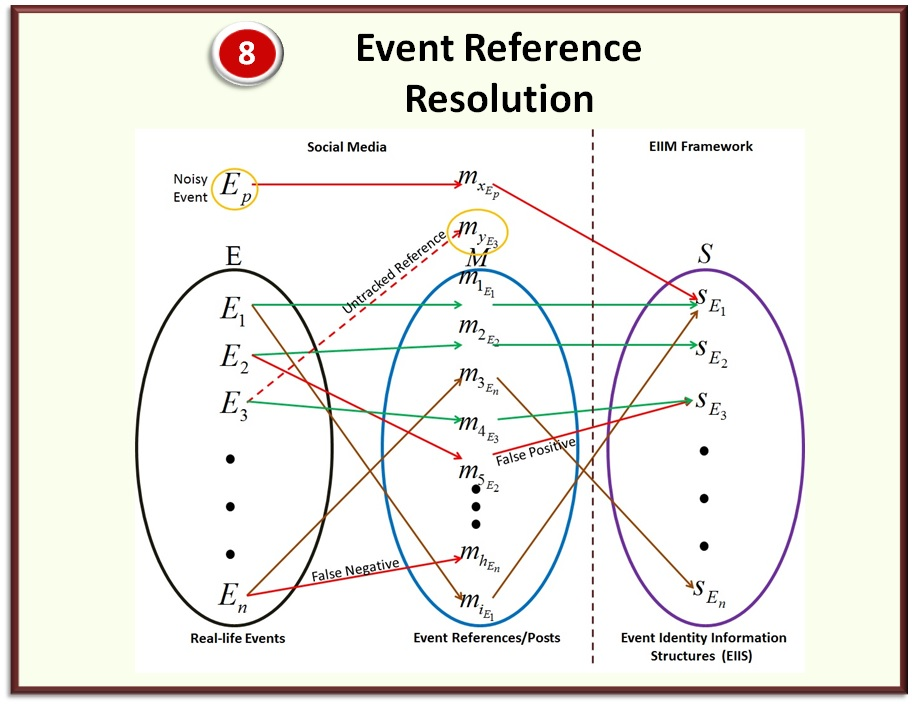
\includegraphics[width=14cm,height=11cm]{Figures/EventReferenceResolution.jpg}
\end{figure}

One of the main aims of the EIIM framework is to assign the reference of an event $E_{i}$ to its corresponding Entity Identity Information Structure ($s_{E_{i}}$). This aim is executed by this component. The main functions are as follows:

\begin{itemize}
\item The output of the previous component assigns a final ranked event-specific informativeness scores to the tweets. Using this score the component allows to choose top k tweets ranked in terms of their event-specific informative content. This enable the identification and resolution of high quality tweets providing useful information about the event $E_{i}$, solving the problems of \textit{noisy events} and \textit{noisy references} as already discussed in Chapter \ref{events}, Section \ref{problem}. The tweets after the top K are thrown away from the EIIS. This results in extremely high quality, event-specific informative tweets in the EIIS. We performed our experiment on the two events:

\begin{itemize}
\item Sydney Siege Crisis
\item Millions March NYC
\end{itemize}

Excerpts of the top 5 tweets identified for both the events are given below.

\textbf{Top Five Event-specific Informative Tweet Excerpts for Sydney Siege Event}
\begin{enumerate}
\item RT @faithcnn: Hostage taker in Sydney cafe has demanded 2 things: ISIS flag and; phone call with Australia PM Tony Abbott \#SydneySiege http://t.co/a2vgrn30Xh
\item Aussie grand mufti and; Imam Council condemn \#Sydneysiege hostage capture http://t.co/ED98YKMxqM - LIVE UPDATES http://t.c...
\item RT @PatDollard: \#SydneySiege: Hostages Held By Jihadis In Australian Cafe - WATCH LIVE VIDEO COVERAGE http://t.co/uGxmd7zLpc \#tcot \#pjnet \\ sydney-siege-scene/index.html
\item RT @FoxNews: MORE: Police confirm 3 hostages escape Sydney cafe, unknown number remain inside http://t.co/pcAt91LIdS \#Sydneysiege
\item Watch \#sydneysiege police conference live as hostages are still being held inside a central Sydney cafe http://t.co/OjulBqM7w2 \#c4news
\end{enumerate}

\item The other task that can be achieved using this component is the extraction of extremely informative features from the ranked results of the previous component and use them to form an evolutionary classifier or a feature vector for constantly tracking the event tweets w.r.t time. But the feature may get updated as the event progresses and a new set of ranked features needs to be obtained from the previous component after an interval of time that should be configurable. This, functionality of the component is currently not implemented and tested. We consider it as one of our future works.
\end{itemize}


\section{Event Analytics}
\begin{figure}[htbp]
  \caption{Event Analytics component of the EIIM life cycle.}
  \centering
    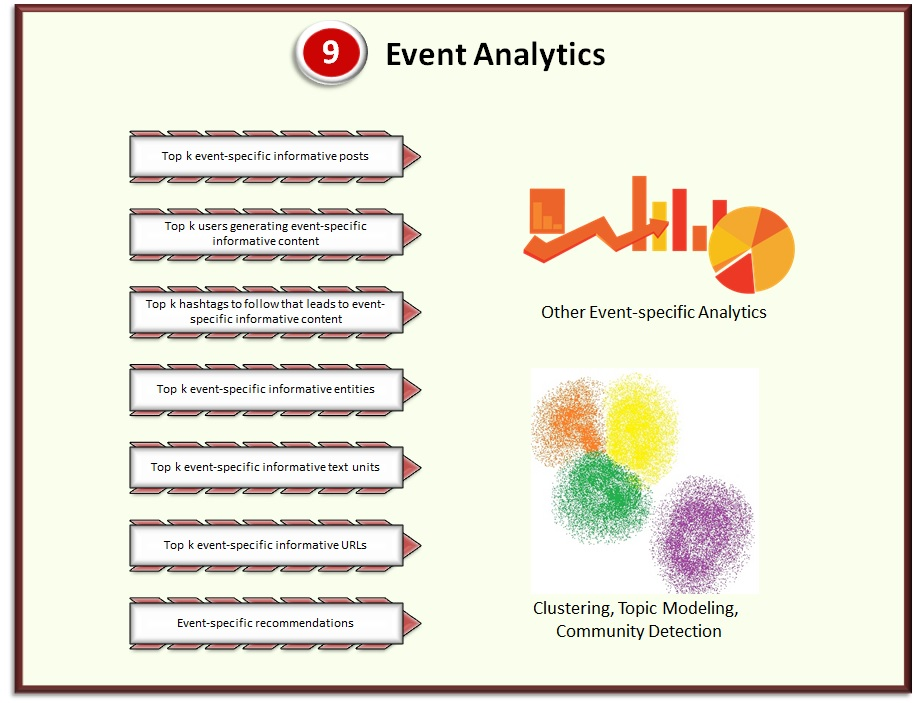
\includegraphics[width=14cm,height=11cm]{Figures/EIIMComponents/EventAnalytics.jpg}
\end{figure}

The outputs of the Event Identity Information Processing component after processing the EventIdentityInfoGraph of a particular event is used for generating different analytics related to the event for the chosen time period, by this component. Some of the immediately available analytics that help in extracting deeper insights from the event related content are shown below for our sample events.

\textbf{Top Five Event-specific Informative Hashtags for Sydney Siege Event}
\begin{enumerate}
\item \#sydneysiege 
\item \#SydneySiege
\item \#Sydneysiege
\item \#MartinPlace
\item \#9News                                                                                                                                                                                                                                                                                                                                                                                                                                                                                                                 
\end{enumerate}

\textbf{Top Five Event-specific Informative Text Units for Sydney Siege Event}
\begin{enumerate}
\item police
\item sydney
\item reporter
\item lindt
\item isis                                                                                                                                                                                                                                                                                                                                                                                                                                                                                                                
\end{enumerate}

\textbf{Top Five Event-specific Informative URLs for Sydney Siege Event}
\begin{enumerate}
\item http://www.cnn.com/2014/12/15/world/asia/australia-sydney-hostage-situation/\\index.html
\item http://www.bbc.co.uk/news/world-australia-30474089
\item http://edition.cnn.com/2014/12/15/world/asia/australia-sydney-siege-scene/\\index.html
\item http://rt.com/news/214399-sydney-hostages-islamists-updates/ 
\item http://www.newsroompost.com/138766/sydney-cafe-siege-ends-gunman-among-two-killed                                                                                                                                                                                                                                                                                                                                                                                                                                                                                                                
\end{enumerate}





\textbf{Three Randomly Selected Tweets for Top Three Event-specific Informative Users posting about Sydney Siege Event.}
\begin{enumerate}
\item \textbf{User 1}
\begin{enumerate}
\item RT @cnni: Hostage taker in Sydney cafe demands ISIS flag and call with Australian PM, Sky News reports. http://t.co/a2vgrn30Xh \#sydneysiege
\item RT @DR\_SHAHID: Hostage taker demands delivery of an \#ISIS flag and a conversation with Prime Minister Tony Abbott http://t.co/xTSDMKCPcD
\item RT @SkyNewsBreak: Update - New South Wales police commissioner confirms five hostages have escaped from the Lindt cafe in Sydney \#sydneysiege
\end{enumerate}

\item \textbf{User 2}
\begin{enumerate}
\item RT @smh: NSW Police Deputy Commissioner Catherine Burn will hold a press conference to update on the \#SydneySiege at 6.30pm.
\item RT @Y7News: Helpful travel advice for commuters heading out of \#Sydney’s CBD this evening - http://t.co/aQx2lvSosm \#sydneysiege
\item RT @hughwhitfeld: British PM David Cameron informed of \#sydneysiege ..UK Foreign Office is in touch with Aus authorities
\end{enumerate}

\item \textbf{User 3}
\begin{enumerate}
\item RT @RT\_com: \#SYDNEY: Gunman tall man in late 40s, dressed in black – eyewitness http://t.co/m51P8dUPhB \#SydneySiege http://t.co/NvJzFsGrFN
\item RT @NewsAustralia: 2GB's Ray Hadley claims hostage takers in \#SydneySiege "wants to speak to Prime Minister Abbott live on radio."
\item RT @BBCWorld: "Profoundly shocking" -Australia PM Tony Abbott delivers second \#sydneysiege statement. MORE: http://t.co/VaKt3ZpRZR
\end{enumerate}

\end{enumerate}

\textbf{Top Five Event-specific Informative Hashtags for Millions March NYC Event}
\begin{enumerate}
\item \#MillionsMarchNYC
\item \#BlackLivesMatter
\item \#ICantBreathe
\item \#ShutItDown
\item \#millionsmarchnyc                                                                                                                                                                                                                                                                                                                                                                                                                                                                                                                 
\end{enumerate}

\textbf{Top Five Event-specific Informative Text Units for Millions March NYC Event}
\begin{enumerate}
\item police
\item nyc
\item eric
\item protesters
\item nypd                                                                                                                                                                                                                                                                                                                                                                                                                                                                                                                
\end{enumerate}

\textbf{Top Five Event-specific Informative URLs for Millions March NYC Event}
\begin{enumerate}
\item http://rt.com/usa/214203-protests-police-brutality-nationwide/\\index.html
\item http://mashable.com/2014/12/13/time-lapse-new-york-protest-march/?utm\_cid=mash-com-Tw-main-link
\item http://www.cbsnews.com/news/eric-garner-ferguson-missouri-protesters-converge-on-washington/
\item http://www.huffingtonpost.com/2014/12/13/millions-march-nyc\_n\_6320348.html?ncid=tweetlnkushpmg00000051 
\item https://www.youtube.com/watch?v=Iz7hkfNmfTY\&feature=youtu.be                                                                                                                                                                                                                                                                                                                                                                                                                                                                                           
\end{enumerate}


\textbf{Three Randomly Selected Tweets for Top Three Event-specific Informative Users posting about Millions March NYC Event for a particular hour.}
\begin{enumerate}
\item \textbf{User 1}
\begin{enumerate}
\item RT @mashable: Timelapse video reveals massive size of New York City protests http://t.co/zhqHpkDLk1 \#MillionsMarchNYC http://t.co/WktxssAfDp
\item RT @DahmPublishing: RT@wendycarrillo: Real thugs wear flag pics and Eric Garner's eyes are haunting image \#MillionsMarchNYC http://t.co/7wY…
\item RT @TheRoot: RT @mfmartinez: Protesters continue gathering in Washington Square Park \#MillionsMarchNYC \#TheRootMOW http://t.co/IwkQG1KjFg
\end{enumerate}

\item \textbf{User 2}
\begin{enumerate}
\item RT @roqchams: Thousands march on NYPD headquarters to protest police terrorism http://t.co/yVyUVYkd9X http://t.co/X4QZrfOISh \#MillionsMarchNYC
\item RT @NYjusticeleague: Hundreds killed. Ten Demands. One Continued Fight.  Sign our petition at: http://t.co/KETNo6bS0V \#MillionsMarchNYC htt…
\item RT @cobismith: Union Square now with NYPD in foreground, \#MillionsMarchNYC protesters at right and; US national debt ticker on the left http:/…
\end{enumerate}

\item \textbf{User 3}
\begin{enumerate}
\item RT @mashable: Timelapse video reveals massive size of New York City protests http://t.co/zhqHpkDLk1 \#MillionsMarchNYC http://t.co/WktxssAfDp
\item RT @KeeganNYC: LOTS of NYPD waiting for protesters on the BK side of the Brooklyn Bridge \#MillionsMarchNYC \#ShutItDown \#ICantBreathe http:/…
\item RT @Zegota42: . @KeeganNYC Protesters on Brooklyn Bridge leaving Manhattan Skyline behind. \#MillionsMarchNYC \#ICantBreathe http://t.co/UPvN…
\end{enumerate}

\end{enumerate}


Some of the other event analytics that can be readily done using the \textit{EventIdentityInfoGraph}, and we would like to explore in the near future are:
\begin{itemize}
\item Topic modeling.
\item Event-specific recommendations.
\item Clustering and Cluster Analysis.
\item Community detection.
\item Trend Analysis.
\end{itemize}

The event related data stored in the database by the `Event Reference Collection' would allow to do all types of analysis that are popular in social media.

 
% Chapter 7

\chapter{Evaluations} % Main chapter title

\label{eval} % For referencing the chapter elsewhere, use \ref{Chapter1} 

\lhead{Chapter 7. \emph{Evaluations}} % This is for the header on each page - perhaps a shortened title

%\section{Conclusion}
%
%\section{Future Work}
%
%\subsection{Summarizing Event Related Content}
%
%\subsection{Identifying Insightful Opinionated Content Related to Events}
%
%\subsection{Event Topic Modeling}
%
%\subsection{Event-specific Recommendations}
%
%\subsection{Distributed Processing of EventIdentityInfoGraph}
%
%\subsection{Event Ontology for Social Media}

\section{Evaluation Baselines}

In order to evaluate the performance of \textit{EventIdentityInfoRank} we selected six different techniques that acted as our baselines. The six techniques along with their brief explanation and the reason behind their choice is discussed below.

\begin{enumerate}
\item \textbf{LexRank} - LexRank is a popular graph based algorithm commonly used in summarization of textual documents \cite{erkan2004lexrank}. It uses a stochastic graph-based method for computing the relative importance of textual units for Natural Language Processing. The task of extractive text summarization is based on the concept of identifying the most important sentences in a document or a set of documents. Importance is defined in terms of the presence of particular important words or in terms of similarity to a centroid pseudo-sentence. LexRank, computes sentence importance based on the concept of eigenvector centrality in a graph representation of sentences. In this model, a connectivity matrix based on intra-sentence cosine similarity is used as the adjacency matrix of the graph representation of sentences. We implement the LexRank algorithm using an open-source python module named sumy\footnote{\tiny https://pypi.python.org/pypi/sumy/0.1.0}, and rank the event related tweets considering them as individual sentences.

The objective of ranking natural language sentences in terms of their importance, makes it very similar to the \textit{EventIdentityInfoRank} algorithm as proposed in this dissertation for the purpose of ranking tweets instead of textual documents. \textit{EventIdentityInfoRank}, additionally ranks other units of information such as hashtags, text units, users and URLs, simultaneously, and does not takes into account the similarity of the tweets with a centroid pseudo-tweet. 

\item \textbf{TextRank} - TextRank is another popularly used technique used for summarization of textual documents \cite{Mihalcea2004}.  It is also a graph-based
ranking model for text processing, that can be successfully used in natural language
applications. The mechanism of its working is very similar to PageRank. However, instead of ranking web pages based on their linking structure, it ranks text units based on their linking structure. It can be used for identifying salient sentences as well as key words of a document. Its objective of identifying key words and important sentences is also similar to our objective of finding important tweets.

In our implementation, we modified the algorithm in order to make it suitable for our context. Apart from creating heterogeneous relationships in \textit{EventIdentityInfoGraph} we also created homogeneous relationships between the \textit{event identity information units}. Cosine similarity ($ \ge 0.10$) was used as the measure of relatedness between tweets, and the association scores of the hashtags, text units, users and URLs were based on their co-occurrence normalized between 0 and 1. The users were associated whenever they mentioned each other in the tweets, and the association score was measured by the number of mentions normalized between 0 and 1.


\item \textbf{Centroid} - Centroid is one of the techniques that was previously used in the literature for solving a part of our problem that ranks tweets. The technique is used for identifying high quality informative and useful tweets related to an event   \cite{becker2011selecting}. In order to implement it as a baseline we considered the tweets for the event in the given time period as one cluster. After preprocessing the tweets, we calculated the centroid of the cluster and ordered the tweets in the decreasing order of their similarities with the centroid.

\item \textbf{SeenRank} - SeenRank is a proprietary algorithm commercially used by Seen.co for generating event summaries and highlights from Twitter. We considered \textit{SeenRank} as the state-of-the-art technique. Although the true working of the algorithm is unknown, yet the task that the algorithm achieves is similar to the task of \textit{EventIdentityInfoRank}. In order to use this technique as one of our baselines. we also collected the tweets about the events tracked by our framework from Seen.co. The collection task was achieved using their API found at http://developer.seen.co/, and a freely available python wrapper pySeen\footnote{https://github.com/dxmahata/pySeen}, for collecting data from Seen.co. Each tweet collected from the website has a score assigned to it using SeenRank. We use this score for arranging the tweets in descending order. The ordering of the tweets were confirmed from the company's co-founder in order to be sure that greater score reflects higher ranking.



\item \textbf{RTRank} - Number of retweets is a good measure of popularity of a tweet and is also used by Twitter for ranking its search results. It is also commonly used by other paltforms for ranking tweets as already pointed out in Chapter \ref{review}. Therefore, we also considered tweets ordered in decreasing order of number of retweets as one of our baselines. We name this scheme as RTRank.

\item \textbf{Logistic Regression Model} - This technique is the logistic regression model that we implemented for initializing the informativeness score of the tweets in the `Event Information Quality' component. The generic informativeness score assigned by the logistic regression model is different from the final event-specific informativeness score assigned by \textit{EventIdentityInfoRank}. Also the logistic regression model acts as a good representative of supervised approaches. We explain this with an example.

On manually analyzing the informative tweets we tried to assess if it is good enough to train a classifier for detecting informative tweets for an event in order to identify valuable event-specific information. Although the tweets on which we trained our logistic regression model were related to events yet we came across tweets like, \textit{RT @BFDealz: http://t.co/TSJAigrVJI WHEELS SUPER TREASURE HUNT SUPERIZED HARLEY DAVIDSON FAT BOY LONG CARD 2014 \#cpac2014 \#sxsw}, which were classified as informative, even when it did not contain any event-specific information. 

This was probably because of the choice of features for the model, which were generic and not event-specific. The model did not take into account the presence of features that were popular and specific to the events, like popular hashtags, text units, etc. Popularity alone might not work as it is often mis-used by the spammers. It is also challenging to come up with a list of such event-specific features. Moreover, if one can compile such a list then it would be difficult to set thresholds on each such feature in order to qualify it as event-specific. Also, a supervised classification model does not have the ability to simultaneously rank tweets, hashtags, text units, URLs and users in terms of event-specific informativeness. After going through the existing literature we assume that the challenges discussed above would be a shortcoming of any supervised model and there is a need for an alternative feasible approach. It is also difficult to predict the event-specific informativeness in the URLs shared along with the tweets, as it might be necessary to analyze the content pointed to by the URLs. Also, not all the URLs contain text. They might be images or videos providing valuable information about an event. This motivated us to devise a novel framework that solves all the above problems.


Therefore, we considered the model as one of our baselines in order to make sure that our \textit{EventIdentityInfoRank} improves upon the initial generic informativeness score already assigned to the tweets at the start of the iteration and assigns event-specific informativeness scores on convergence. In other words the tweets having high score after the final ranking are more useful and informative than the initial ranking obtained using the logistic regression model.

\end{enumerate}


Due to unavailability of proper baseline techniques for ranking hashtags, text units, URLs and users in terms of event-specific informativeness we do not compare the results obtained for them with any other approach. However, we report their average scores and sample results. Please refer the previous chapter for the sample results.

\section{Evaluation Setup and Objectives}
We evaluated the rankings obtained using \textit{EventIdentityInfoRank} on the  datasets (refer Chapter \ref{eiim}, `Event Reference Collection' component), collected for events: ``Millions March NYC'' and ``Sydney Siege Crisis", by comparing its performance with the selected baselines. A subset of tweets for each event for a given time period (one hour) was selected. The choice of the time period was made on the basis of the interesecton of the time period of the tweets collected by us and that provided by Seen for the same event. There were 21641 tweets for Millions March NYC and 37429 tweets for Sydney Siege, respectively. We obtained the ranked tweets for all the seven approaches. For all the approaches except \textit{SeenRank} the tweets were sorted in decreasing order on the basis of the ranking scores as the primary key and time of posting as the secondary key. This was done in order to get the most informative yet recent tweets at the top of the order. For \textit{SeenRank} we sorted the tweets in terms of the scores assigned to them by Seen, as showing recent informative tweets for an event is one of the features of their platform.

We then followed a standard user evaluation approach to judge the event-specific informativeness of ranked tweets and also the hashtags, text units, URLs, and users.  A team of three independent annotators comprising of graduate students, having taken the course of Information Retrieval, were assigned the task of annotation. Necessary background of the events were given to the annotators along with suitable resources for learning more about the events. Next, we present the annotation schemes.

\begin{table}[htbp]
\centering
\caption{Avg IIC scores and total avg scores of annotations for Millions March NYC event.}
\label{avgiicMillionsMarchNyc}
\begin{tabular}{|c|c|c|}
\hline
\textbf{\begin{tabular}[c]{@{}c@{}}Millions March \\ NYC\end{tabular}} & \textbf{IIC} & \textbf{\begin{tabular}[c]{@{}c@{}}Total Avg \\ Score (1-3)\end{tabular}} \\ \hline
\textbf{\begin{tabular}[c]{@{}c@{}}Top 50 event-specific\\ informative Hashtags\end{tabular}} & 0.786 & 1.980 \\ \hline
\textbf{\begin{tabular}[c]{@{}c@{}}Top 50 event-specific\\ informative Text Units\end{tabular}} & 0.880 & 1.320 \\ \hline
\textbf{\begin{tabular}[c]{@{}c@{}}Top 50 event-specific\\ informative URLs\end{tabular}} & 0.926 & 2.560 \\ \hline
\textbf{\begin{tabular}[c]{@{}c@{}}Top 50 event-specific\\ informative Users\end{tabular}} & 0.700 & 2.386 \\ \hline
\textbf{\begin{tabular}[c]{@{}c@{}}Top 100 event-specific\\ informative Tweets\end{tabular}} & 0.760 & 2.59 \\ \hline
\end{tabular}
\end{table}

\begin{table}[htbp]
\centering
\caption{Avg IIC scores and total avg scores of annotations for Sydney Siege event.}
\label{avgiicSydneySiege}
\begin{tabular}{|c|c|c|}
\hline
\textbf{Sydney Siege} & \textbf{IIC} & \textbf{\begin{tabular}[c]{@{}c@{}}Total Avg\\ Score (1-3)\end{tabular}} \\ \hline
\textbf{\begin{tabular}[c]{@{}c@{}}Top 50 event-specific\\ informative Hashtags\end{tabular}} & 0.880 & 2.027 \\ \hline
\textbf{\begin{tabular}[c]{@{}c@{}}Top 50 event-specific\\ informative Text Units\end{tabular}} & 0.986 & 1.487 \\ \hline
\textbf{\begin{tabular}[c]{@{}c@{}}Top 50 event-specific\\ informative URLs\end{tabular}} & 0.893 & 2.413 \\ \hline
\textbf{\begin{tabular}[c]{@{}c@{}}Top 50 event-specific\\ informative Users\end{tabular}} & 0.646 & 2.353 \\ \hline
\textbf{\begin{tabular}[c]{@{}c@{}}Top 100 event-specific\\ informative Tweets\end{tabular}} & 0.83 & 2.62 \\ \hline
\end{tabular}
\end{table}

\subsection{Tweet Annotation} 
The ranked tweets were annotated on an event-specific informativeness-scale of 1 to 3 by the three independent annotators. We provide sample tweets for each of them taking the Sydney Siege event as our example. 

\begin{itemize}
\item The value of 1 was assigned to tweets that does not contain any event related information (for e.g. \textit{SteveSmith becomes Australias 45th Test captain http://t.co/nYh9DqRXxh \#sydneysiege \#MartinPlace Lindt \#MYEFO \#siege Ray Hadley Muslims ISIS}). 
\item Value of 2 was assigned to tweets that were related to the event yet they did not provide useful event-specific information (for e.g. \textit{RT @TheDavidStevens: It wasn't just the policeman grabbing that girl in his arms, it was every Australian watching on too \#sydneysiege} ). 
\item A value of 3 was assigned to tweets that not only provided useful event-specific informative content but also led the user to more detailed information following the URLs mentioned in the tweet (for e.g. \textit{RT @FoxNews: MORE: Police confirm 3 hostages escape Sydney cafe, unknown number remain inside http://t.co/pcAt91LIdS \#Sydneysiege}).  
\end{itemize}



The annotators assigned scores to top 100 tweets ranked according to each of the seven strategies. Thereafter, we computed \textit{Inter Indexer Consistency} (IIC) values \cite{rolling1981indexing} for the annotations of the two datasets. The average IIC scores obtained for the two events are are shown in Table \ref{avgiicMillionsMarchNyc} and Table \ref{avgiicSydneySiege}, respectively. The IIC values for both the events fall in the acceptable range of accuracy of annotations. A tweet might be assigned three different scores by the annotators. In that scenario we find the average of the three scores and round it off to the smallest positive integer and assign a single score to each tweet. We also report the total average scores for top 100 tweets for both the events in the tables. 

\subsection{Hashtags, Text Units and URL Annotations}
A similar annotation strategy was taken for annotating the top 50 hashtags, text units and URLs obtained using \text{EventIdentityInfoRank}. For hashtags and text units the annotators were asked to look at the tweets that consisted them. Following strategy was followed for scoring.

\begin{itemize}
\item If the tweets containing them primarily led to event-specific informative content then a score of 3 was assigned.

\item If the tweets containing them led to related but not so informative content about the event then they were assigned a score of 2.

\item Hashtags and text units that were irrelevant and did not lead to any event related content, were assigned a score of 1.
\end{itemize}

Similarly, the annotators visited the links for each URL, and based on the content they assigned them a score between 1-3. If the URLs were videos and images, then they further visited the tweet containing them in order to understand the context and scored them accordingly. Table \ref{avgiicMillionsMarchNyc} and Table \ref{avgiicSydneySiege} shows their average IIC scores and total average scores for top 50 ranks. 

\subsection{User Annotations} 
For annotating users we selected 5 random tweets for each of the top 50 users ranked according to \textit{EventIdentityInfoRank}. An user was assigned a score of 3 if more than three of his tweets out of five got a score of 3 in the event-specific informativeness scale as already explained earlier. If three of his tweets get a score of 3 then the user gets a score of 2. Otherwise, a score of 1 is assigned to the user. Table \ref{avgiicMillionsMarchNyc} and Table \ref{avgiicSydneySiege} shows average IIC scores and total average scores for top 50 users.

 
\subsection{NDCG@n and Precision@n}
After being assured about consistency and accuracy of annotations, we moved to compute the \textit{Normalized Discounted Cumulative Gain} (NDCG) \cite{jarvelin2002cumulated} and Precision \cite{baeza1999modern} values at each of the hundred recall levels. The NDCG values consider both the position and event-specific informativeness scores of the tweets. The NDCG value up-to position $p$ in the ranking is given by equation \ref{eq62}, where $DCG_{p}$ denotes the \textit{discounted cumulative gain up-to position p} and is calculated using equation \ref{eq61}, and $IDCG_{p}$ denotes the \textit{ideal discounted cumulative gain} value till position $p$ in the ranking, or in other words the maximum possible $DCG_{p}$ value till position $p$. $rel_{i}$ denotes the graded relevance of the result at position $i$. In the context of our evaluation $rel_{i}$ represents the average rounded score in the scale of (1-3) that has been assigned by the annotators to the tweet at position  $i$ in the ranked list of top 100 tweets.

\begin{equation}
\label{eq61}
DCG_{p} = \sum_{i=1}^{p}\frac{2^{rel_{i}}-1}{log(i+1)}
\end{equation}

\begin{equation}
\label{eq62}
nDCG_{p} = \frac{DCG_{p}}{IDCG_{p}} 
\end{equation}

Precision@n is measured using equation \ref{eq63}. A tweet was considered to be relevant if it has a score of either 3 or 2 and was considered irrelevant if it has a score of 1.

\begin{equation}
\label{eq63}
\frac{No.\,of\, relevant\, tweets\, at\, position\, n}{n}
\end{equation}

NDCG@n and Precision@n values were calculated for all the seven approaches for each of the datasets. Figures \ref{millionsmarchndcg} and \ref{sydneysiegendcg} shows the NDCG curves for all the seven approaches on the Millions March NYC and the Sydney Siege events, respectively, for up-to 20 recall levels. Tables \ref{sydneysiegendcgtable} and \ref{sydneysiegeprecisiontable} presents the NDCG@n values and Precision@n values for different recall levels upto 100 for the Sydney Siege Crisis event. Similarly, Tables \ref{millionsmarchndcgtable} and \ref{millionsmarchnycprecisiontable} presents the NDCG@n values and Precision@n values for different recall levels upto 100 for the Millions March Nyc event.It is quite evident from the figures and the tables that EventIdentityInfoRank approach outperforms all the baselines including the state-of-the-art approach of \textit{SeenRank} in gaining event-specific information.



\begin{figure}[htbp]
\centering
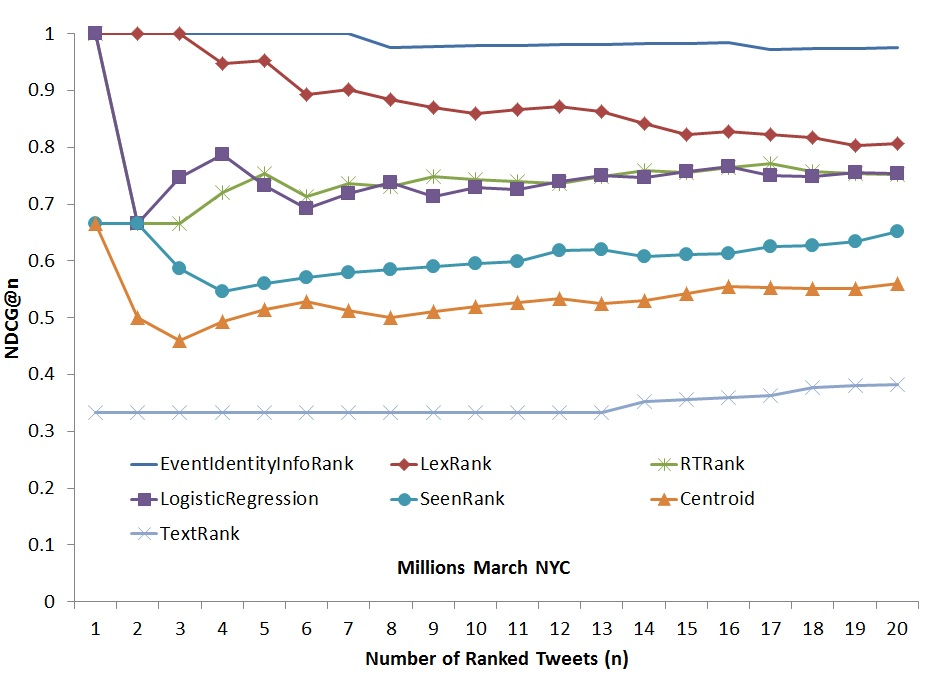
\includegraphics[height=4.5in,width=6in]{Figures/EventIdentityInfoRankPerformanceMillionsMarchNyc.jpg}
\caption{\small Performance comparison of ranking techniques using NDCG scores.}
\label{millionsmarchndcg}
\end{figure}

\begin{figure}[htbp]
\centering
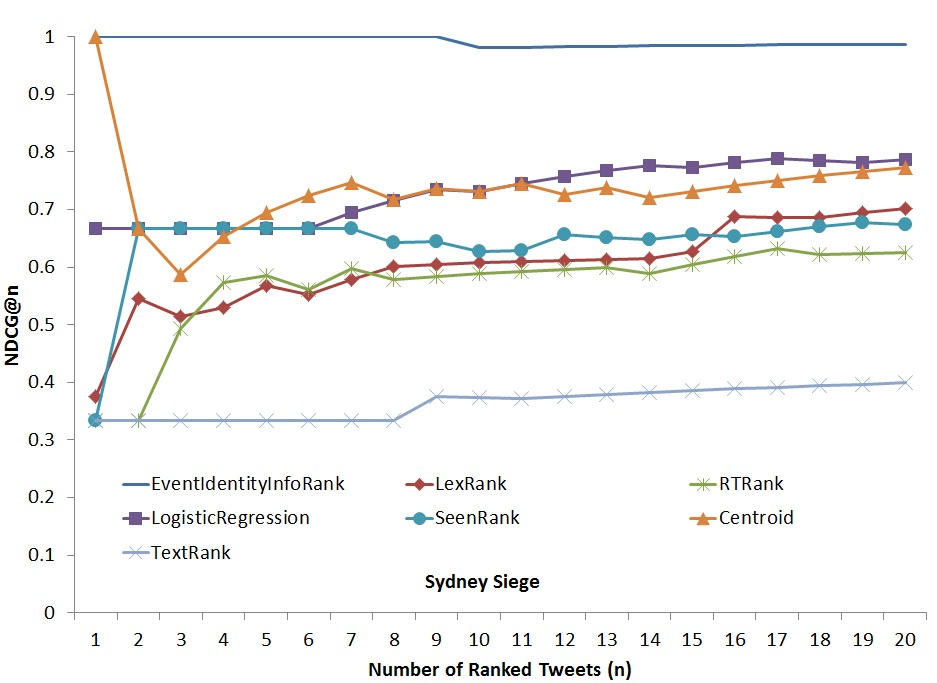
\includegraphics[height=4.5in,width=6in]{Figures/EventIdentityInfoRankPerformanceSydneySiege.jpg}
\caption{\small Performance comparison of ranking techniques using NDCG scores.}
\label{sydneysiegendcg}
\end{figure}






\begin{figure}[htbp]
\centering
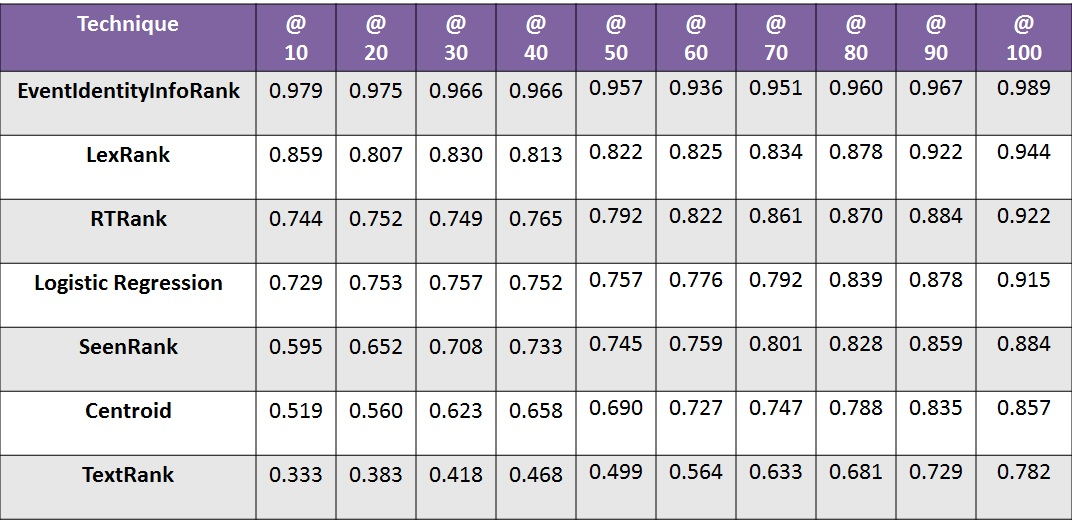
\includegraphics[height=3in,width=5.5in]{Figures/MillionsMarchNycCorrectedNDCG.jpg}
\caption{\small Performance comparison of ranking techniques using NDCG scores.}
\label{millionsmarchndcgtable}
\end{figure}

\begin{figure}[htbp]
\centering
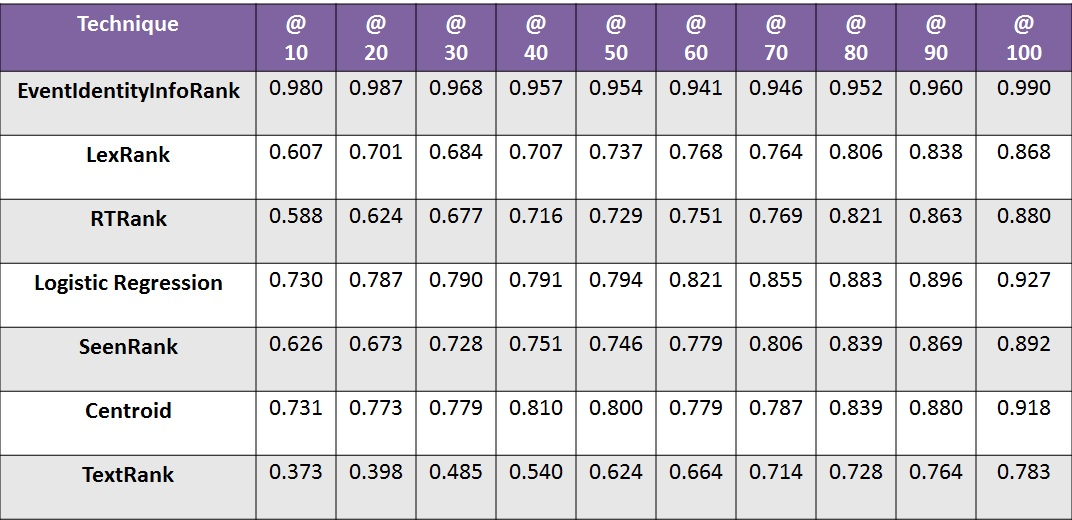
\includegraphics[height=3in,width=5.5in]{Figures/sydneysiegecorrectedndcg.jpg}
\caption{\small Performance comparison of ranking techniques using NDCG scores.}
\label{sydneysiegendcgtable}
\end{figure}

\begin{figure}[htbp]
\centering
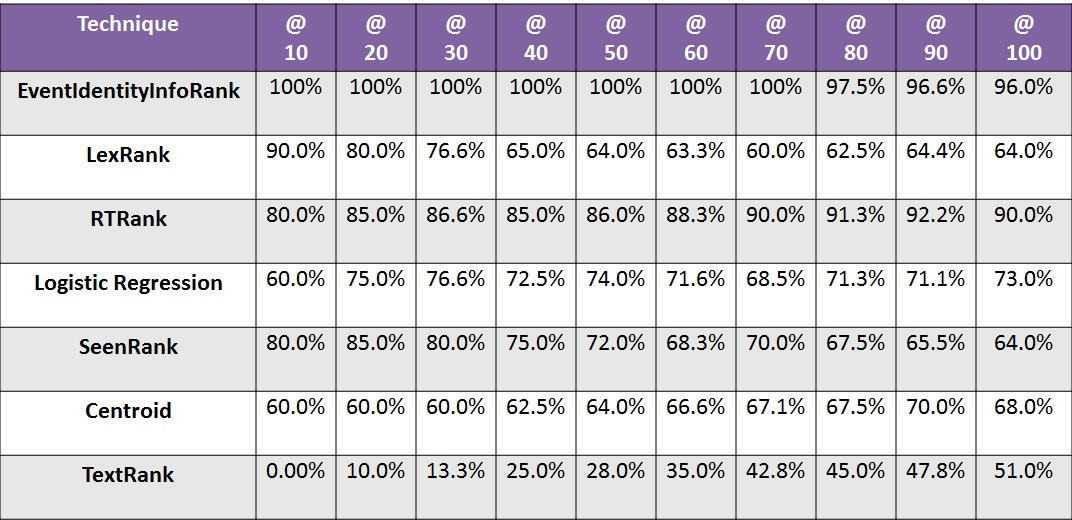
\includegraphics[height=3in,width=5.5in]{Figures/MillionsMarchNycCorrectedPrecision.jpg}
\caption{\small Performance comparison of ranking techniques using precision scores.}
\label{millionsmarchnycprecisiontable}
\end{figure}

\begin{figure}[htbp]
\centering
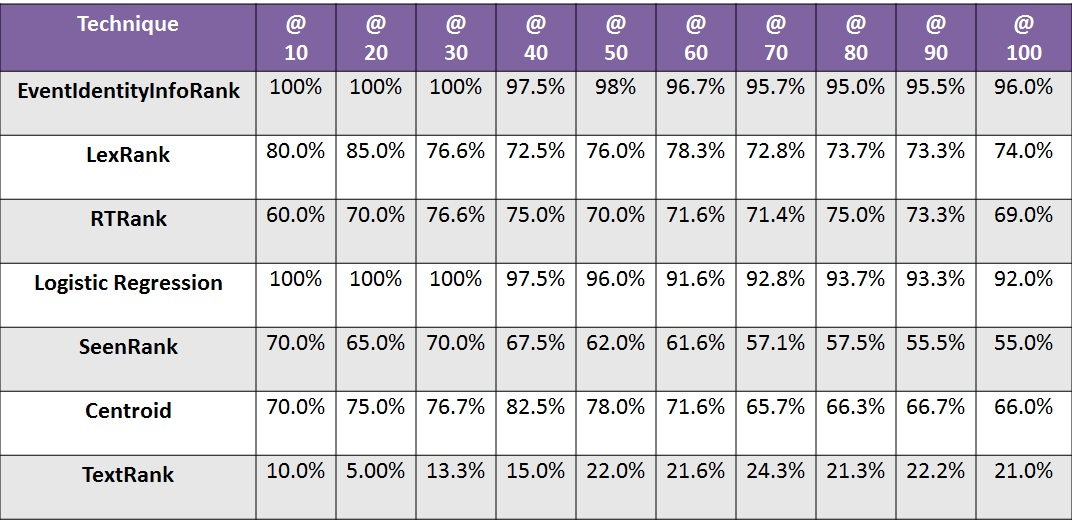
\includegraphics[height=3in,width=5.5in]{Figures/sydneysiegeprecisioncorrected.jpg}
\caption{\small Performance comparison of ranking techniques using precision scores.}
\label{sydneysiegeprecisiontable}
\end{figure}

On considering only the top 10 tweets we observed a substantial information gain of our algorithm over the state-of-the-art (\textit{SeenRank}) and the baseline that performed second best for both the events. On comparing the values of NDCG@10 for the two events we found that our algorithm performs 13.96\% (Millions March NYC) and 34.07\% (Sydney Siege) better than the second best baseline technique, in identifying event-specific informative tweets. When compared with \textit{SeenRank}, our algorithm was 64.53\% (Millions March NYC) and 56.59\% (Sydney Siege) better. 

We also reasoned about the poor performance of \textit{TextRank} in both the events. Since \textit{TextRank} allowed random walks between homogeneous nodes, the strong association of non-informative nodes with the informative ones might have lowered the final scores of the informative nodes. The strong association of non-informative nodes with informative ones can be attributed to the spamming activity as already explained earlier Chapter \ref{review}, Section \ref{veracity} This also proves that our framework is robust against spams and is very effective in identifying the most informative content related to events from the noisy stream of tweets in Twitter. 


% Chapter 8

\chapter{Potential Applications of the EIIM Framework} % Main chapter title

\label{applications} % For referencing the chapter elsewhere, use \ref{Chapter1} 

\lhead{Chapter 8. \emph{Potential Applications of the EIIM Framework}} % This is for the header on each page - perhaps a shortened title
\doublespacing
\setlength{\parindent}{1cm}
\section{Event Monitoring and Analysis}
References related to real-life events are extremely abundant in social media. Right from natural disasters such as the `Haiti Earthquake' \cite{gao2011harnessing} to international sporting events like the `Winter Olympics' \cite{walker2013russia} to socio-political \cite{singh2010mining} and socio-economical \cite{bollen2009modeling} events that shook the world such as presidential elections \cite{metzgar2009social}, `Egyptian Revolution' \cite{choudhary2012social}, and recessions were covered, analyzed, extrapolated and informed by social media. This prolific event-specific content in social media makes it a promising ground for performing event analytics. Platforms like Geofeedia\footnote{http://geofeedia.com/}, TwitterStand\footnote{http://twitterstand.umiacs.umd.edu/}, Twitris\footnote{http://twitris.knoesis.org/}, Truthy\footnote{http://truthy.indiana.edu/}, and TweetTracker\footnote{http://tweettracker.fulton.asu.edu/}  have developed techniques to provide analytics related to different local and global real-life events. 

Monitoring social media has become one of the essential activities of national security agencies for predicting potential threats and mass protests \cite{ghannam2011social}. Social media is being used for tracking terrorism activities \cite{oh2011information}, collective actions \cite{agarwal2014online}, and countering cyber-attack threats\footnote{https://www.recordedfuture.com/}. One of the main components of each of these applications is tracking references related to the events. The proposed EIIM model could be an essential component of such systems. It would help in identifying, tracking and analyzing events and its related references in an organized manner over time.



\section{Event Information Retrieval}
Retrieving informative content related to real-life events shared in social media and presenting them in an organized way to the interested users has led to web based services like Seen\footnote{http://seen.co}. It allows users to follow live updates of the events and also aids in witnessing and re-living the events at a later stage from the archives. Showing useful and interesting content to users by filtering out the pointless babbles from social media streams is an important component of such services. Additionally, such systems could get immensely benifitted by identification of event-specific informative hashtags, text units, users and URLs over time as the event proceeds. This would further enable efficient indexing of event-specific terms and hashtags that leads to high quality information, and effective processing of information. It would enhance the user experience, allowing better consumption and summarization of information related to the events, and positively impact triggering of event-specific recommendations. Thus, the proposed EIIM model in this thesis can act as the core component of information retrieval systems retrieving and organizing information related to real-life events from social media. 

\section{Opinion and Review Mining}
Every day millions of people express their opinions in social media about products and companies they like and dislike. Their communications often include thoughts about good and bad experiences with the products and services. This provides a great opportunity for companies to understand its customers and to get unbiased valuable feedback from them about their product offerings without asking them to fill out time consuming outdated surveys. The EIIM framework when used for monitoring references of products/services from social media during product launch events could be useful in mining isightful and informative opinionated content. Combined with sentiment analysis, the invention could be a powerful tool for review analysis. One of the important contributions of the system could be to identify the sources having high chances of containing insightful information and filter them out for further processing. This would make a review mining system more efficient and increase its overall quality. Mining opinions related to entities related to an event could be used in many other contexts like political campaigns, socio-political studies, market behavior analysis, e-commerce applications, etc. Steps are being taken for adding this capability to the EIIM framework as discussed in the next chapter. 

%On considering a mix of named entities and unigram opinionated words as text units in the \textit{EventIdentityInfoGraph} we obtained some preliminary encouraging results. A glimpse of the results obtained for a basketball game ''Miami Heats VS Cleveland Cavaliers", played on 25th December, 2014 is as follows:
%
%Top 10 insightful and opinionated tweets for an hour related to the game
%\begin{enumerate}
%
%\item	Good win for the Heat tonight against Cavs and Lebron. Great game for Wade and Deng. Just imagine if Bosh were healthy. \#HeatvsCavs
%
%\item	Good work Dwayne Wade. Good work Miami Heat. LeBron is embarrassed. It's all over his face. \#NBA \#heatvscavs
%
%\item	Great game on Christmas Heat Showed up and spoiled Lebron Return to MIA! \#Wade County \#HeatvsCavs \#NBAChristmas
%
%\item	Lebron leaves Miami high and dry and they cheer his return. Some even cheering cavs. Embarrassing bandwagon fan base. \#heatv…
%
%\item	I totally understand LBJ move to Cleveland and like it. But if I'm a \#Miami fan, I would boo LeBron like crazy today. \#heatvscavs \#CLEvsMIA
%
%\item	Stay classy \#Miami. Good game vs. Lebron and; Cavs. \#NBA \#MIAvsCLE \#HeatvsCavs \#Heat \#HeatNation
%
%\item Loul Deng playing both ends of the floor. He's playing good D to LBJ \#heatvscavs
%
%\item	Heat fans ; Cavs fans. Class vs no class. No burning a jersey in Miami \#heatvscavs \#HeatNation
%
%\item	WE FUCKING WON!!!!!! LETS GO HEAT \#HEATgame \#HeatNation \#HeatvsCavs Wade with 31 points 5 assist 5 rebounds! Good shit MIAMI
%
%\item	Kevin Love is overrated. Big fish, small pond in MN and injury prone. \#HeatvsCavs \#NBAXmas
%
%\end{enumerate}
%
%The above tweets point to the reactions of the viewers on the game as well as the players participating in the event.

%\section{Recommender Systems}
%The EIIM framework can be used for developing event related recommender systems. The ranked list of event identity information can be used for giving useful recommendations. For example following is a refined tweet recommendation for an event obtained from a snapshot of the \textit{EventIdentityInfoGraph} created for the event: “BlackLivesMatter”: Protest movement against the killing of Eric Garner.
%
%\textbf{Original Tweet:}
%
%\begin{itemize}
%\item \#BREAKING \#NEWS | New York City Mayor Says, \#BlackLivesMatter \\ http://t.co/qYvp8L8gDh | \#BLACK  \@HCP520
%\end{itemize}
%
%\textbf{Recommended Tweets:}
%
%\begin{itemize}
%
%\item New York: What's the plan? Where are the protests happening tonight? \#EricGarner \#BlackLivesMatter \#MichaelBrown \#ICantBreathe
%
%\item Brooklyn District Attorney to Convene Grand Jury in Case of \#AkaiGurley NBC New York http://t.co/mLlYPy39Pa \#BlackLivesMatter
%
%\item New York Today! \#ShutItDown \#economicshutdown \#BlackLivesMatter \#ICantBreathe \#EricGarner \#nojusticenoprofits http://t.co/F0TrZtx2Y5
%
%\end{itemize}
%
%Similarly an user can get other recommended users who are talking on the same topic. Hashtags and topics can also be recommended. It can further lead to clustering of similar content and discovery of communities around different topics related to the event. We wish to work on this in the future.
%
%

\section{Event Management and Marketing}
Social media is increasingly being used  by event management practitioners while organizing conferences, seminars, music festivals, fashion shows, fundraisers and various other types of planned events. Tracking and producing useful and informative content before, during and after the events in social media from the perspective of event management has proved to be extremely beneficial \footnote{http://oursocialtimes.com/using-social-media-to-make-your-event-a-dazzling-success-infographic/}. Right from promoting the events, collecting RSVPs, creating communities around topics, announcing important information, getting real-time unbiased feedbacks, to marketing right content to the users creating buzz about the events, social media plays an important role. It also helps in building long term relationships with the communities of users interested in an event and track their related activities. In such a scenario the EIIM life cycle can constantly track and persistently store salient information related to events right from its inception. The \textit{EventIdentityInfoGraph} can aid in identifying event-specific informative content and users producing them, which could further lead to effective targeting of user communities, generating event summaries, mining opinions, broadcasting interesting information, among other things related to an event.

%\section{Journalism}
%In addition to the main contributions described above, techniques presented in
%this dissertation also have some broader impacts to various other areas. Below, we
%highlight some of those impacts.
%Event Analytics on Social Media and Applications in Journalism
%Technology is rapidly shifting the ways in which information about news and events is
%13
%gathered, processed, and disseminated. Computational Journalism is the application
%of computing to the activities of journalism including information gathering, organization
%and sensemaking, communication and presentation, and dissemination and public
%response to news information, all while upholding the core values of journalism such
%as accuracy and verifiability (Diakopoulos et al., 2010; Cohen et al., 2011b; Anderson,
%2013). In recent years, some of the core areas of computing such as databases, information
%retrieval, and information visualization, are already playing important roles
%in driving many changes as news organizations re-adjust to the digital era (Cohen
%et al., 2011a; Diakopoulos et al., 2012; Flaounas et al., 2013). While Computational
%Journalism is unlikely to replace real journalists, it does enable and augment human
%journalists through computing. Therefore, we believe that the transfer and use of
%computing technology in news and journalism can be accelerated, and our work presented
%here can have a direct impact regarding computational journalism, especially
%on information gathering, organization and sensemaking.
%As we mentioned earlier, the first step in Journalism is to gather relevant information
%about news and events. Thus far, this has been done mainly based on tips
%(for breaking events) and/or journalistic investigation. While such ways still work
%quite well, social networking systems (e.g. Facebook), social awareness streams (e.g.
%Twitter), location-based social networks (e.g., Foursquare) have explicitly connected
%the “what”, the “who”, the “where”, and the “when” of reporting. Besides, with the
%ubiquity and immediacy of social media, news events often are reported on Twitter or
%Facebook ahead of traditional news media. In addition, social media has also become
%one of the few sources of local news – and life-saving information – where traditional
%media is sometimes censored by governments or even criminal organizations. These
%advantages make social media an ideal information source for journalists to gather
%more information to learn new stories and/or augment their stories.
%


\section{Social Media Data Integration}
Organizations have increasingly started integrating the data available in social media with the enterprise data\footnote{http://www.altimetergroup.com/research/reports/social-data-intelligence}. Social media data is most powerful when it is combined with daily transactional data and the master data to give a comprehensive view of customers, products and business conditions. Customers often openly talk about the products in social media and build communities around hashtags \cite{tsur2012s} related to different topics. The EIIM framework could go a long way in collecting right information about the entities of concern maintained in the enterprise databases and integrate the collected information with the already existing ones. The entity resolution aspect would further help in managing the data quality issues related to data integration. In such conditions the EIIM model proposed could be used for integrating entity information from two distinct domains of enterprise system and social media in order to gain strategic intelligence related to business of an organization. This would further help an organization in marketing, corporate communications, public relations, customer support, product development, advertising, market research, product recommendations and gaining competitive intelligence.
 
% Chapter 9

\chapter{Conclusion and Future Work} % Main chapter title

\label{Conclusion} % For referencing the chapter elsewhere, use \ref{Chapter1} 

\lhead{Chapter 9. \emph{Conclusion and Future Work}} % This is for the header on each page - perhaps a shortened title
\doublespacing
\setlength{\parindent}{1cm}
\section{Conclusion}
This dissertation introduced the idea of `Event Identity Information Management' (EIIM) from textual content in social media and discussed how it could be used for tracking unstructured references related to real-life events having impressions in social media. It also introduced the Event Identity Information Management life cycle and explained its various components. It pointed to the novel contributions in each of the component and showed the effectiveness and performance of the devised techniques against the state-of-the-art baselines. 

The characteristics of informative and non-informative content produced in 3.8 million (approx) tweets during three real-life events in Twitter were studied. Cues were obtained from the analysis for identifying informative content. It was also observed that the supervised models used for assigning informativeness scores to tweets are generic and are not always well suited for identifying event-specific informative tweets. Moreover, they don't have the ability to simultaneously identify event-specific informative hashtags, text units, URLs and users. This created an intriguing scenario and led to the need of a model that identifies and ranks event-specific informative content from Twitter.

Using the cues from the analysis it was found that hashtags used for annotating tweets, text units used for expressing the tweet content, URLs shared for providing additional information and the users posting them during an event are the main units of information that could be leveraged for measuring event-specific informativeness.  Mutually reinforcing relationships were identified between the tweets, hashtags, text units, URLs and users posting them during an event, and their associations were represented in a graph structure that forms the underlying framework for the proposed ranking algorithm. This graph is named as \textit{EventIdentityInfoGraph}. The semantics of the relationships between the vertices of the graph were defined and quantified. Initial event-specific scores were assigned to the vertices. An algorithm - \textit{EventIdentityInfoRank}, was proposed for ranking the vertices. The algorithm makes use of the mutually reinforcing chains formed between the vertices of \textit{EventIdentityInfoGraph} for propagating the event-specific scores of a vertex to its neighboring vertices. The accumulated score of the vertices after the convergence of the algorithm is used for simultaneously ranking streams of tweets, hashtags, text units, URLs and users producing them during two real-life events in terms of their event-specific informativeness. Promising results were obtained using the proposed EIIM framework. The results were evaluated by comparing the performance of our approach with six other approaches including the state-of-the-art \textit{SeenRank} algorithm used by Seen for ranking tweets displayed in their website. The approach proposed in this dissertation outperformed all the baselines by large margins for NDCG@n and Precision@n scores proving it to be the most effective and robust algorithm for identifying event-specific informative content from noisy stream of tweets in Twitter.

The problem of discovering event-specific informative content in Twitter was solved by proposing a robust and scalable `Event Identity Information Management' framework that goes through a cycle of data processing pipeline, known as the EIIM Life Cycle.  Since the features used for the proposed techniques are commonly found in most of the social media platforms, it is assumed that the EIIM Life Cycle has the potential to produce effective results in other social media channels as well. The dissertation also pointed the ability of the framework to scale in a distributed processing environment. Some of the works that can be considered as future works of this dissertation are discussed next. 


\section{Future Work}

\subsection{Summarizing Event Related Content}
Given the huge amount of content produced in social media related to real-life events, summarization of the content can be very useful in such a scenario. It can help the users to overcome the problem of information overload. One of the most important characteristics of the summarization techniques is to identify the most salient units of information from the textual posts. The \textit{EventIdentityInfoGraph} and the \textit{EventIdentityInfoRank} algorithm as proposed and implemented in this dissertation can be tuned for such a purpose. One of the steps that needs to be taken is to find how the salient event identity information units obtained as an output of \textit{EventIdentityInfoRank} can be used for constructing event summaries from short textual social media messages. We have started looking into this problem and look forward to solve it using the framework as proposed in this dissertation. One of the main advantages and novelty in solving this problem using the EIIM framework would be the capability of generating event summaries as the event evolves. 

\subsection{Identifying Insightful Opinionated Content Related to Events}
Users often share insightful opinionated content about different topics, people, organizations, in social media. Such content is also generated in the context of an event. For example, in a sporting event the fans may post a lot of opinionated content about the players. Not all of them will be insightful. Similarly, in a product launch event, the prospective customers, or the reviewers may post very insightful and opinionated reviews about the new product. This type of content is extremely useful for the prospective customers, targeted marketing and for automated systems in order to identify the positive and negative aspects of the product that is creating buzz in social media. Identification of such insightful opinionated tweets can lead to the discovery of very useful and strategic information. On considering a mix of named entities and unigram opinionated words as text units in the \textit{EventIdentityInfoGraph} we obtained some preliminary encouraging results. A glimpse of the results obtained for a basketball game ''Miami Heats VS Cleveland Cavaliers", played on 25th December, 2014 is as follows:

Top 10 insightful and opinionated tweets for an hour related to the game
\begin{enumerate}

\item	Good win for the Heat tonight against Cavs and Lebron. Great game for Wade and Deng. Just imagine if Bosh were healthy. \#HeatvsCavs

\item	Good work Dwayne Wade. Good work Miami Heat. LeBron is embarrassed. It's all over his face. \#NBA \#heatvscavs

\item	Great game on Christmas Heat Showed up and spoiled Lebron Return to MIA! \#Wade County \#HeatvsCavs \#NBAChristmas

\item	Lebron leaves Miami high and dry and they cheer his return. Some even cheering cavs. Embarrassing bandwagon fan base. \#heatv…

\item	I totally understand LBJ move to Cleveland and like it. But if I'm a \#Miami fan, I would boo LeBron like crazy today. \#heatvscavs \#CLEvsMIA

\item	Stay classy \#Miami. Good game vs. Lebron and; Cavs. \#NBA \#MIAvsCLE \#HeatvsCavs \#Heat \#HeatNation

\item Loul Deng playing both ends of the floor. He's playing good D to LBJ \#heatvscavs

\item	Heat fans ; Cavs fans. Class vs no class. No burning a jersey in Miami \#heatvscavs \#HeatNation

\item	WE FUCKING WON!!!!!! LETS GO HEAT \#HEATgame \#HeatNation \#HeatvsCavs Wade with 31 points 5 assist 5 rebounds! Good shit MIAMI

\item	Kevin Love is overrated. Big fish, small pond in MN and injury prone. \#HeatvsCavs \#NBAXmas

\end{enumerate}

The above tweets point to the reactions of the viewers for the game as well as the players participating in the event. We plan to work on this and take steps to tune the EIIM framework in order to make it better than the state-of-the-art techniques, for identifying insightful opinionated content from social media. This useful content once identified and ranked can also be used for generating opinion summaries. 







\subsection{Event-specific Recommendations}
The graph based data structure used for storing the EIIS can be used for generating event related informative recommendations in near real-time. The graph structure aids in exploring relationships between tweets, text units, hashtags, users and URLs. Moreover, the `Event Identity Information Process' component processes the EIIS and assigns event-specific informativeness scores to its vertices. These scores combined with the relationships between the vertices can be leveraged for recommending users to other users who are producing event-specific informative content. Similarly, event-specific informative tweets, URLs and hashtags can be recommended. A naive approach has been implemented. For example following is a refined tweet recommendation for an event obtained from a snapshot of the \textit{EventIdentityInfoGraph} created for the event: “BlackLivesMatter”: Protest movement against the killing of Eric Garner.

\textbf{Original Tweet:}

\begin{itemize}
\item \#BREAKING \#NEWS | New York City Mayor Says, \#BlackLivesMatter \\ http://t.co/qYvp8L8gDh | \#BLACK  \@HCP520
\end{itemize}

\textbf{Recommended Tweets:}

\begin{itemize}

\item New York: What's the plan? Where are the protests happening tonight? \#EricGarner \#BlackLivesMatter \#MichaelBrown \#ICantBreathe

\item Brooklyn District Attorney to Convene Grand Jury in Case of \#AkaiGurley NBC New York http://t.co/mLlYPy39Pa \#BlackLivesMatter

\item New York Today! \#ShutItDown \#economicshutdown \#BlackLivesMatter \#ICantBreathe \#EricGarner \#nojusticenoprofits http://t.co/F0TrZtx2Y5

\end{itemize}

Similarly an user can get other recommended users who are talking on the same topic. Hashtags and topics can also be recommended. It can further lead to clustering of similar content and discovery of communities around different topics related to the event.


\subsection{Distributed Processing of EventIdentityInfoGraph}
The \textit{EventIdentityInfoRank} algorithm processes the nodes and edges of the \textit{EventIdentityInfoGraph} iteratively to come up with a simultaneous ranking of its heterogeneous vertices. The processing of the heterogeneous nodes can be distributed and then an aggregate score can be assigned to each vertex after an individual iteration. This is perfectly suitable for implementing the algorithm in a mapreduce paradigm. Similar steps are taken by the PageRank algorithm for ranking billions of web pages at scale. We plan to use the Giraph\footnote{http://giraph.apache.org/} distributed graph processing library on top of HDFS or use Apache Spark for implementing the process of ranking the vertices of \textit{EventIdentityInfoGraph}.

\subsection{Event Ontology for Social Media}
Another research direction than can be explored in the future is to develop  an ontology for representing the extracted event identity information units. This will enable a systematic categorization of the event identity information units into different concepts that can aid in formal reasoning. Reasoning on the relationships and characteristics of individual event identity information units can lead to extraction of deeper insights. For example, questions like ``who are the people involved?", ``what are the places mentioned in the event related content?", ``how are the different people and places related to one another?", and so on. Attempts have already been made on formulating ontological representation of the multimedia content produced during events by Troncy et al. \cite{troncy2010linking}, as well as, representing social media communities \cite{breslinsemantically}. Ontologies for integrating information from different types of documents have also been proposed \cite{doerr2006towards}, that can be used for representing the social media references and the relationships between the content extracted from them. Another ontology, which is of great interest to us is the Basic Formal Ontology (BFO) \cite{smith2002basic}. This is because of the fact that BFO is an upper level ontology and has constructs for all types of entities including events. It will give the freedom of exploring the way events can be defined in social media and the representation of its related textual content. Also, BFO considers events as separate from the other types of named entities like, person or a place. This enables reasoning about the relationships between several events with a person, and vice versa. At the same time relationships between the events can be explored. 
%% Chapter 7

\chapter{Literature Review} % Main chapter title

\label{review} % For referencing the chapter elsewhere, use \ref{Chapter1} 

\lhead{Chapter 7. \emph{Literature Review}} % This is for the header on each page - perhaps a shortened title

\section{Event Identification in News Text}

\section{Event Identification in Social Media}

\section{Information Quality in Social Media}

\section{Ranking and Summarization of Short Textual Social Media Posts}

\section{Reference Tracking and Entity Resolution}
 

%----------------------------------------------------------------------------------------
%	THESIS CONTENT - APPENDICES
%----------------------------------------------------------------------------------------

\addtocontents{toc}{\vspace{2em}} % Add a gap in the Contents, for aesthetics

\appendix % Cue to tell LaTeX that the following 'chapters' are Appendices

% Include the appendices of the thesis as separate files from the Appendices folder
% Uncomment the lines as you write the Appendices

% Appendix A

\chapter{Appendix Title Here} % Main appendix title

\label{AppendixA} % For referencing this appendix elsewhere, use \ref{AppendixA}

\lhead{Appendix A. \emph{Appendix Title Here}} % This is for the header on each page - perhaps a shortened title

Write your Appendix content here.
%\input{Appendices/AppendixB}
%\input{Appendices/AppendixC}

\addtocontents{toc}{\vspace{2em}} % Add a gap in the Contents, for aesthetics

\backmatter

%----------------------------------------------------------------------------------------
%	BIBLIOGRAPHY
%----------------------------------------------------------------------------------------

\label{Bibliography}

\lhead{\emph{Bibliography}} % Change the page header to say "Bibliography"

\bibliographystyle{unsrtnat} % Use the "unsrtnat" BibTeX style for formatting the Bibliography

\bibliography{Bibliography} % The references (bibliography) information are stored in the file named "Bibliography.bib"

\end{document}  